\documentclass[11pt]{article}

% ---------- packages ----------
\usepackage[margin=1in]{geometry}
\usepackage{graphicx}
\usepackage{booktabs}
\usepackage{amsmath,amssymb}
\usepackage{siunitx}
\usepackage[numbers,sort&compress]{natbib}
\usepackage{xcolor}
\usepackage[hidelinks]{hyperref}
\usepackage{caption}
\usepackage{textcomp}
\usepackage{microtype}
\usepackage{array}
\usepackage{setspace}
\usepackage{float}
\usepackage{pifont}
\onehalfspacing

\captionsetup{font=small,labelfont=bf}
\graphicspath{{figures/}}

\newcommand{\edrunit}{\si{\metre\tothe{2/3}\per\second}}
\newcommand{\todo}[1]{\textit{\textcolor{red}{[PENDING --- #1]}}}
\newcommand{\circnum}[1]{\ding{\the\numexpr181+#1\relax}}

\title{\bfseries A Physics-Informed Convolutional Neural Network for
Predicting Clear-Air Turbulence Intensity (EDR) from ERA5 Reanalysis
and Satellite Observations}

\author{Ishaan Puri}
\date{\today}

\begin{document}
\maketitle

% =====================================================================
\begin{abstract}
Clear-air turbulence (CAT) is a growing and notoriously hard-to-predict
aviation hazard: it occurs without visible cloud cues, injures hundreds
of passengers and crew annually, and is projected to intensify as the
jet stream strengthens under climate change. Operational nowcasting
relies on systems such as NOAA's Graphical Turbulence Guidance (GTG),
which combine many physical turbulence diagnostics through a
\emph{fixed weighted sum} calibrated against categorical pilot reports;
most machine-learning alternatives, conversely, discard physics
entirely. We present a \emph{physics-informed} convolutional neural
network (CNN) that bridges the two. From a purpose-built catalogue of
150 CAT events (2005--2024) we gather ERA5 reanalysis, GOES satellite
brightness temperature, and in-situ ACARS eddy-dissipation-rate (EDR)
measurements; we compute twelve operational CAT diagnostics
(Richardson number, vertical wind shear, Ellrod indices,
frontogenesis, etc.) on three jet-stream pressure levels; and we train
an encoder--decoder CNN that emits a spatial EDR field, soft-aggregated
to the scalar EDR the labels provide. The loss embeds physical
constraints (non-negativity, shear--stratification gating, diagnostic
consistency, spatial coherence, climatological bounds). We benchmark
against a GTG-style physics surrogate and a gradient-boosted (XGBoost)
baseline, and use an ablatable satellite stream to test whether
cloud-top data adds skill over reanalysis alone. Six exploratory
analyses---seasonal/diurnal decomposition, EMD and ensemble EMD,
climate-teleconnection surrogate testing, regional ADS-B heatmaps,
satellite--EDR cross-correlation, and PCA---inform the design. Under
leakage-safe, event-grouped out-of-fold cross-validation the
physics-informed CNN attains Pearson $r=0.878$ (RMSE $0.153$~\edrunit,
AUPRC $0.867$ at the moderate threshold) and beats the XGBoost baseline on
every metric ($r=0.705$, RMSE $0.179$), evidence that the spatial
structure of the diagnostic fields carries real, learnable skill beyond
pooled summary statistics. Whether a satellite stream adds further skill
over reanalysis alone, and how the model compares to a GTG-style physics
surrogate, are the remaining open questions.
\end{abstract}

% =====================================================================
\section{Introduction}
\label{sec:intro}

\subsection{Why CAT matters}
Clear-air turbulence is turbulence in the absence of convective clouds,
typically in the strongly sheared flow near upper-tropospheric jet
streams. Because it gives no visual or conventional radar warning, it
is a leading cause of in-flight injuries. The May 2024 Singapore
Airlines SQ321 event---a sudden severe encounter that caused a fatality
and dozens of injuries---is a vivid reminder of the hazard. Living in
Singapore, this incident inspired the creation of this project. Beyond
the immediate safety cost, several studies project that CAT frequency
and intensity over busy mid-latitude corridors will rise through the
century as lower-stratospheric warming sharpens the meridional
temperature gradient and strengthens vertical wind shear
\citep{williams2017,storer2019}.

\subsection{The prediction problem}
We target the \emph{eddy dissipation rate} (EDR), the ICAO-standard,
aircraft-independent turbulence metric (units \edrunit). EDR is the
rate at which turbulent kinetic energy cascades to ever-smaller eddies
before dissipating as heat; it is estimated operationally from
quick-access-recorder (QAR) accelerations and winds
\citep{sharman2014,kim2021}. EDR is heavy-tailed and approximately
log-normal, so the rare, safety-critical severe tail is easily swamped
in a linear loss. The clear-air setting compounds the difficulty: there
is no cloud signature for an imager to key on, so prediction must come
from the \emph{dynamical state of the atmosphere}. Figure~\ref{fig:overview}
sketches the end-to-end system this paper builds.

\begin{figure}[H]
  \centering
  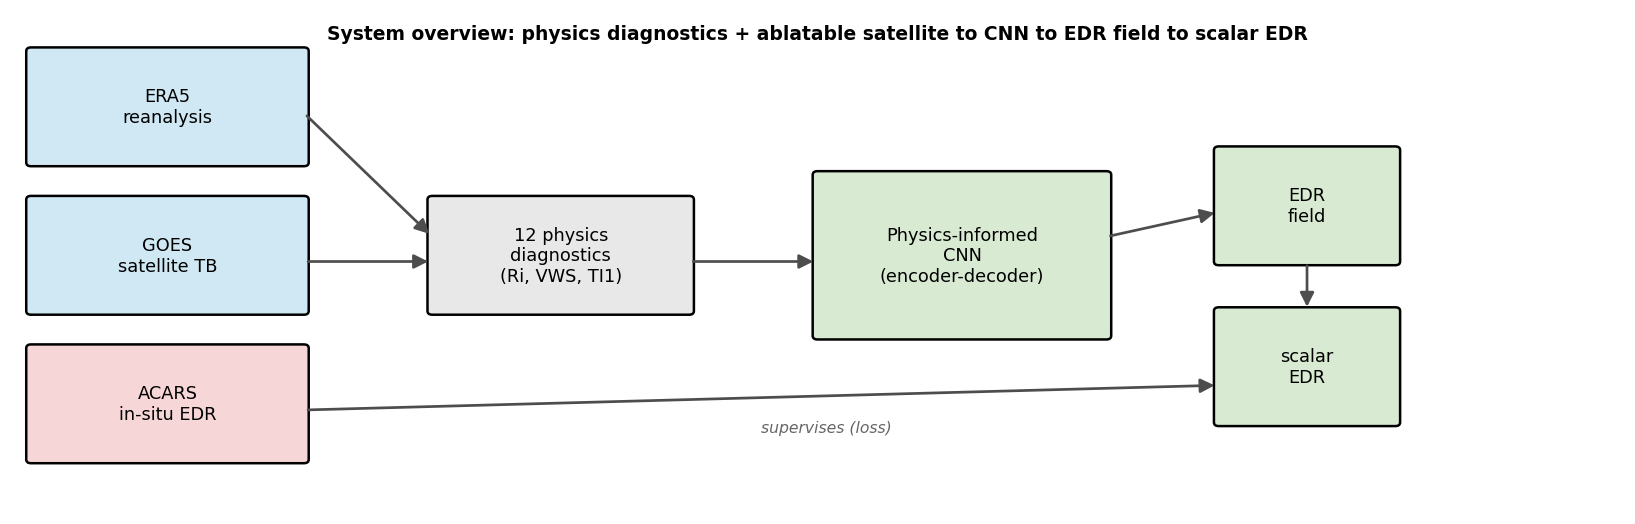
\includegraphics[width=0.80\linewidth]{pipeline_overview.png}
  \caption{System overview. ERA5 reanalysis and (optional) GOES
  satellite brightness temperature are turned into physics diagnostics,
  fed to a physics-informed encoder--decoder CNN that emits an EDR field,
  which is soft-aggregated to a scalar EDR. In-situ ACARS EDR supervises
  the scalar through the loss.}
  \label{fig:overview}
\end{figure}

\subsection{What is missing}
The dominant operational tool, NOAA GTG/GTCC, is \emph{not} a learning
system: it computes $\sim$10 upper-level and $\sim$9 mid-level turbulence
diagnostics per grid point and forms a fixed weighted sum,
$\mathrm{EDR}=\sum_i w_i e_i$, with weights tuned against categorical
PIREPs \citep{sharman2006gtg}. It ignores terrain and does not ingest
satellite cloud-top information, which carries visual precursors of
turbulence (transverse bands, billows, comma clouds). Pure-ML
approaches, in turn, often abandon the hard-won physics of CAT
diagnostics altogether.

\subsection{Contributions and research questions}
We build a physics-informed CNN that keeps the GTG diagnostic
``vocabulary'' but learns a \emph{non-linear, spatial} combination of
it, trained directly on continuous in-situ EDR rather than categorical
reports. Our questions are:
\begin{itemize}
  \item \textbf{RQ1.} Does a physics-informed CNN over reanalysis
  diagnostics predict in-situ EDR with skill beyond (a) a GTG-style
  physics surrogate and (b) a pure-ML XGBoost baseline?
  \item \textbf{RQ2.} Does satellite cloud-top brightness temperature
  add skill over reanalysis alone? We answer this structurally with an
  ablatable satellite stream.
\end{itemize}

% =====================================================================
\section{Background and Related Work}
\label{sec:background}

\subsection{CAT physics and mechanisms}
The leading CAT mechanism is Kelvin--Helmholtz (KH) instability in
stratified shear flow. Where vertical wind shear is strong enough and
static stability weak enough---quantified by a low Richardson
number---small wave-like perturbations extract energy from the mean
flow, grow, and break down into turbulence
(Fig.~\ref{fig:khmech}) \citep{williamsjoshi}. CAT is fundamentally a
\emph{mesoscale} phenomenon: the relevant structures span
$\sim$10--100\,km and observed CAT patches are typically less than
$\sim$20\,miles across, smaller than the synoptic patterns often used to
forecast them. Secondary sources include orographic lee waves
(terrain-forced gravity waves) and, near deep convection, convectively
induced turbulence (CIT).

\begin{figure}[H]
  \centering
  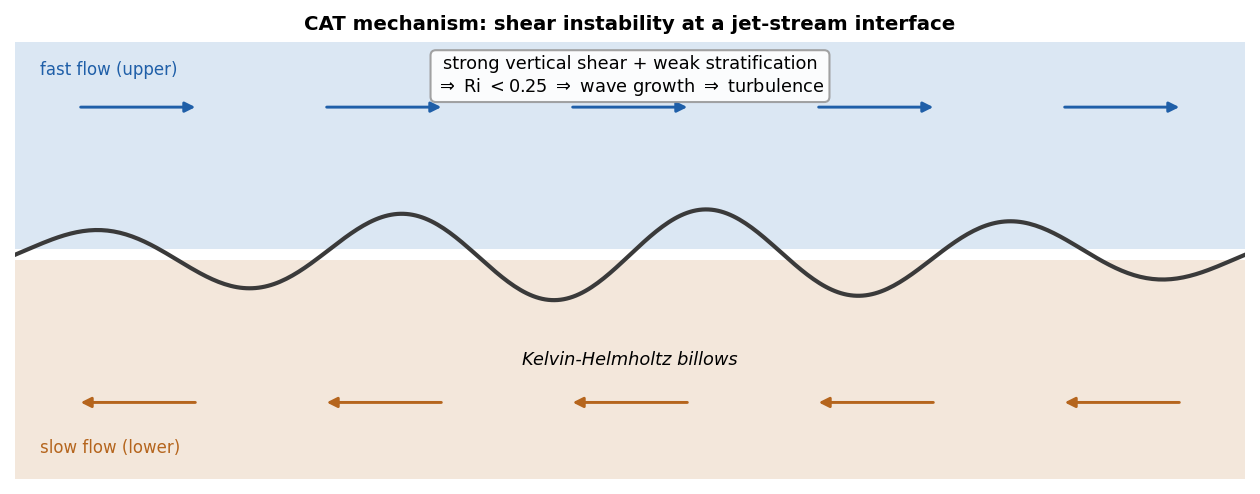
\includegraphics[width=0.80\linewidth]{kh_mechanism.png}
  \caption{Clear-air turbulence mechanism. At a jet-stream interface,
  strong vertical wind shear over weak stratification drives the
  Richardson number below the critical value ($\approx$0.25); wave-like
  perturbations grow into Kelvin--Helmholtz billows that break into
  turbulence.}
  \label{fig:khmech}
\end{figure}

\subsection{EDR as the turbulence metric}
EDR has replaced aircraft-specific load metrics as the WMO/ICAO
turbulence standard because it is intrinsic to the atmosphere rather
than to a particular airframe \citep{sharman2014}. It can be derived
from vertical acceleration or from wind-based methods on QAR data
\citep{kim2021}, and is commonly mapped through a log-normal transform
\citep{sharman2017}. We adopt the standard severity bands used
throughout: light $\geq 0.10$, moderate $\geq 0.20$, severe $\geq
0.40$~\edrunit.

\subsection{Operational nowcasting: NOAA GTG/GTCC}
GTG ingests hourly RUC/RAP model output and computes a battery of
diagnostics at each grid point, combining them as a weighted sum whose
weights are optimised against PIREPs \citep{sharman2006gtg}. Our physics
surrogate (\S\ref{sec:eval}) deliberately mirrors this design but
improves on it in three ways drawn from the literature: it optimises an
AUC objective rather than $\psi$, it regresses continuous in-situ EDR
instead of categorical PIREPs, and it uses a log-normal
diagnostic-to-EDR mapping \citep{sharman2017}.

\subsection{Machine learning for turbulence}
Prior ML pipelines typically preprocess flight data, window it, and run
parallel regression (EDR) and classification (severity) heads
\citep{icas2020}. Recurrent models (LSTMs), reduced-order/Koopman
methods, and counterfactual analyses have all been proposed; we
considered these but found a spatially-aware CNN better matched to the
mesoscale structure of CAT and to our gridded reanalysis inputs.

\subsection{Satellite signatures of turbulence}
Operational forecasters use IR/visible cloud morphology---transverse
bands, billows, comma clouds, delta cirrus, cyclonic curvature, lee
slopes---as turbulence precursors. This motivates a satellite stream,
while recognising (\S\ref{sec:eda-sat}) that pure clear-air jet CAT has
no cloud signature at all.

% =====================================================================
\section{Data}
\label{sec:data}
All data sources are open-access and gathered programmatically. A cloud
virtual machine (2 vCPU, 8\,GB) accessed over SSH handled the heavier
acquisition jobs.

\subsection{Acquisition pipeline}
The pipeline runs in five stages:
\begin{enumerate}
  \item \textbf{Event discovery.} Scan 20 years of MADIS/ACARS reports
  at 3-hourly cadence (00,03,\dots,21\,UTC), filter to FL180+, and
  cluster reports spatially (200\,km) and temporally (6\,h) with a
  6-hour early-break. Clusters are stratified into severity bins,
  expanding an initial hand-picked set of 10 events to 150.
  \item \textbf{Per-event ACARS.} Download the full $\pm$window of ACARS
  reports (turbulent and smooth) per event.
  \item \textbf{Per-event ERA5.} Pull the reanalysis fields below from
  the analysis-ready ARCO-ERA5 archive.
  \item \textbf{Per-event satellite.} Pull GOES IR
  brightness-temperature statistics.
  \item \textbf{Context.} OpenSky ADS-B state vectors for the regional
  analysis.
\end{enumerate}

The resulting catalogue and its severity distribution are summarised in
Fig.~\ref{fig:dataset}.

\begin{figure}[H]
  \centering
  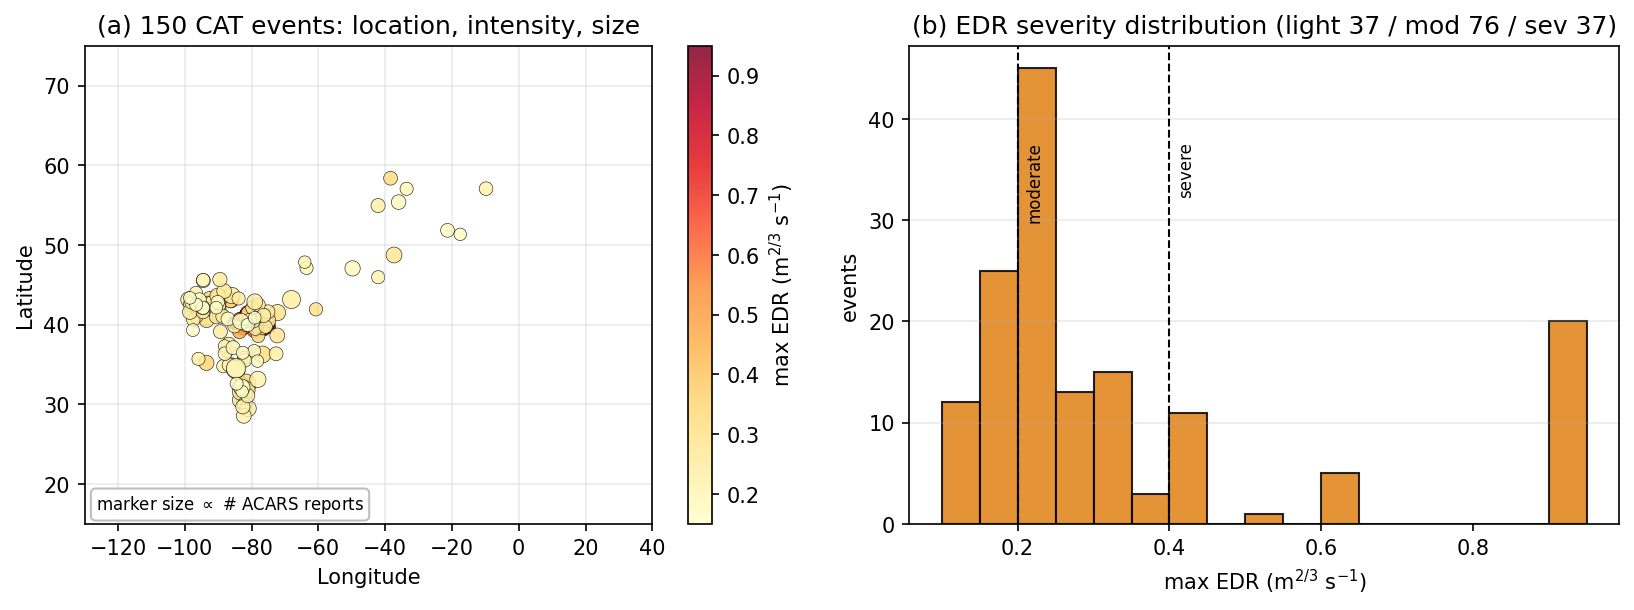
\includegraphics[width=0.85\linewidth]{dataset_overview.png}
  \caption{Dataset overview. (a)~Geographic distribution of the 150 CAT
  events; colour is the per-event maximum EDR and marker size scales with
  the number of ACARS reports, showing the North-American/North-Atlantic
  concentration. (b)~Distribution of maximum EDR across events
  (light~37 / moderate~76 / severe~37), illustrating the heavy upper
  tail the model must capture.}
  \label{fig:dataset}
\end{figure}

\subsection{Event catalogue}
The labelled unit of analysis is an ``event.'' The catalogue contains
\textbf{150 events} spanning 2005-10-07 to 2024-12-30 (mean duration
$\approx$4.6\,h). Each row records the centroid, start/end time,
bounding box (centroid $\pm 2^\circ$), report count, severity bin, and
the scalar labels (the per-event maximum and mean EDR;
Table~\ref{tab:events}). The label distribution is maximum EDR min
0.150 / mean 0.366 / max 0.950, with bins light~37 / moderate~76 /
severe~37. \textbf{Crucially, the labels are scalar}---no gridded EDR
exists---which drives the soft-aggregation design in
\S\ref{sec:arch}.

\begin{table}[H]
\centering\small
\caption{Representative events from the catalogue.}
\label{tab:events}
\begin{tabular}{@{}rlcrrl@{}}
\toprule
ID & start (UTC) & loc. & max & mean & bin\\
\midrule
149 & 2007-06-10 & 42N\,91W & 0.15 & 0.15 & light\\
84  & 2006-04-14 & 43N\,78W & 0.25 & 0.15 & moderate\\
40  & 2006-03-12 & 43N\,90W & 0.35 & 0.17 & moderate\\
66  & 2024-02-12 & 35N\,86W & 0.26 & 0.15 & moderate\\
0   & --         & --       & 0.95 & --   & severe\\
\bottomrule
\end{tabular}
\end{table}

\subsection{ACARS / MADIS in-situ EDR (labels)}
Ground truth comes from the NOAA MADIS public archive, providing
per-report median (MEDEDR) and maximum (MAXEDR) EDR, position,
altitude, time, and tail number, plus vertical acceleration, peak
vertical gust, and a turbulence index. We retain cruise-altitude
reports ($\geq 5500$\,m, FL180+) sampled 3-hourly; both turbulent and
smooth reports are kept per event.

\subsection{ERA5 reanalysis (physics fields)}
We pull ERA5 from the analysis-ready ARCO-ERA5 archive on Google Cloud
(anonymous, no API key), at $0.25^\circ$, hourly, averaged over a
$\pm 2$\,h window around each event. Variables: $u,v$ (wind), $T$
(temperature), $z$ (geopotential), $\omega$ (vertical velocity), $q$
(specific humidity). Pressure levels 150, 175, 200, 225, 250, 300, 350,
400, 500\,hPa are requested and filtered to those present; the primary
jet band is 225/250/300\,hPa, with flanking levels supporting vertical
derivatives.

\subsection{Satellite: GOES cloud-top brightness temperature}
We use GOES-16/19 ABI Band~13 (\SI{10.3}{\micro\metre} IR window) from
the NOAA public archive (2017+, with legacy GOES-13 for 2010--2017).
Rather than gridded imagery we store \emph{scalar per-snapshot
statistics} over the event box: the minimum, maximum, mean, and
standard-deviation brightness temperature, plus scan time and satellite
identifier. \textbf{Coverage caveat central to RQ2:} only \textbf{64 of
150 events} have satellite data, all post-2017; severe pre-2017 jet CAT
has no cloud signal, so the satellite stream must be structurally
optional.

\subsection{Supplementary sources}
COSMIC-2 GNSS radio-occultation profiles (refractivity, temperature,
pressure vs.\ geopotential height) provide extra vertical structure.
OpenSky ADS-B state vectors (2022 sample, FL180+ cruise) supply the
regional turbulence-proxy analysis of \S\ref{sec:eda-regional} but are
not model inputs. The NTSB aviation query aided event discovery.

\subsection{Implementation}
Diagnostics were computed with standard scientific-Python and
meteorological libraries and cached per event so the design-space search
never recomputes them.

% =====================================================================
\section{Exploratory Data Analysis}
\label{sec:eda}
Before modelling we examined the catalogue for shared structure across
the most prevalent events. This section is purely \emph{interpretive}:
each analysis is reported as what the data show, with method and finding
only. How these findings shaped the network is deferred entirely to the
architecture section (\S\ref{sec:arch}).

\subsection{Seasonal and diurnal climatology}
\label{sec:eda-seasonal}
Over \textbf{116{,}245{,}659} ACARS reports (2004--2024, FL180+; anomalous
years 2009--2011 excluded, see below), turbulence peaks in
\textbf{January} (0.009\% of reports moderate) and troughs in
\textbf{August} (0.003\%); the seasonal cycle crests near day-of-year~252
and bottoms near DOY~353, a winter-dominant pattern consistent with the
polar jet (Fig.~\ref{fig:climatology}a). The diurnal cycle is weak (peak
21\,UTC, amplitude only 0.052\,pp; Fig.~\ref{fig:climatology}b): the
near-absence of an afternoon maximum is the signature of
\textbf{mechanical, jet-driven} turbulence rather than convective
turbulence, which would peak with daytime heating. Turbulence fraction
rises with altitude, peaking in the FL180--260 band
(Fig.~\ref{fig:climatology}c), where shear just below the winter
tropopause is largest. A linear trend on the clean years is slightly
\emph{decreasing} (moderate $-0.006$\,pp/decade, $p{=}0.017$; severe
$-0.002$\,pp/decade, $p{=}0.032$; Fig.~\ref{fig:climatology}d), opposite
to North-Atlantic studies---attributable to a narrower window,
predominantly North-American routes, and a fleet-composition caveat.

A seasonal--trend decomposition (Fig.~\ref{fig:decomp}) partitions
daily-scale variance as \textbf{4.8\% seasonal, 5.4\% trend, and 89.8\%
residual (synoptic)}. In other words, day-to-day turbulence is governed
overwhelmingly by individual storms and jet meanders rather than by the
calendar; the seasonal and multi-year components together explain barely
a tenth of the daily variation. The month$\times$hour heatmap
(Fig.~\ref{fig:heatmap}) makes the dominance of the seasonal axis over
the diurnal axis visually explicit.

\paragraph{Data-quality note.} Years 2009--2011 show an occurrence rate
$\sim$100$\times$ above neighbours while flight volume only doubled---an
\emph{event-window sampling bias} from the seeded download. They are
excluded from all climatology/trend statistics and interpolated in the
decomposition.

\begin{figure}[H]
  \centering
  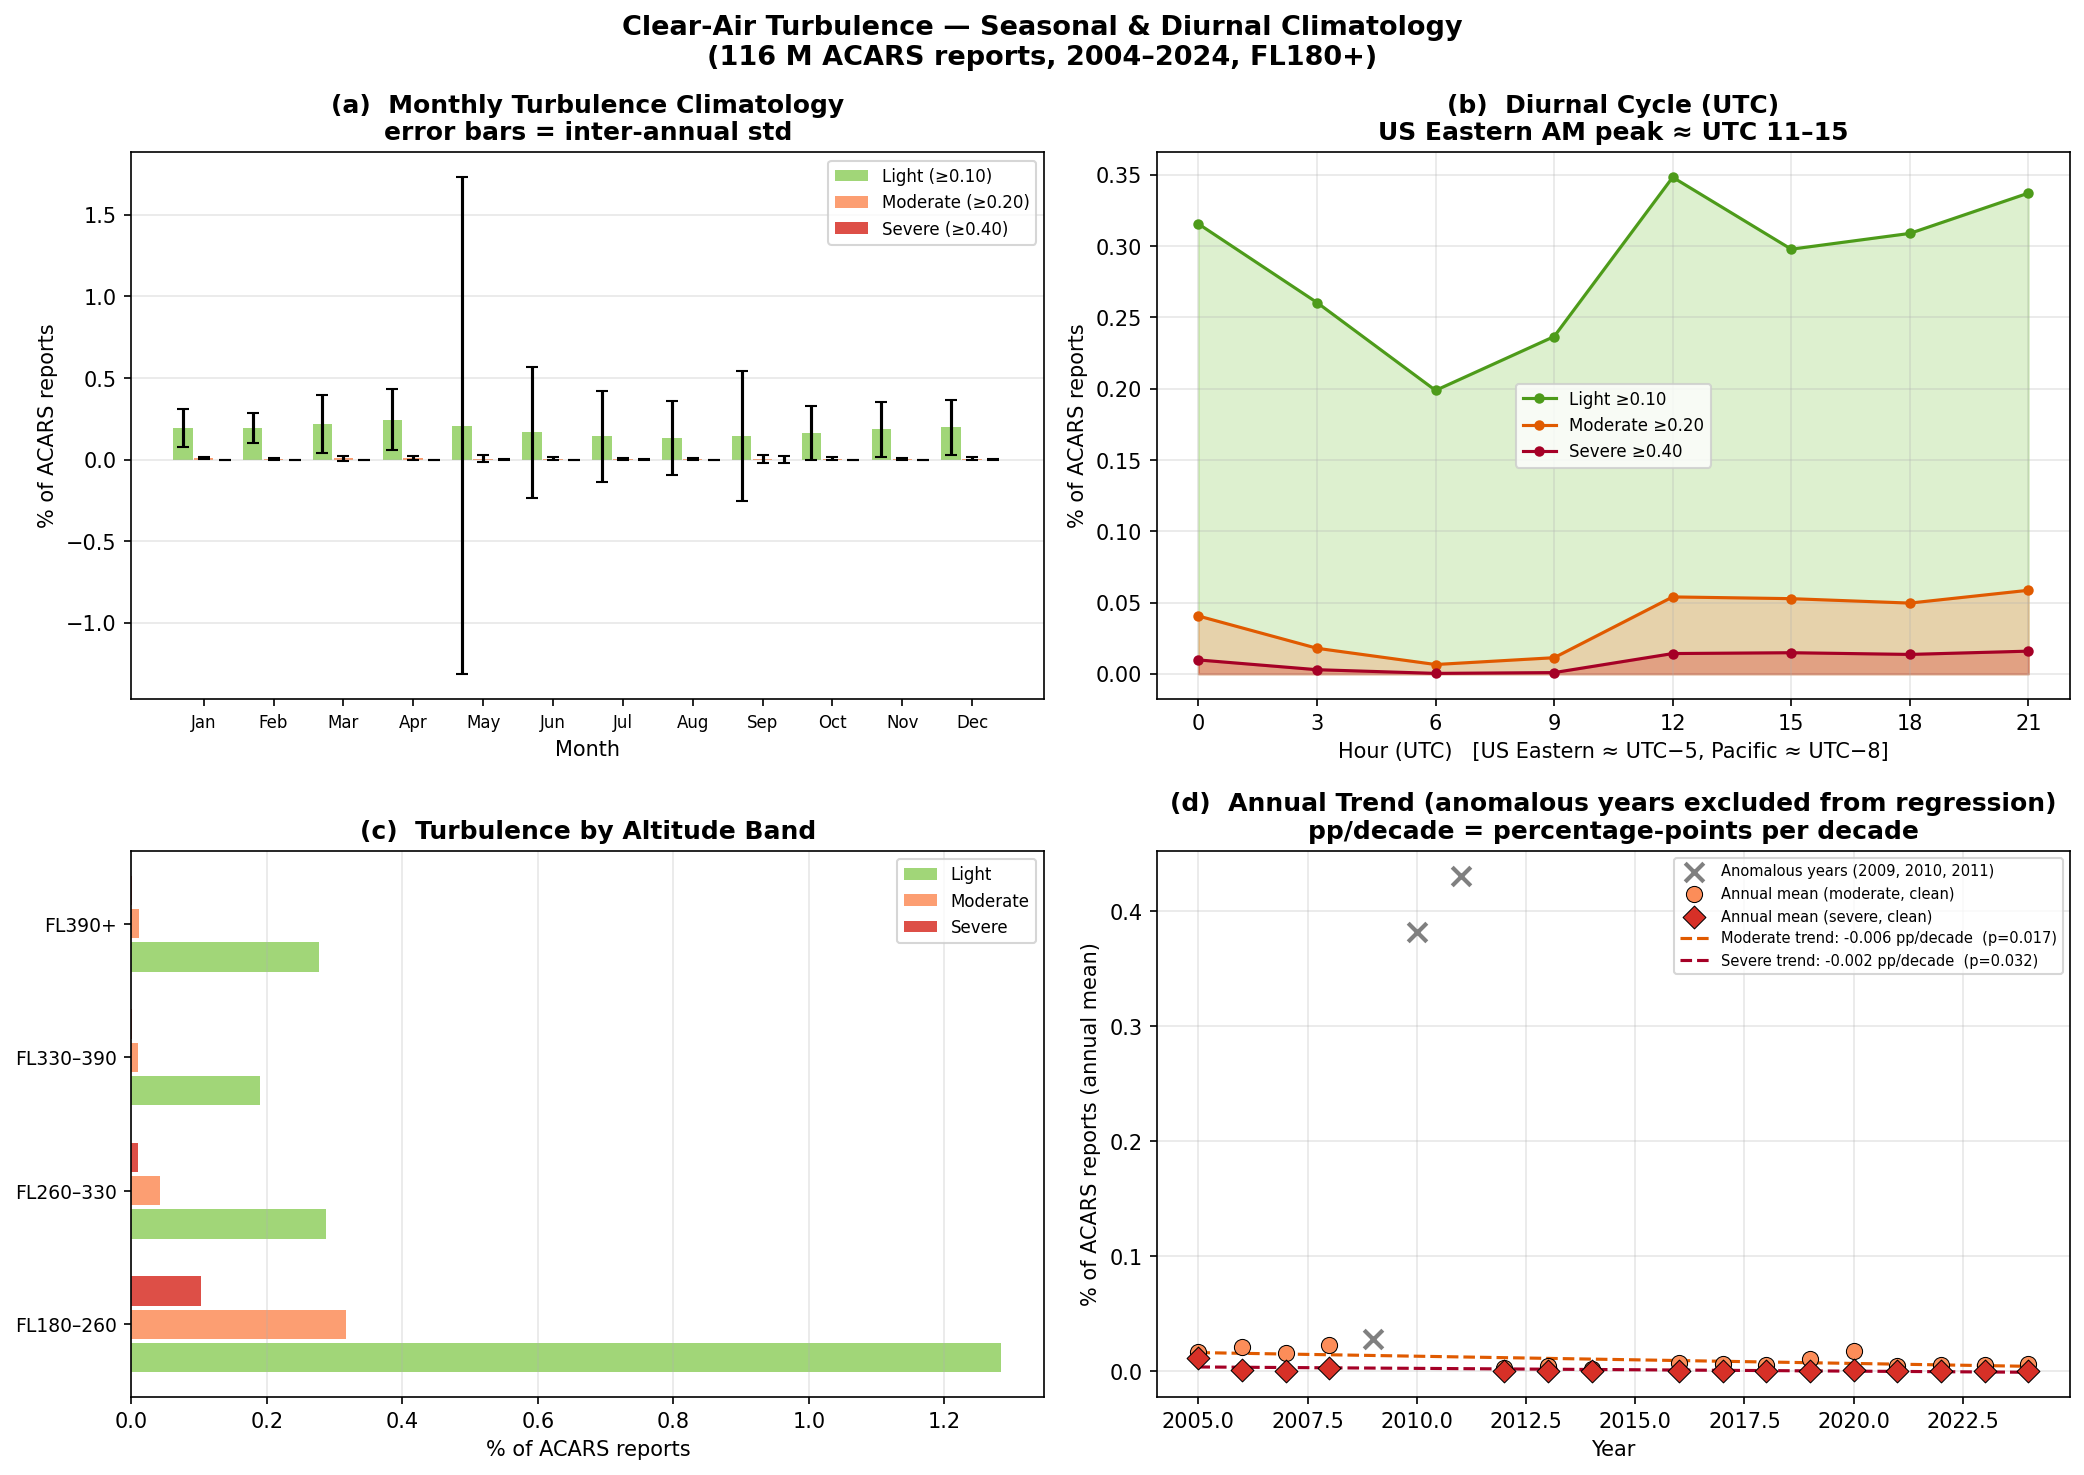
\includegraphics[width=0.88\linewidth]{opt2_climatology.png}
  \caption{Seasonal and diurnal climatology of ACARS turbulence
  (116\,M reports, FL180+). (a)~Monthly climatology with inter-annual
  error bars (January peak); (b)~weak diurnal cycle (21\,UTC peak,
  amplitude 0.052\,pp); (c)~turbulence by altitude band (peak
  FL180--260); (d)~slightly decreasing annual trend, anomalous years
  (grey $\times$) excluded from the regression.}
  \label{fig:climatology}
\end{figure}

\begin{figure}[H]
  \centering
  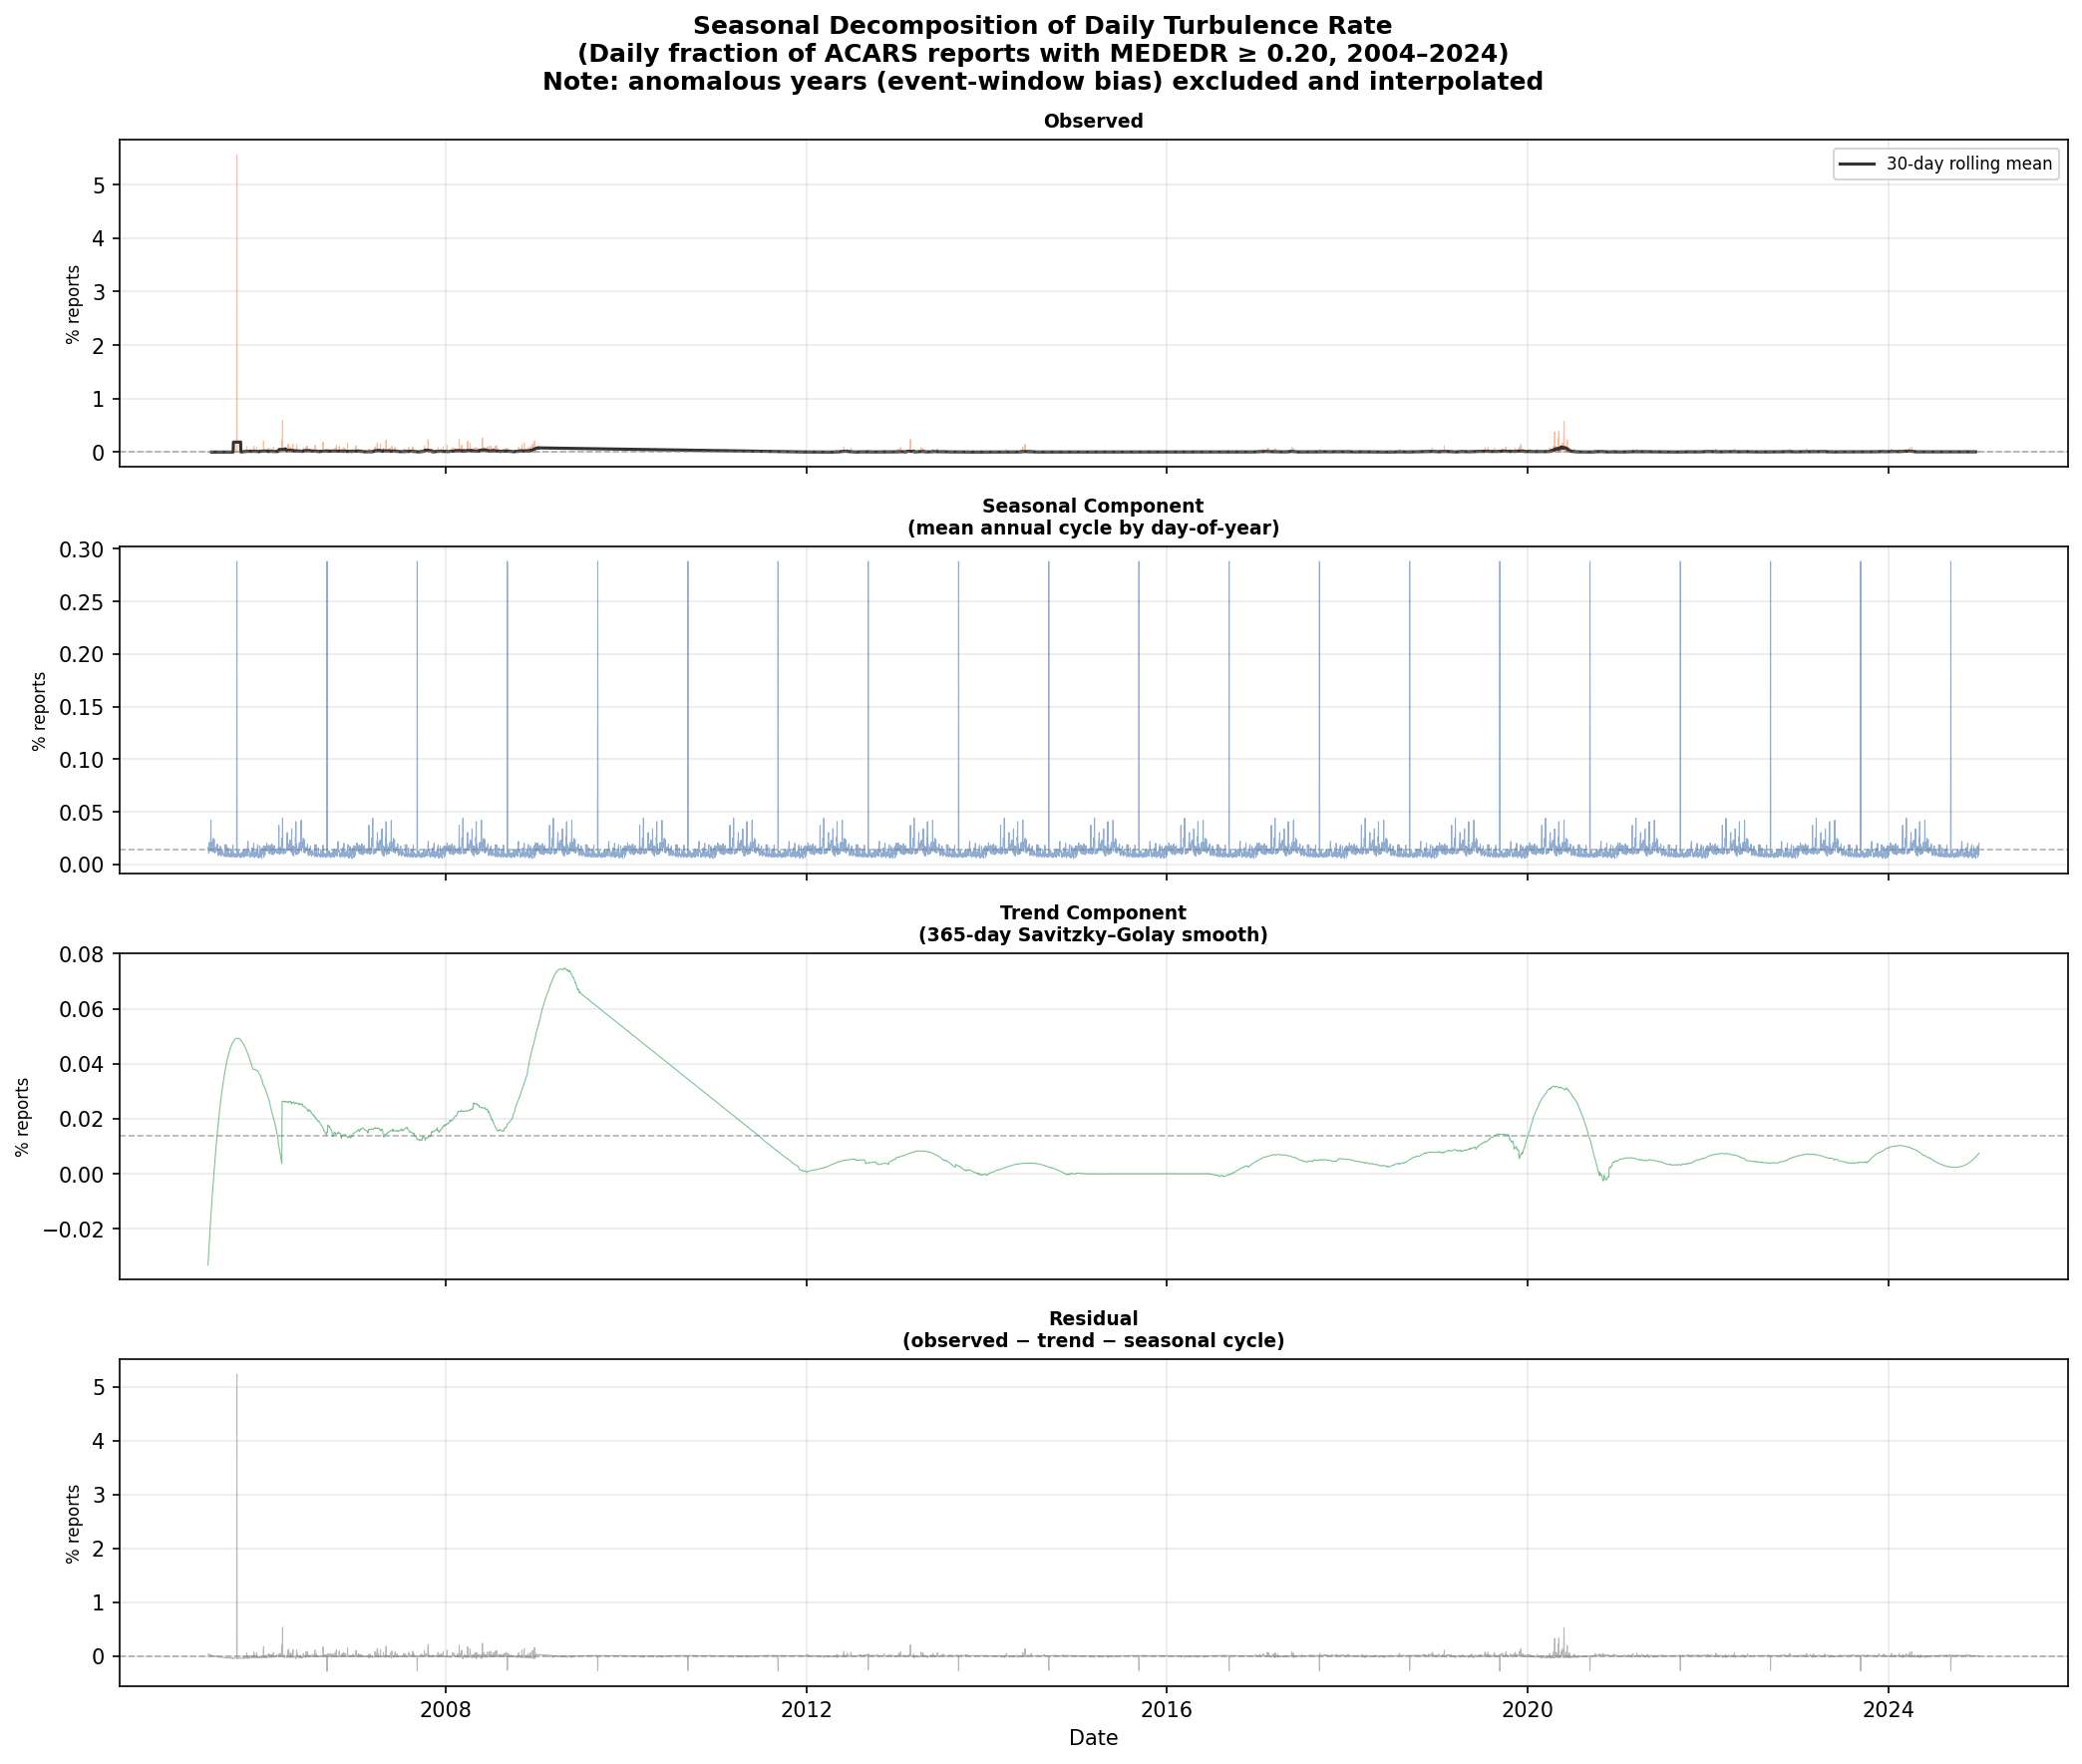
\includegraphics[width=0.88\linewidth]{opt2_decomposition.png}
  \caption{Seasonal decomposition of the daily turbulence rate
  (observed, seasonal, 365-day Savitzky--Golay trend, residual).
  Variance partitions as seasonal 4.8\%, trend 5.4\%, and residual
  (synoptic weather) \textbf{89.8\%}.}
  \label{fig:decomp}
\end{figure}

\begin{figure}[H]
  \centering
  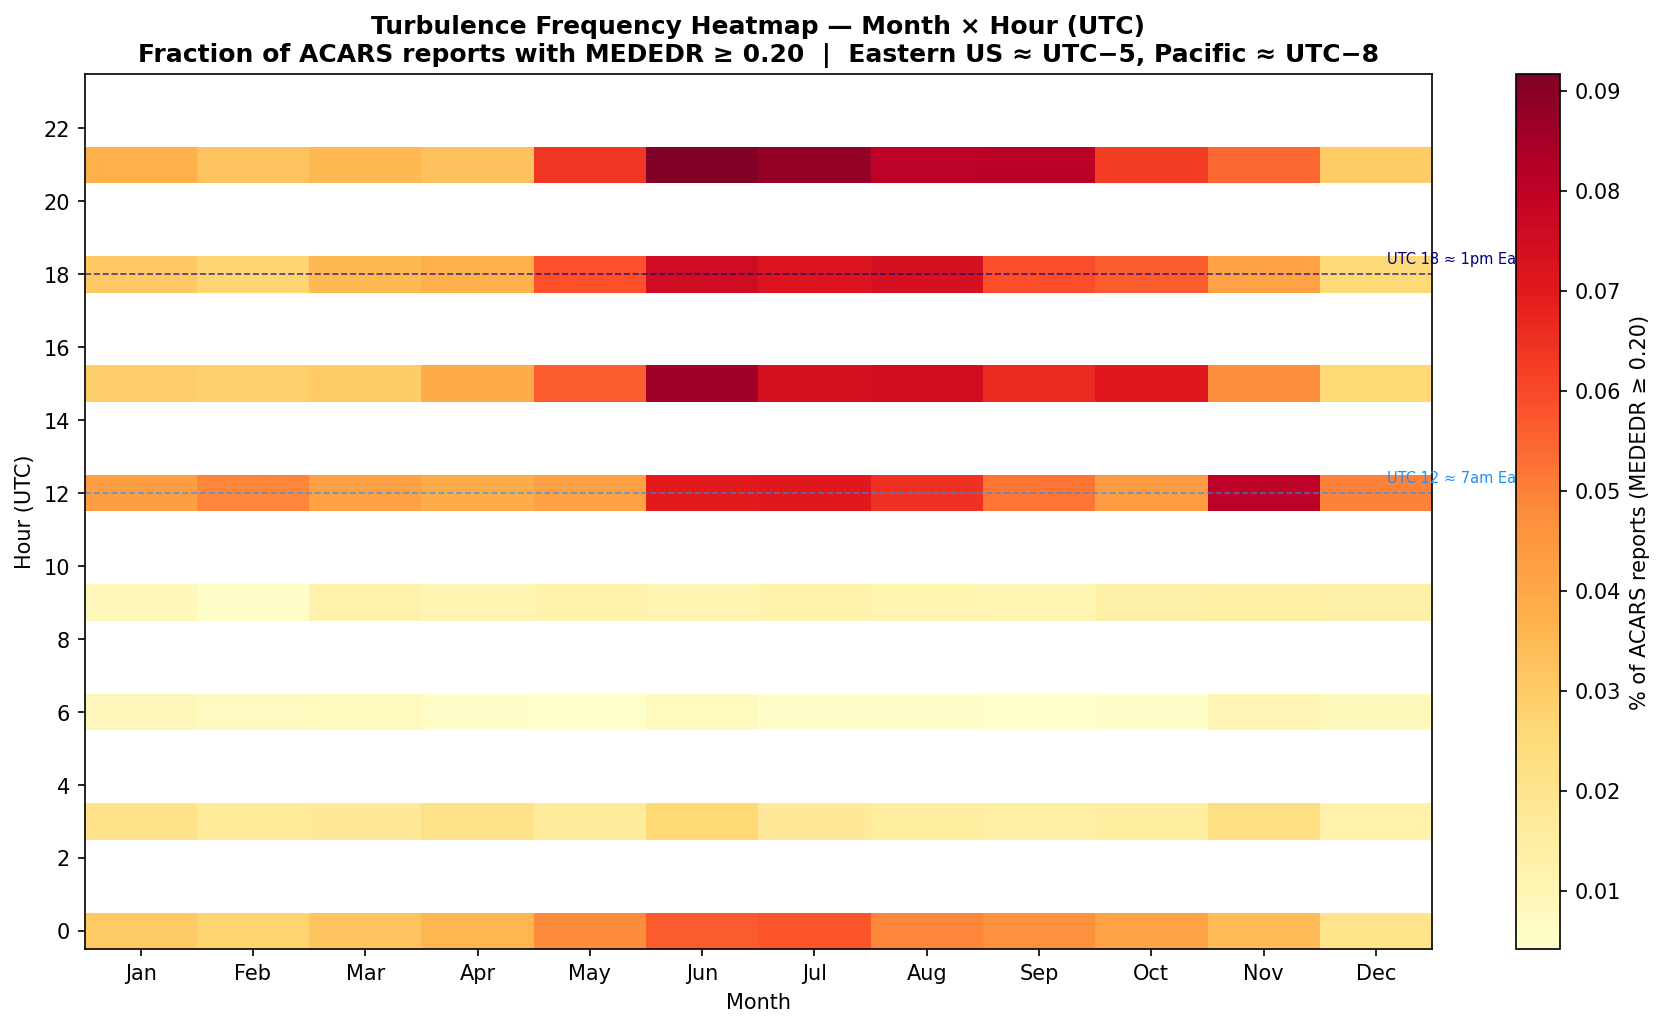
\includegraphics[width=0.88\linewidth]{opt2_heatmap.png}
  \caption{Month $\times$ hour (UTC) turbulence-frequency heatmap. The
  seasonal axis dominates the (very weak) diurnal axis, consistent with
  jet-stream rather than convective forcing.}
  \label{fig:heatmap}
\end{figure}

\subsection{Spectral decomposition: EMD and EEMD}
\label{sec:eda-eemd}
Empirical Mode Decomposition (EMD) adaptively separates a signal into a
small set of \emph{intrinsic mode functions} (IMFs)---quasi-oscillatory
components ordered from the fastest to the slowest timescale---plus a
monotonic residual trend. Unlike a Fourier basis, IMFs need not have a
fixed period: each is a narrowband but amplitude- and
frequency-modulated cycle, which makes EMD well suited to a non-stationary
geophysical record. We ran two complementary decompositions on two
different monthly signals.

\paragraph{EMD of the occurrence rate (Fig.~\ref{fig:emd}).} Applied to
the monthly fraction of reports exceeding moderate, single-trial EMD puts
most energy in the fastest modes: IMF1 (a $\sim$4-month, sub-seasonal
cycle) carries $\approx$37.5\% of the variance and IMF2 (a $\sim$9-month
cycle) $\approx$33.9\%, while \emph{no clean 12-month annual mode}
emerges. Read physically, the month-to-month \emph{rate} of turbulence is
an irregular sub-seasonal oscillation---the rhythm of passing weather
systems---rather than a smooth annual wave.

\paragraph{EEMD of the intensity (Fig.~\ref{fig:eemd}).} Plain EMD can
suffer \emph{mode mixing}, where one IMF blends two timescales. Ensemble
EMD (EEMD) adds many independent noise realisations (here 100 trials,
noise width 0.05) and averages the resulting decompositions, which
populates the timescale axis densely enough to separate the modes
cleanly. Applied to the monthly mean above-threshold \emph{intensity}
(mean $0.269$~\edrunit), EEMD resolves a ladder of cycles---sub-seasonal
($\sim$3--4\,mo), semi-annual to annual ($\sim$7--9\,mo), inter-annual
($\sim$1.5\,yr), multi-year ($\sim$4\,yr, 11.7\%), and decadal
($\sim$8\,yr, 18.8\%)---atop a gentle trend. The notable feature is how
much energy lives at the \emph{low-frequency} end: the multi-year and
decadal cycles together hold roughly a third of the resolved variance.
Per-IMF percentages are method-sensitive (IMFs can be mutually
correlated and need not sum to 100\%), so we read them qualitatively; the
robust statement is that turbulence intensity carries genuine multi-year
and decadal oscillatory energy. The presence of that low-frequency energy
naturally raises whether large-scale climate oscillations co-vary with
turbulence---examined next.

\begin{figure}[H]
  \centering
  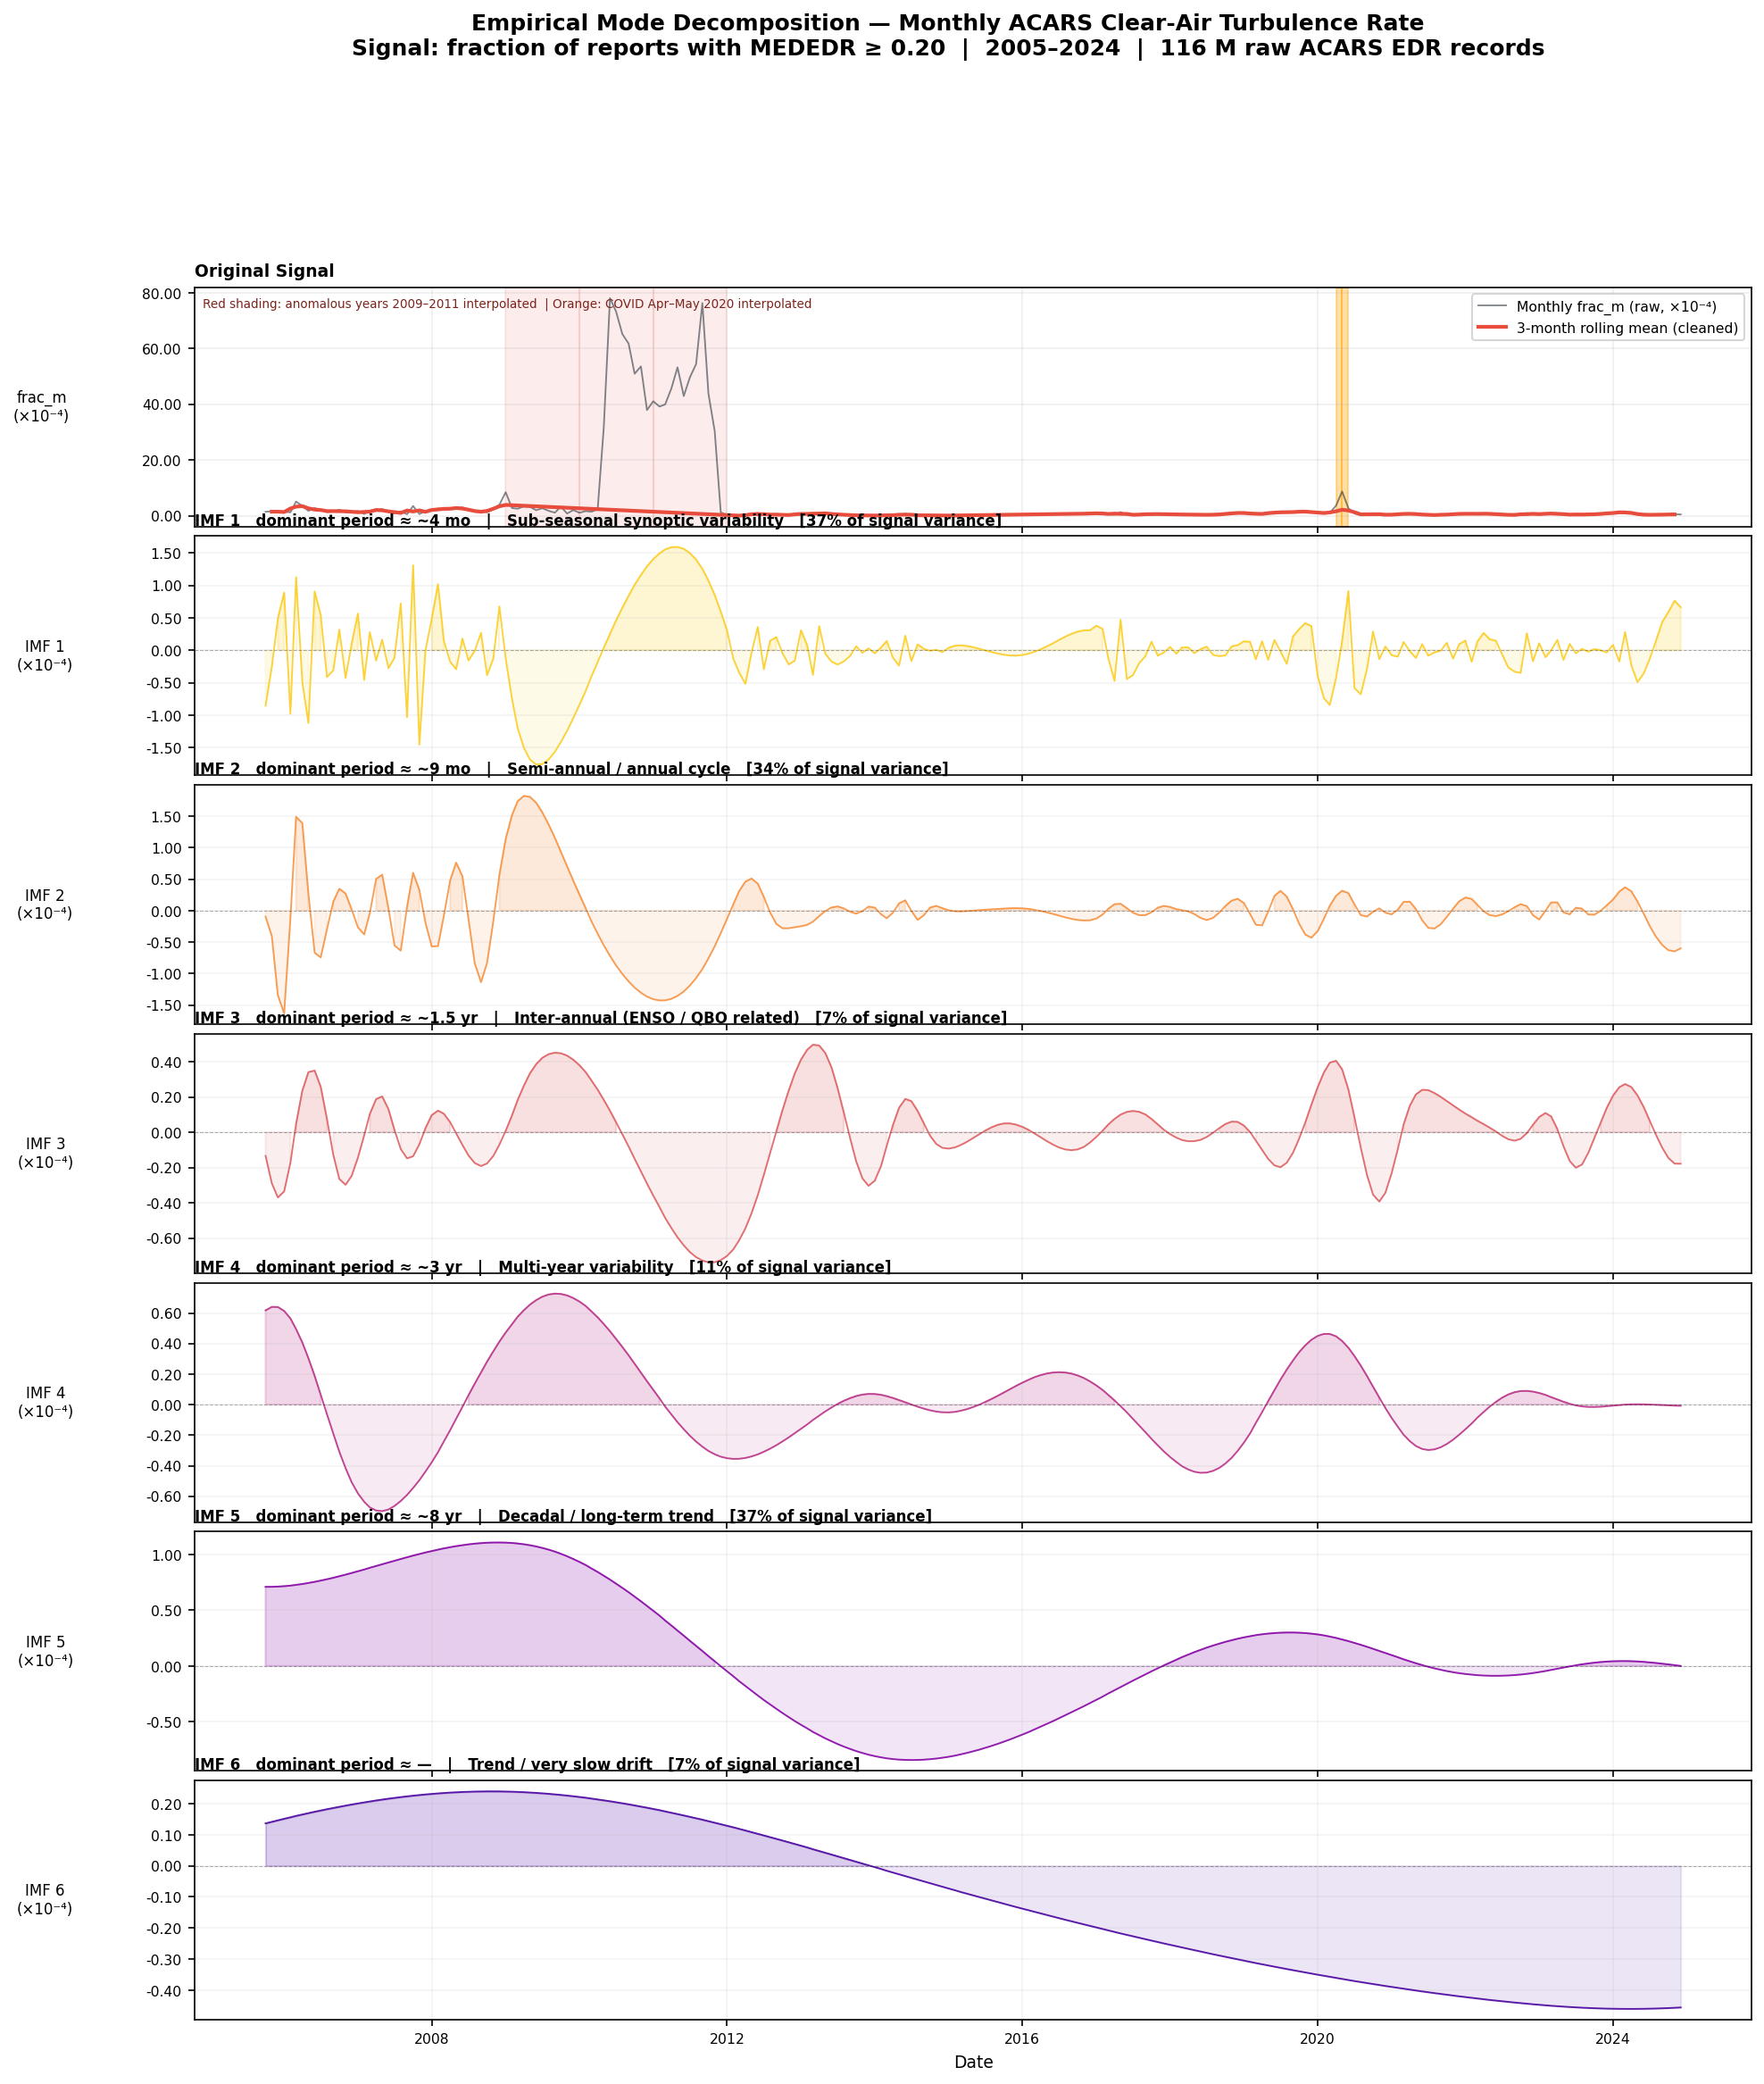
\includegraphics[width=0.88\linewidth]{emd_turbulence.png}
  \caption{EMD of the monthly turbulence \emph{rate}. Sub-seasonal IMF1
  ($\sim$4\,mo, 37.5\%) and IMF2 ($\sim$9\,mo, 33.9\%) dominate and no
  clean annual mode appears: the occurrence rate is an irregular
  sub-seasonal oscillation.}
  \label{fig:emd}
\end{figure}

\begin{figure}[H]
  \centering
  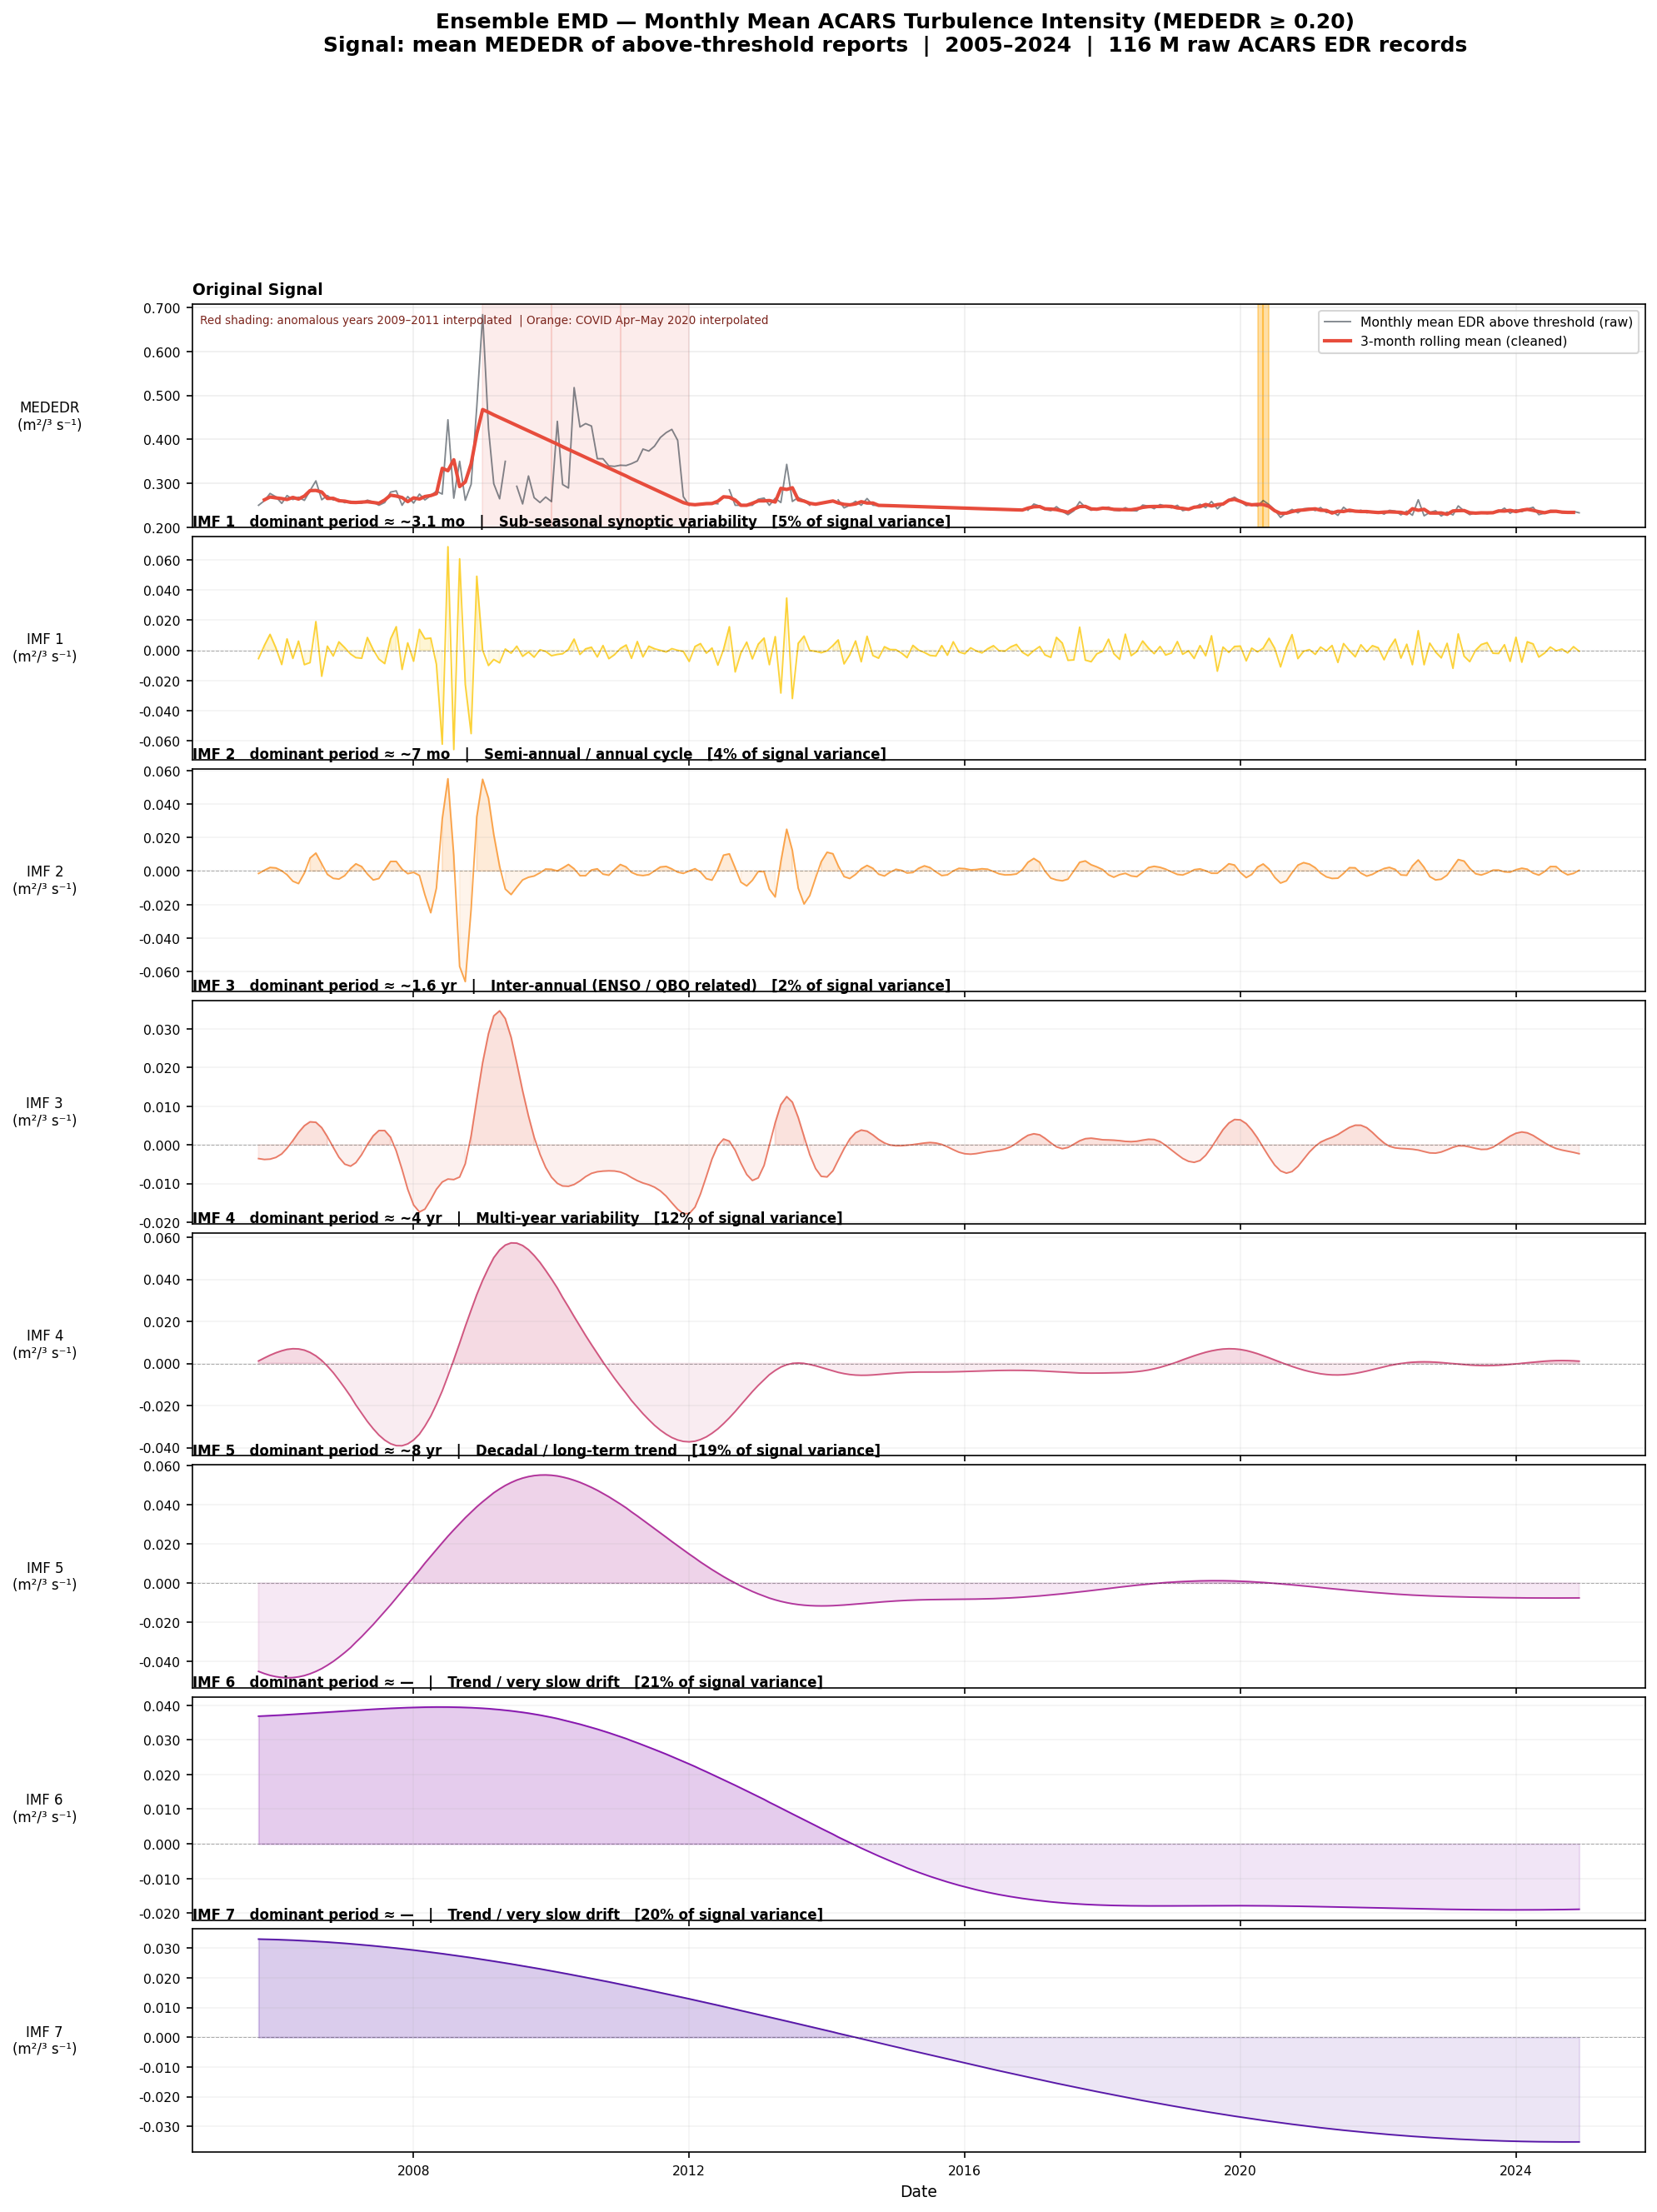
\includegraphics[width=0.88\linewidth]{eemd_turbulence.png}
  \caption{EEMD (100 trials) of the monthly turbulence \emph{intensity}.
  Ensemble averaging separates sub-seasonal through decadal modes,
  exposing prominent multi-year ($\sim$4\,yr) and decadal ($\sim$8\,yr)
  oscillations.}
  \label{fig:eemd}
\end{figure}

\subsection{Climate-index teleconnections}
\label{sec:eda-climate}
We matched each EEMD mode to the climate index nearest its native band
(ONI/ENSO, Ni\~no3.4, QBO, PDO, NAO, AO, MJO) and computed lagged
cross-correlations over $\pm 12$\,months on 170 valid months. Because two
narrowband series correlate by chance, significance was assessed against
\textbf{1000 Fourier phase-randomised surrogates}, and a Hilbert
amplitude-envelope test asked whether turbulence variability
\emph{strengthens} in a given climate phase (Fig.~\ref{fig:climate-amp}).
Phase correlations are modest ($|r|=0.14$--$0.42$) and \textbf{none are
significant} ($p>0.05$) under surrogates; large envelope correlations
(e.g.\ PDO $+0.98$) are inflated by autocorrelation and too few
independent cycles in a 20-year record. Lead/lag signs are mostly
\emph{negative} (turbulence leading the index), the signature of a shared
trend rather than a predictive teleconnection. \textbf{The data therefore
show no statistically robust monthly climate teleconnection for North
American CAT}: the low-frequency EEMD energy is real, but it does not
track any single named oscillation.

\begin{figure}[H]
  \centering
  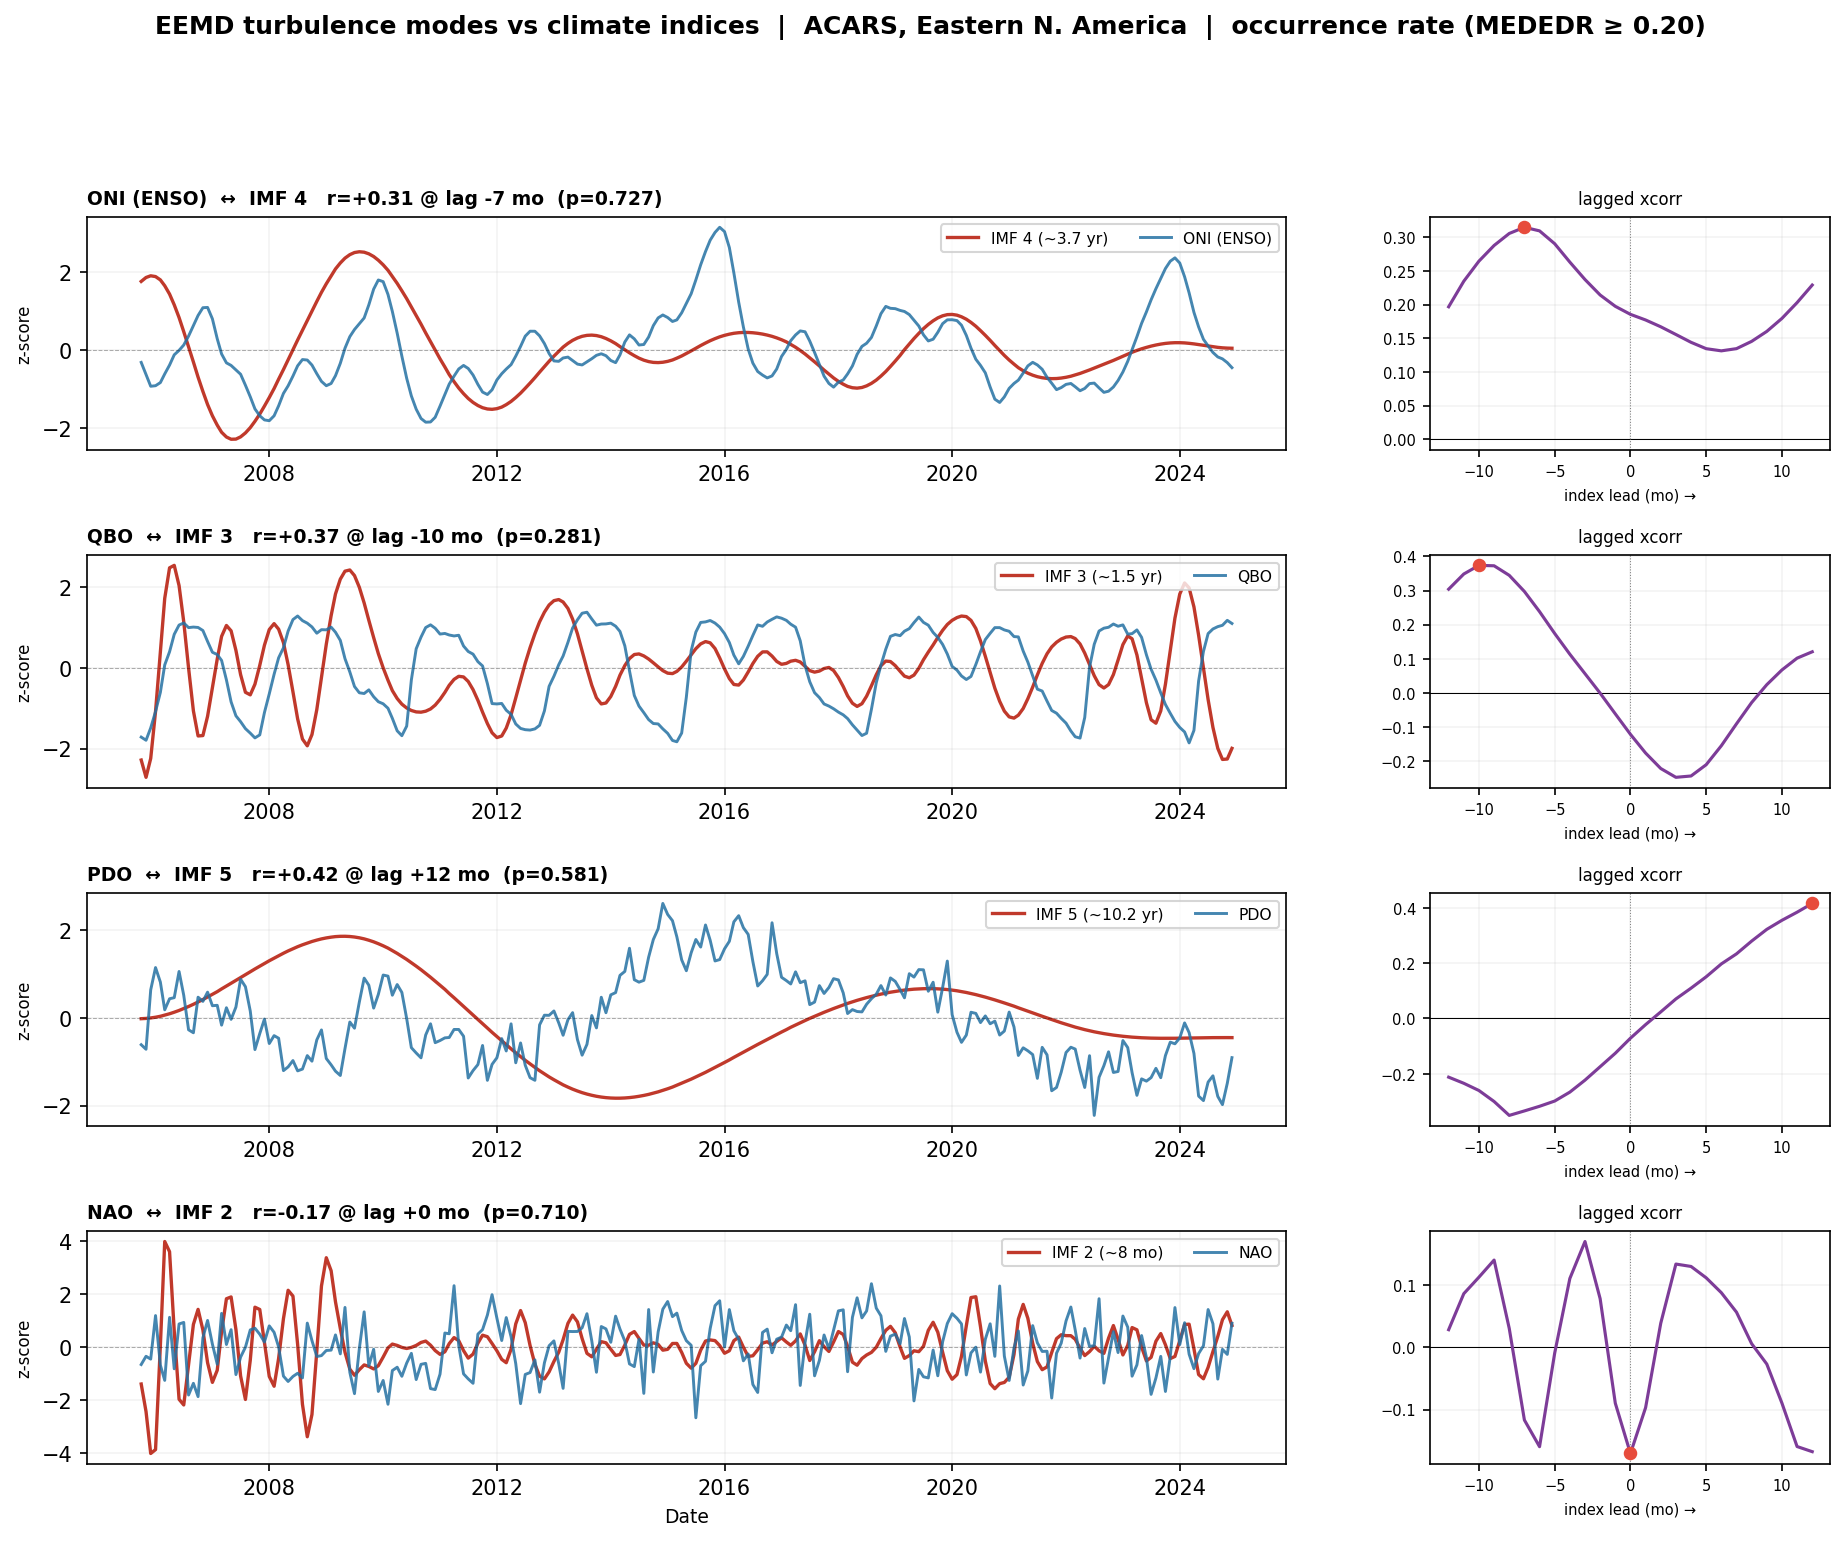
\includegraphics[width=0.88\linewidth]{climate_indices.png}
  \caption{Lagged cross-correlations of EEMD turbulence modes against
  climate indices (ONI, QBO, PDO, NAO). All correlations are
  non-significant under 1000 phase-randomised surrogates ($p>0.05$).}
  \label{fig:climate}
\end{figure}

\begin{figure}[H]
  \centering
  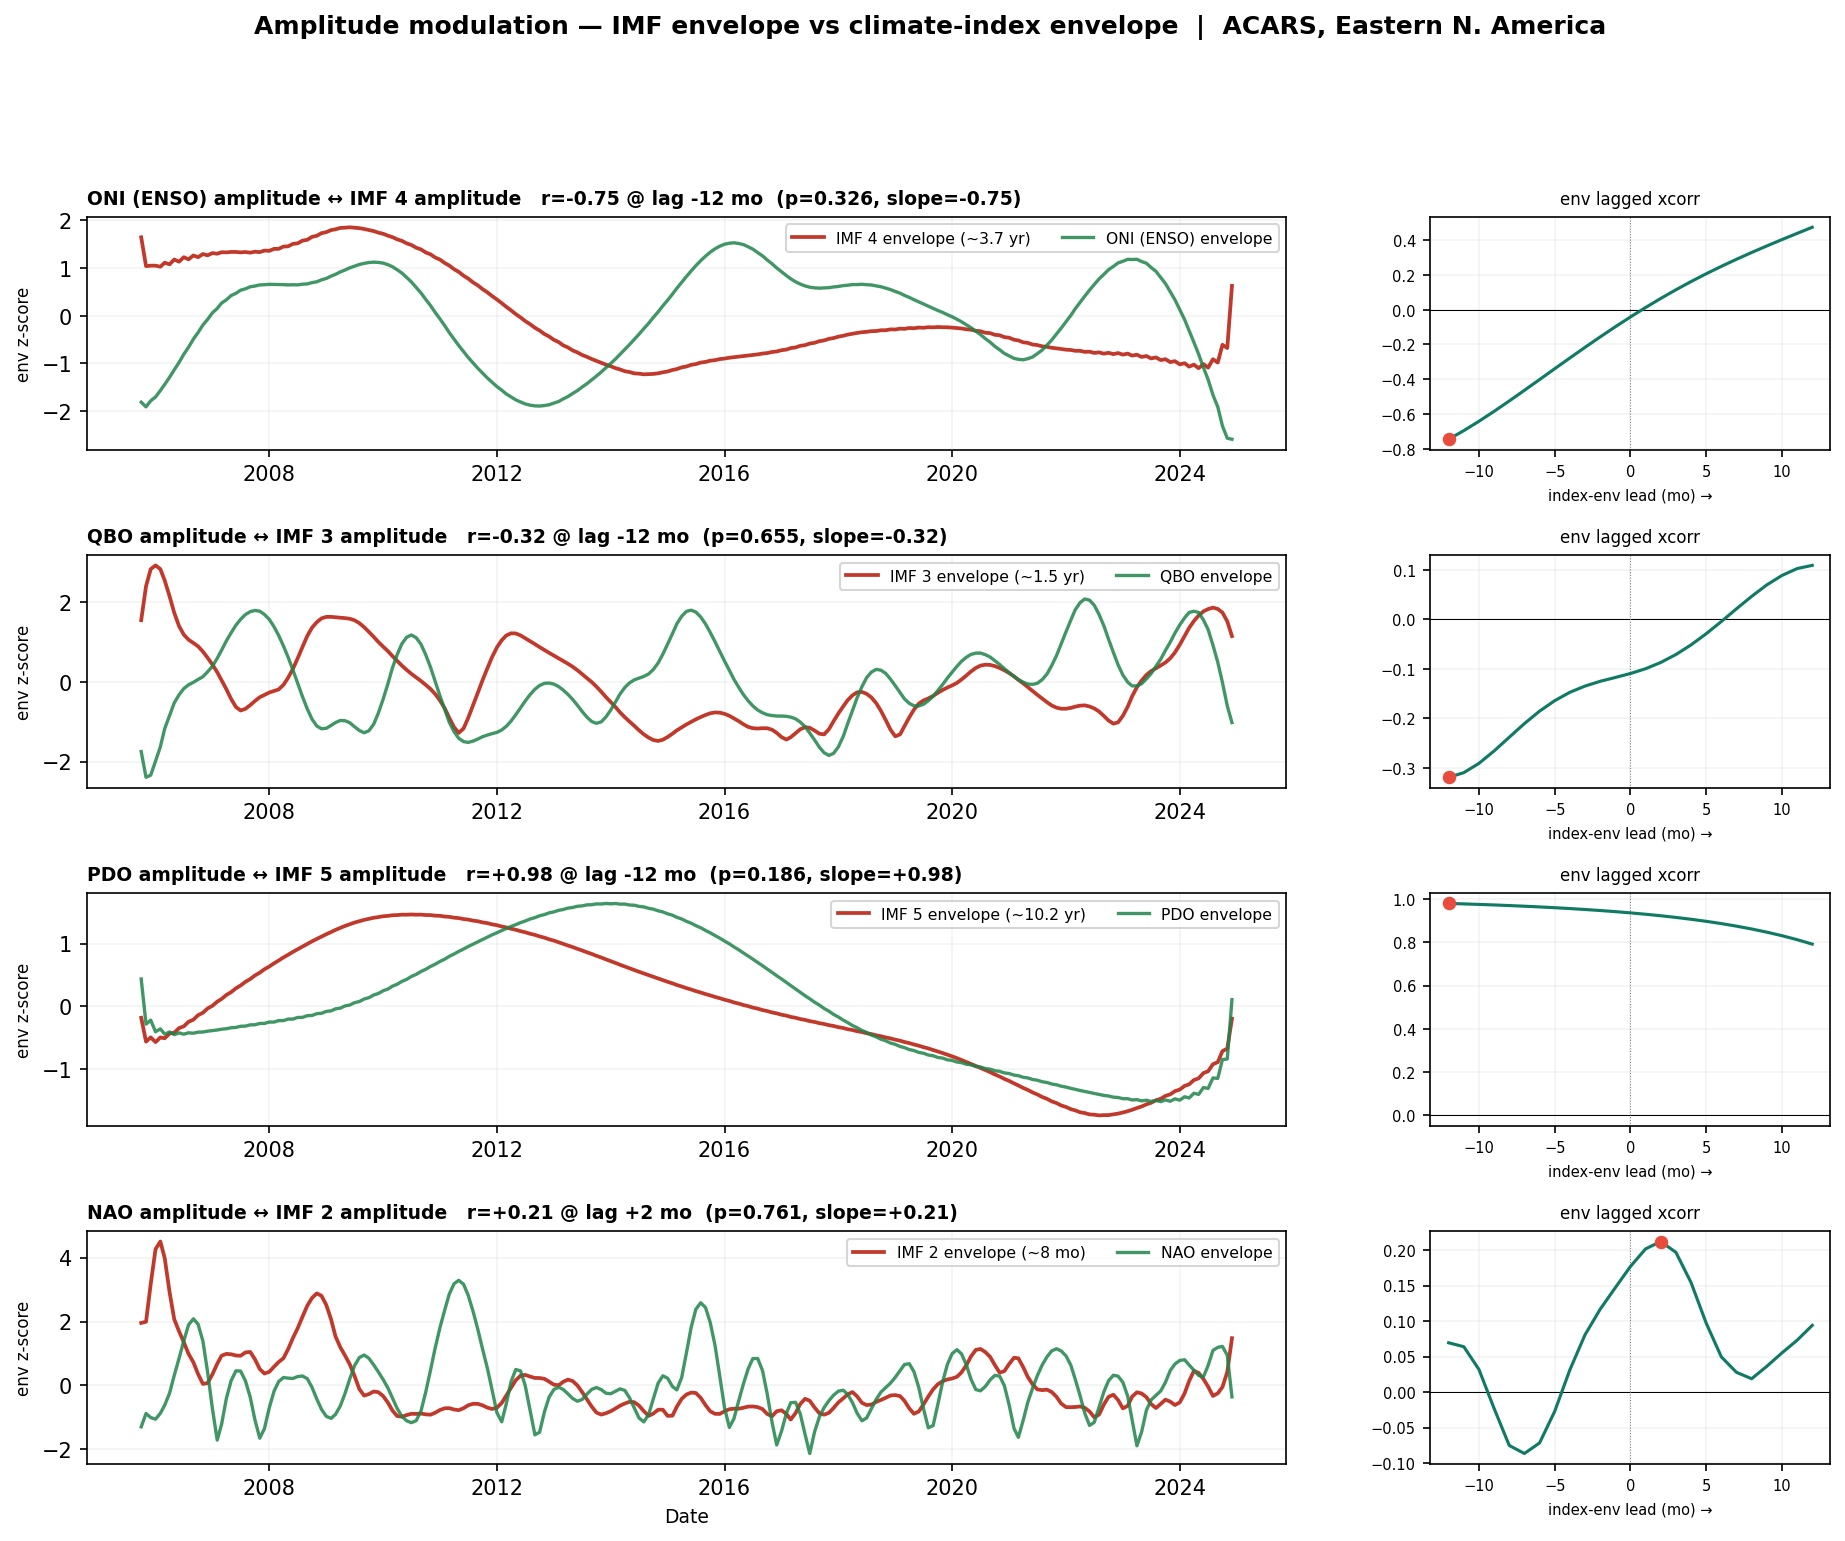
\includegraphics[width=0.88\linewidth]{climate_amplitude.png}
  \caption{Amplitude-modulation (Hilbert-envelope) test. Apparent
  envelope correlations (e.g.\ PDO, $r=+0.98$) are driven by
  autocorrelation and the small number of multi-year cycles
  ($p=0.19$, n.s.), not a real teleconnection.}
  \label{fig:climate-amp}
\end{figure}

\subsection{Regional spatial distribution (ADS-B)}
\label{sec:eda-regional}
Using OpenSky ADS-B state vectors we built a turbulence proxy---intra-hour
standard deviation of vertical rate $>1.5$\,m\,s$^{-1}$, calibrated to
$\mathrm{MEDEDR}\geq 0.20$ following \citet{kim2021,sharman2016}---and
mapped month~$\times$~hour encounter rates across 15 global aviation
regions (dateline-aware; FL180+ cruise; $\geq$5 obs/aircraft-hour;
Fig.~\ref{fig:regional}). Encounter rates vary markedly by region and
season: mid-latitude regions threaded by the polar jet (North America,
the North Atlantic, East Asia) show the strongest winter maxima, while
tropical regions are comparatively flat. Geography and season, in short,
both structure where and when turbulence is encountered.

\begin{figure}[H]
  \centering
  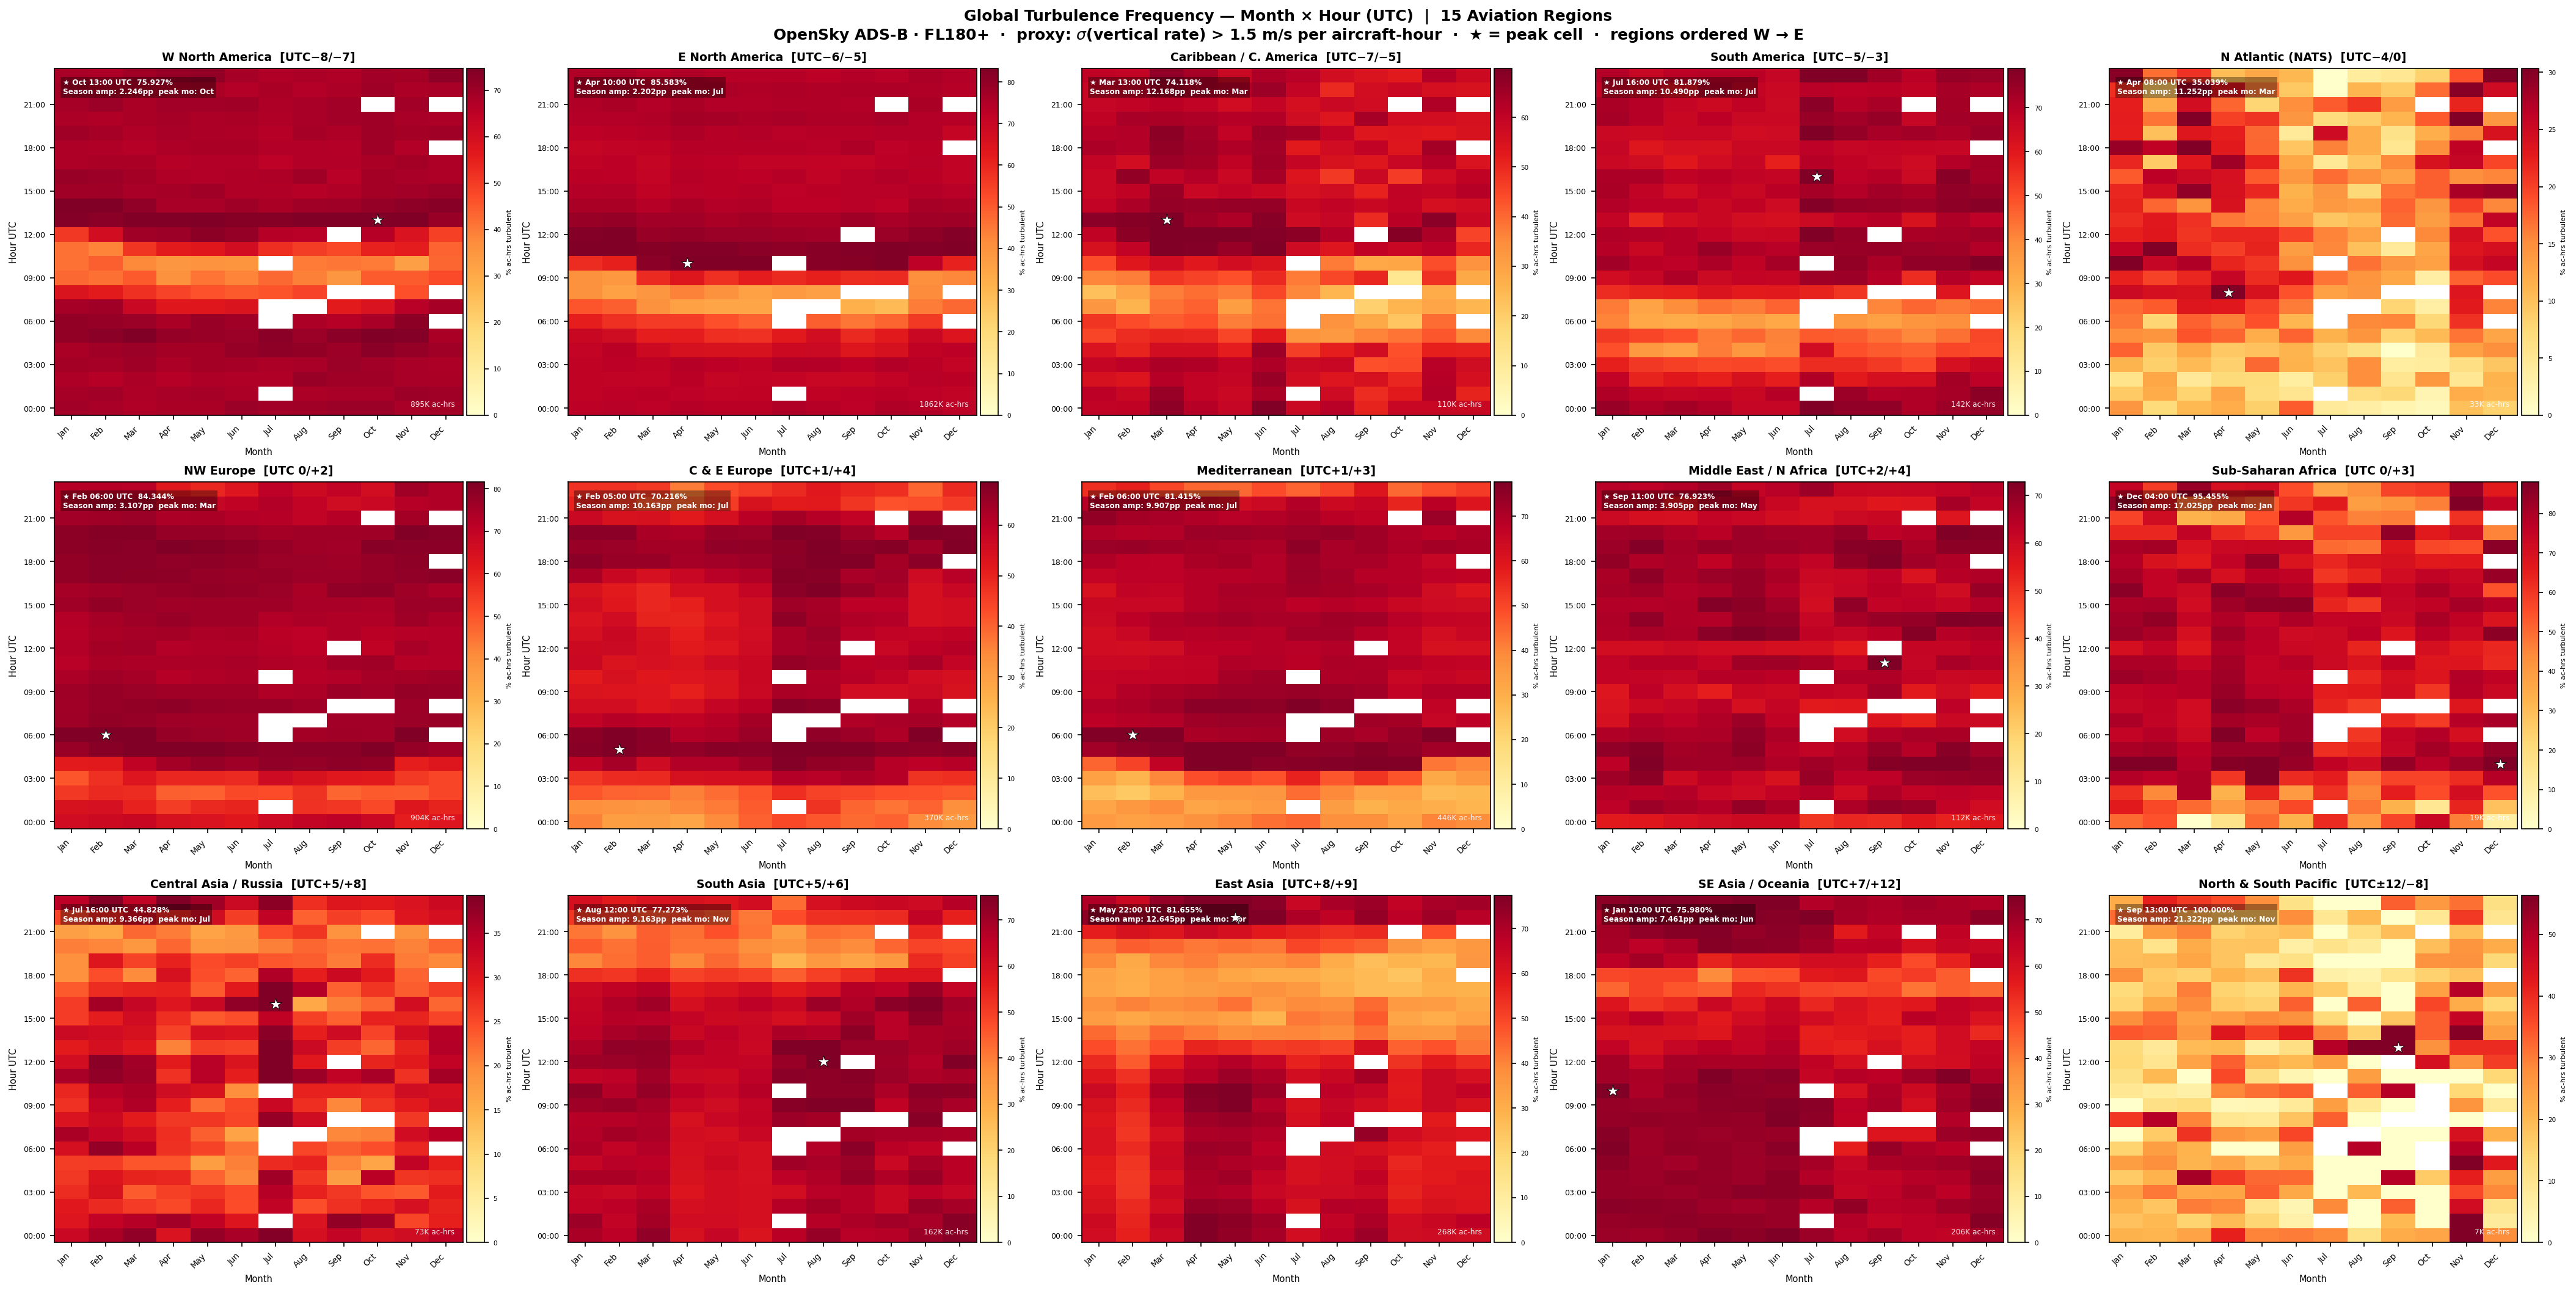
\includegraphics[width=0.88\linewidth]{regional_heatmaps.png}
  \caption{Month $\times$ hour (UTC) turbulence-proxy heatmaps for 15
  global aviation regions from OpenSky ADS-B (vertical-rate variance
  proxy, std$(w)>1.5$\,m\,s$^{-1}$). Peak cells ($\star$), seasonal
  amplitude, and sample sizes are annotated per region; regions below
  200 aircraft-hours are flagged insufficient.}
  \label{fig:regional}
\end{figure}

\subsection{Satellite TB $\leftrightarrow$ EDR cross-correlation}
\label{sec:eda-sat}
On the 64 satellite-covered events (431 lag-0 pairs), Spearman
correlations against hourly mean EDR are: mean TB $r=-0.27$ ($p<0.001$),
maximum TB $r=-0.20$ ($p<0.001$), minimum TB $r=-0.09$ (n.s.), and TB
spatial spread $\approx 0$ (n.s.). The strongest \emph{forward} predictor
is mean TB at $+2$\,h ($r=-0.31$): colder cloud tops precede turbulence,
implying a $\sim$2-hour lead in convective cases
(Figs.~\ref{fig:sat-lag}--\ref{fig:sat-ts}). The off-trend outliers in
the scatter (Fig.~\ref{fig:sat-scatter}) are precisely the severe
clear-sky events with no cold cloud: the satellite signal is carried by
post-2017 moderate/convective cases and is \textbf{blind to severe jet
CAT}, which by definition has no cloud signature.

\begin{figure}[H]
  \centering
  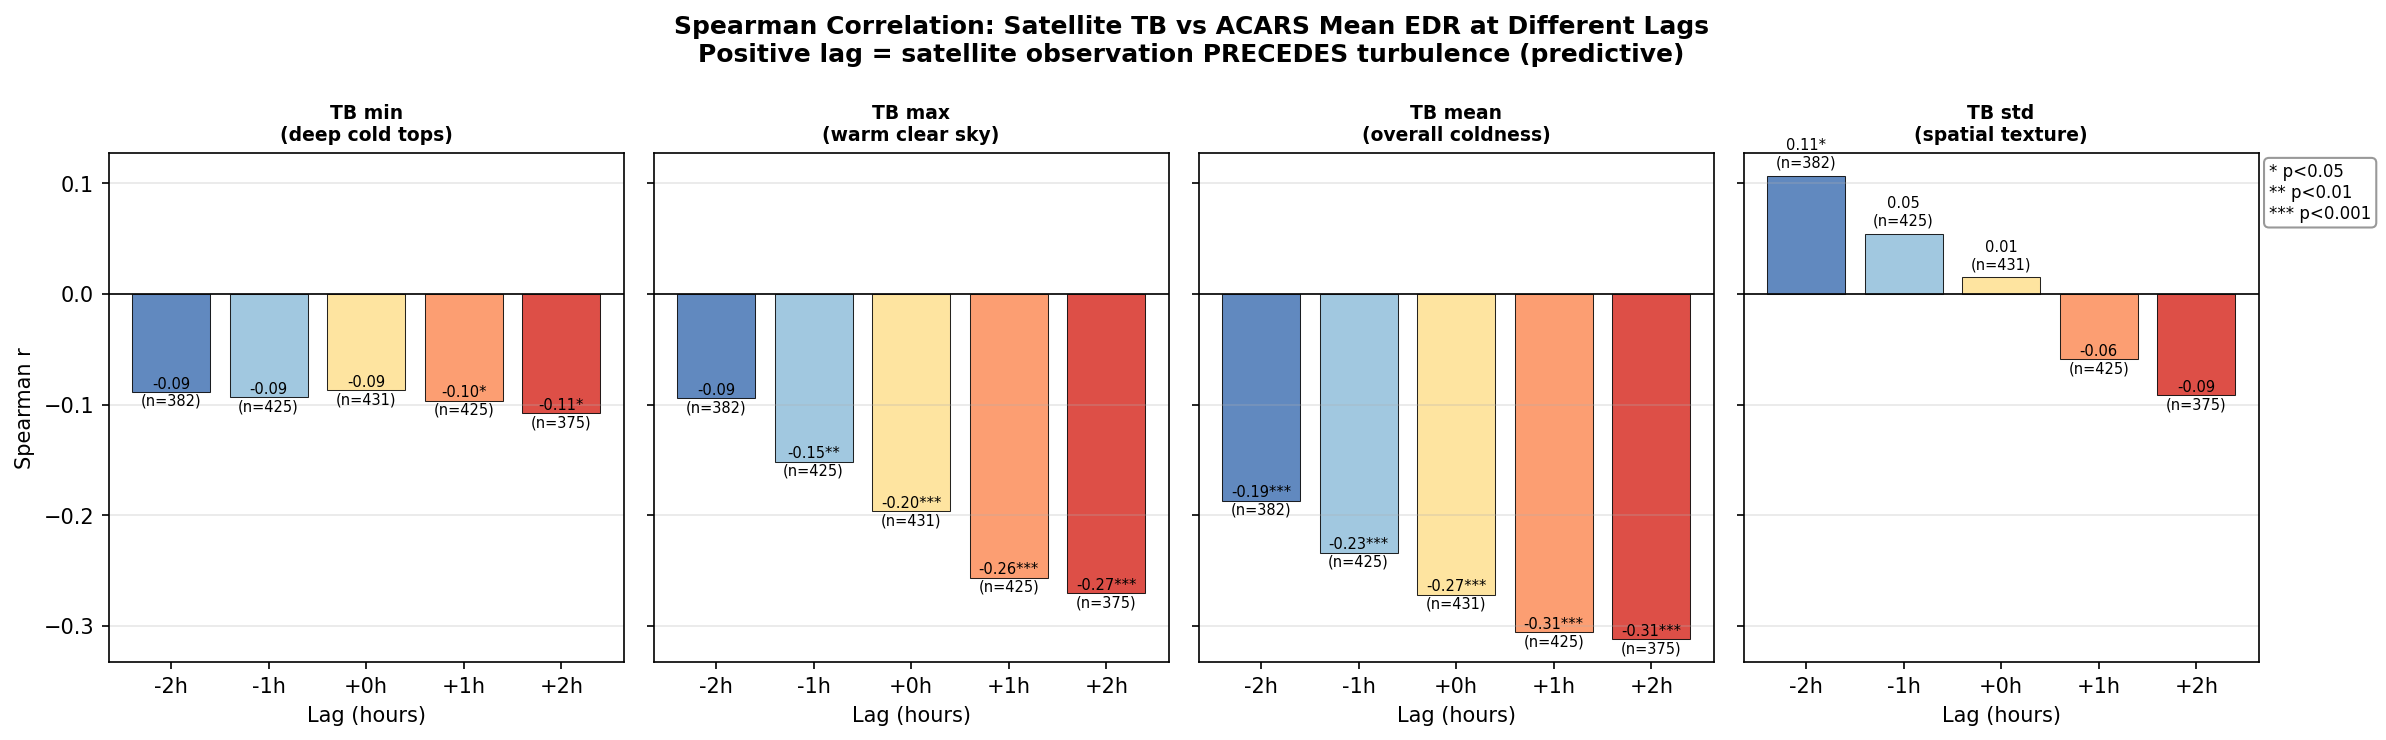
\includegraphics[width=0.88\linewidth]{opt5_lag_correlations.png}
  \caption{Spearman correlation of satellite brightness-temperature
  statistics with ACARS mean EDR at lags $-2$ to $+2$\,h. Positive lag =
  satellite precedes turbulence; mean TB at $+2$\,h gives $r=-0.31$.}
  \label{fig:sat-lag}
\end{figure}

\begin{figure}[H]
  \centering
  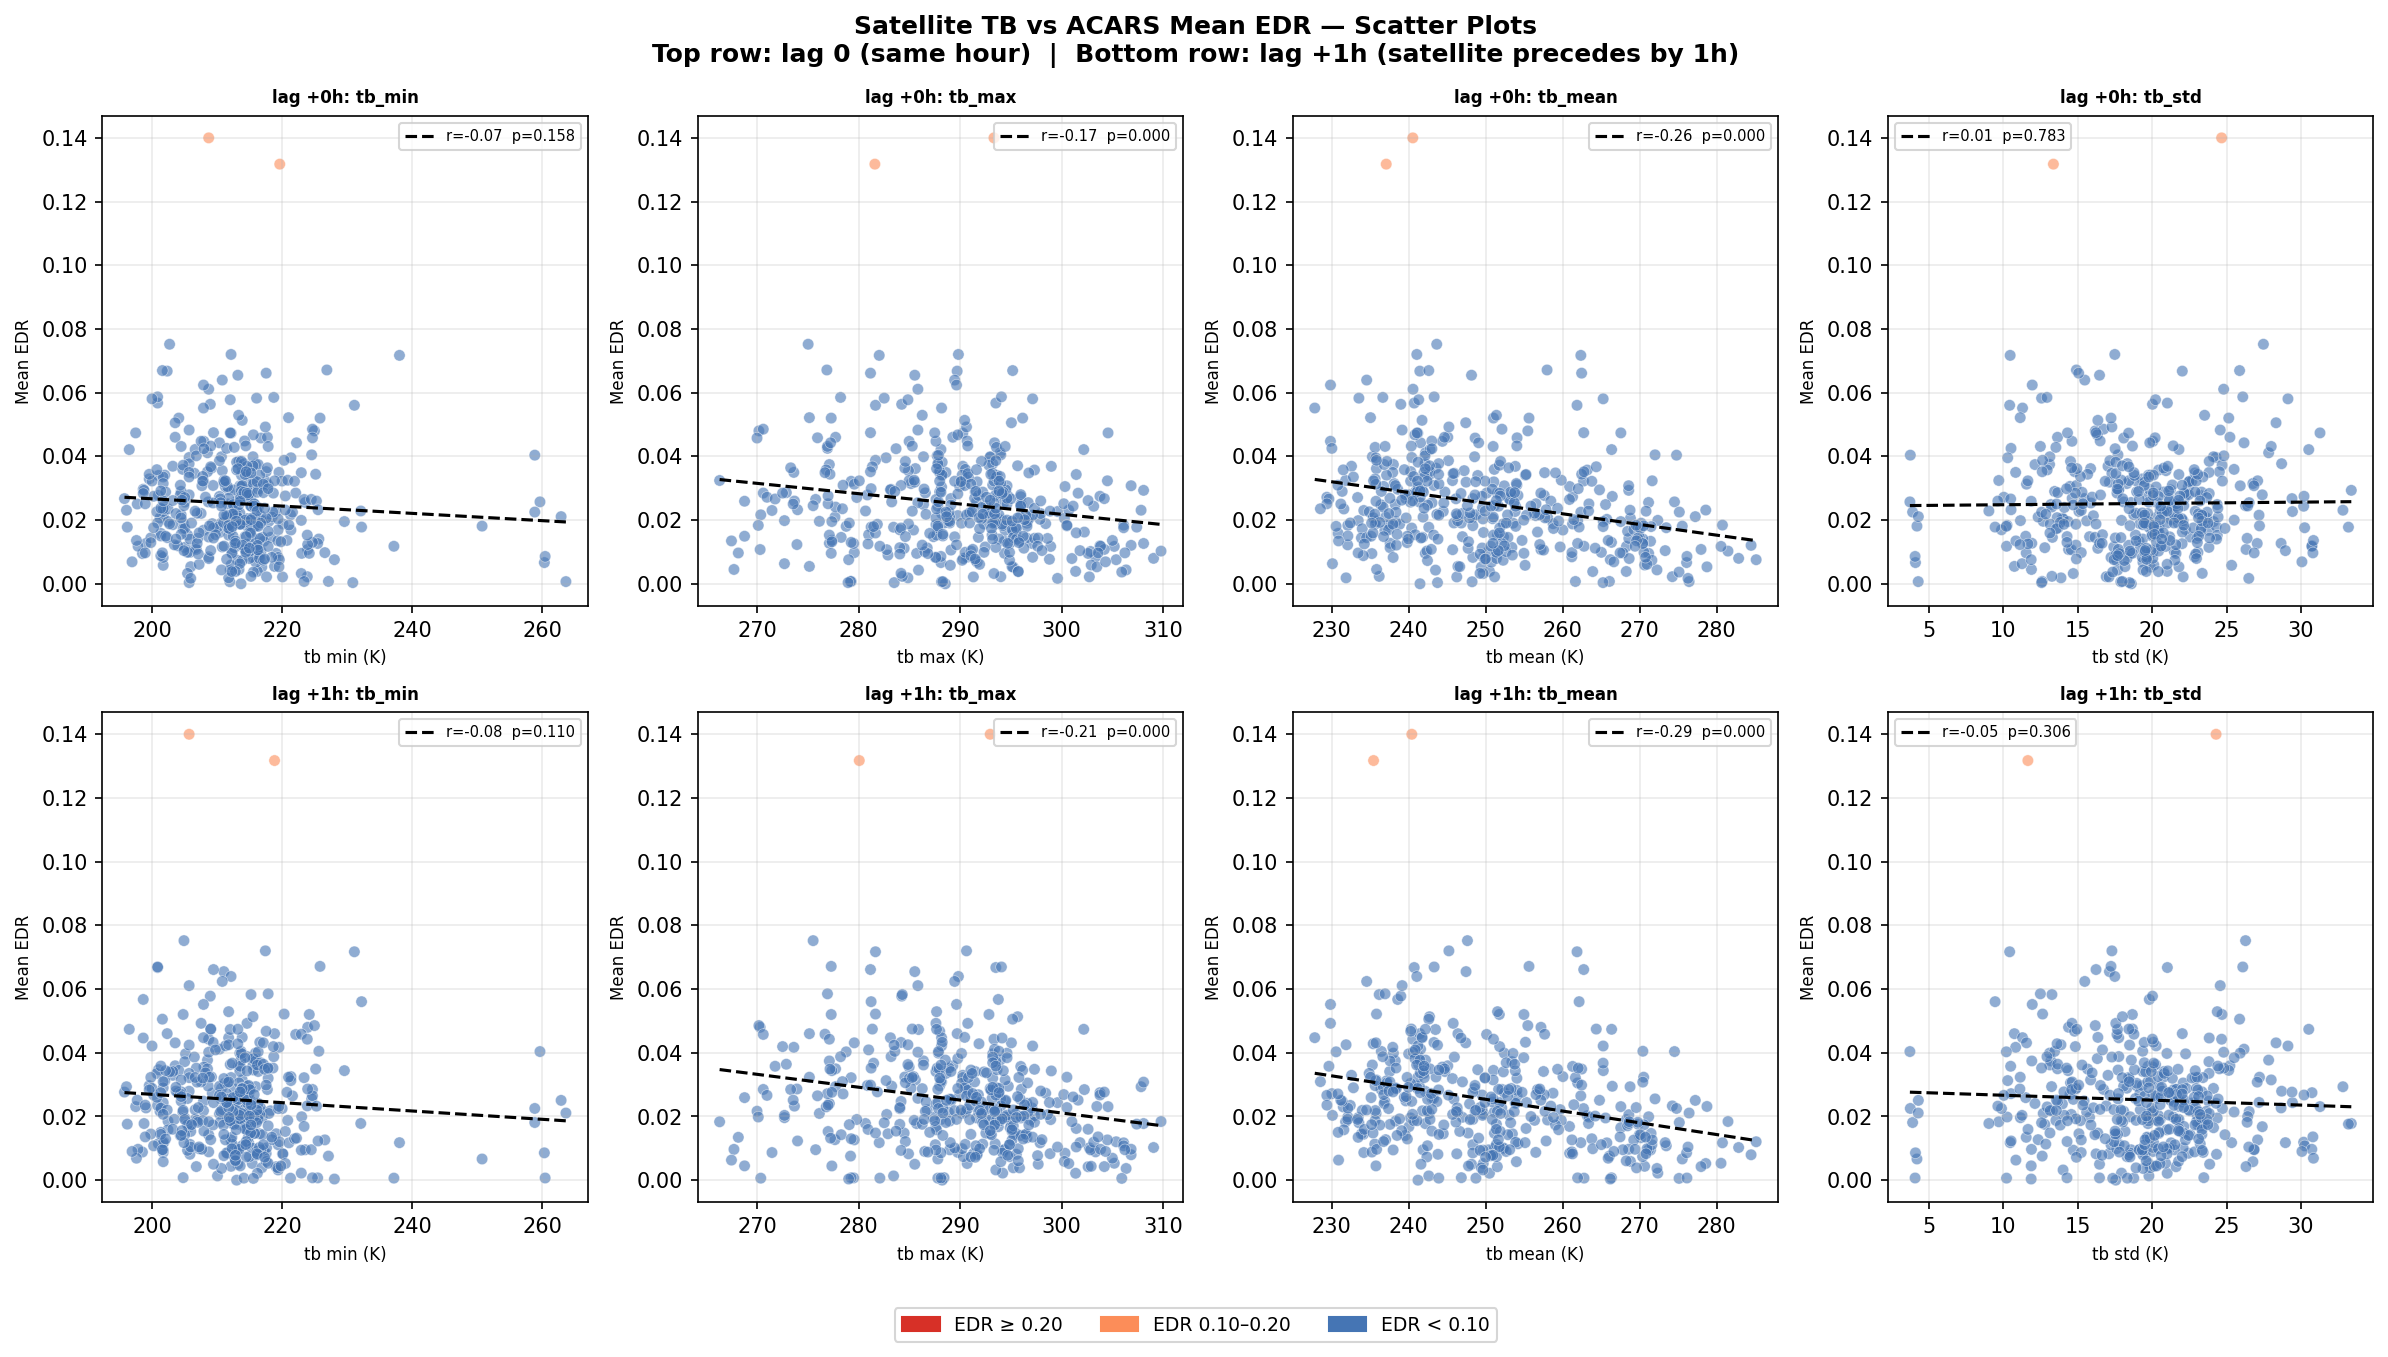
\includegraphics[width=0.88\linewidth]{opt5_scatter_tb_edr.png}
  \caption{Satellite TB vs.\ ACARS mean EDR scatter at lag 0 (top) and
  lag $+1$\,h (bottom). Colder mean/maximum TB associates with higher
  EDR; severe clear-sky events (no cold cloud) are the off-trend
  outliers.}
  \label{fig:sat-scatter}
\end{figure}

\begin{figure}[H]
  \centering
  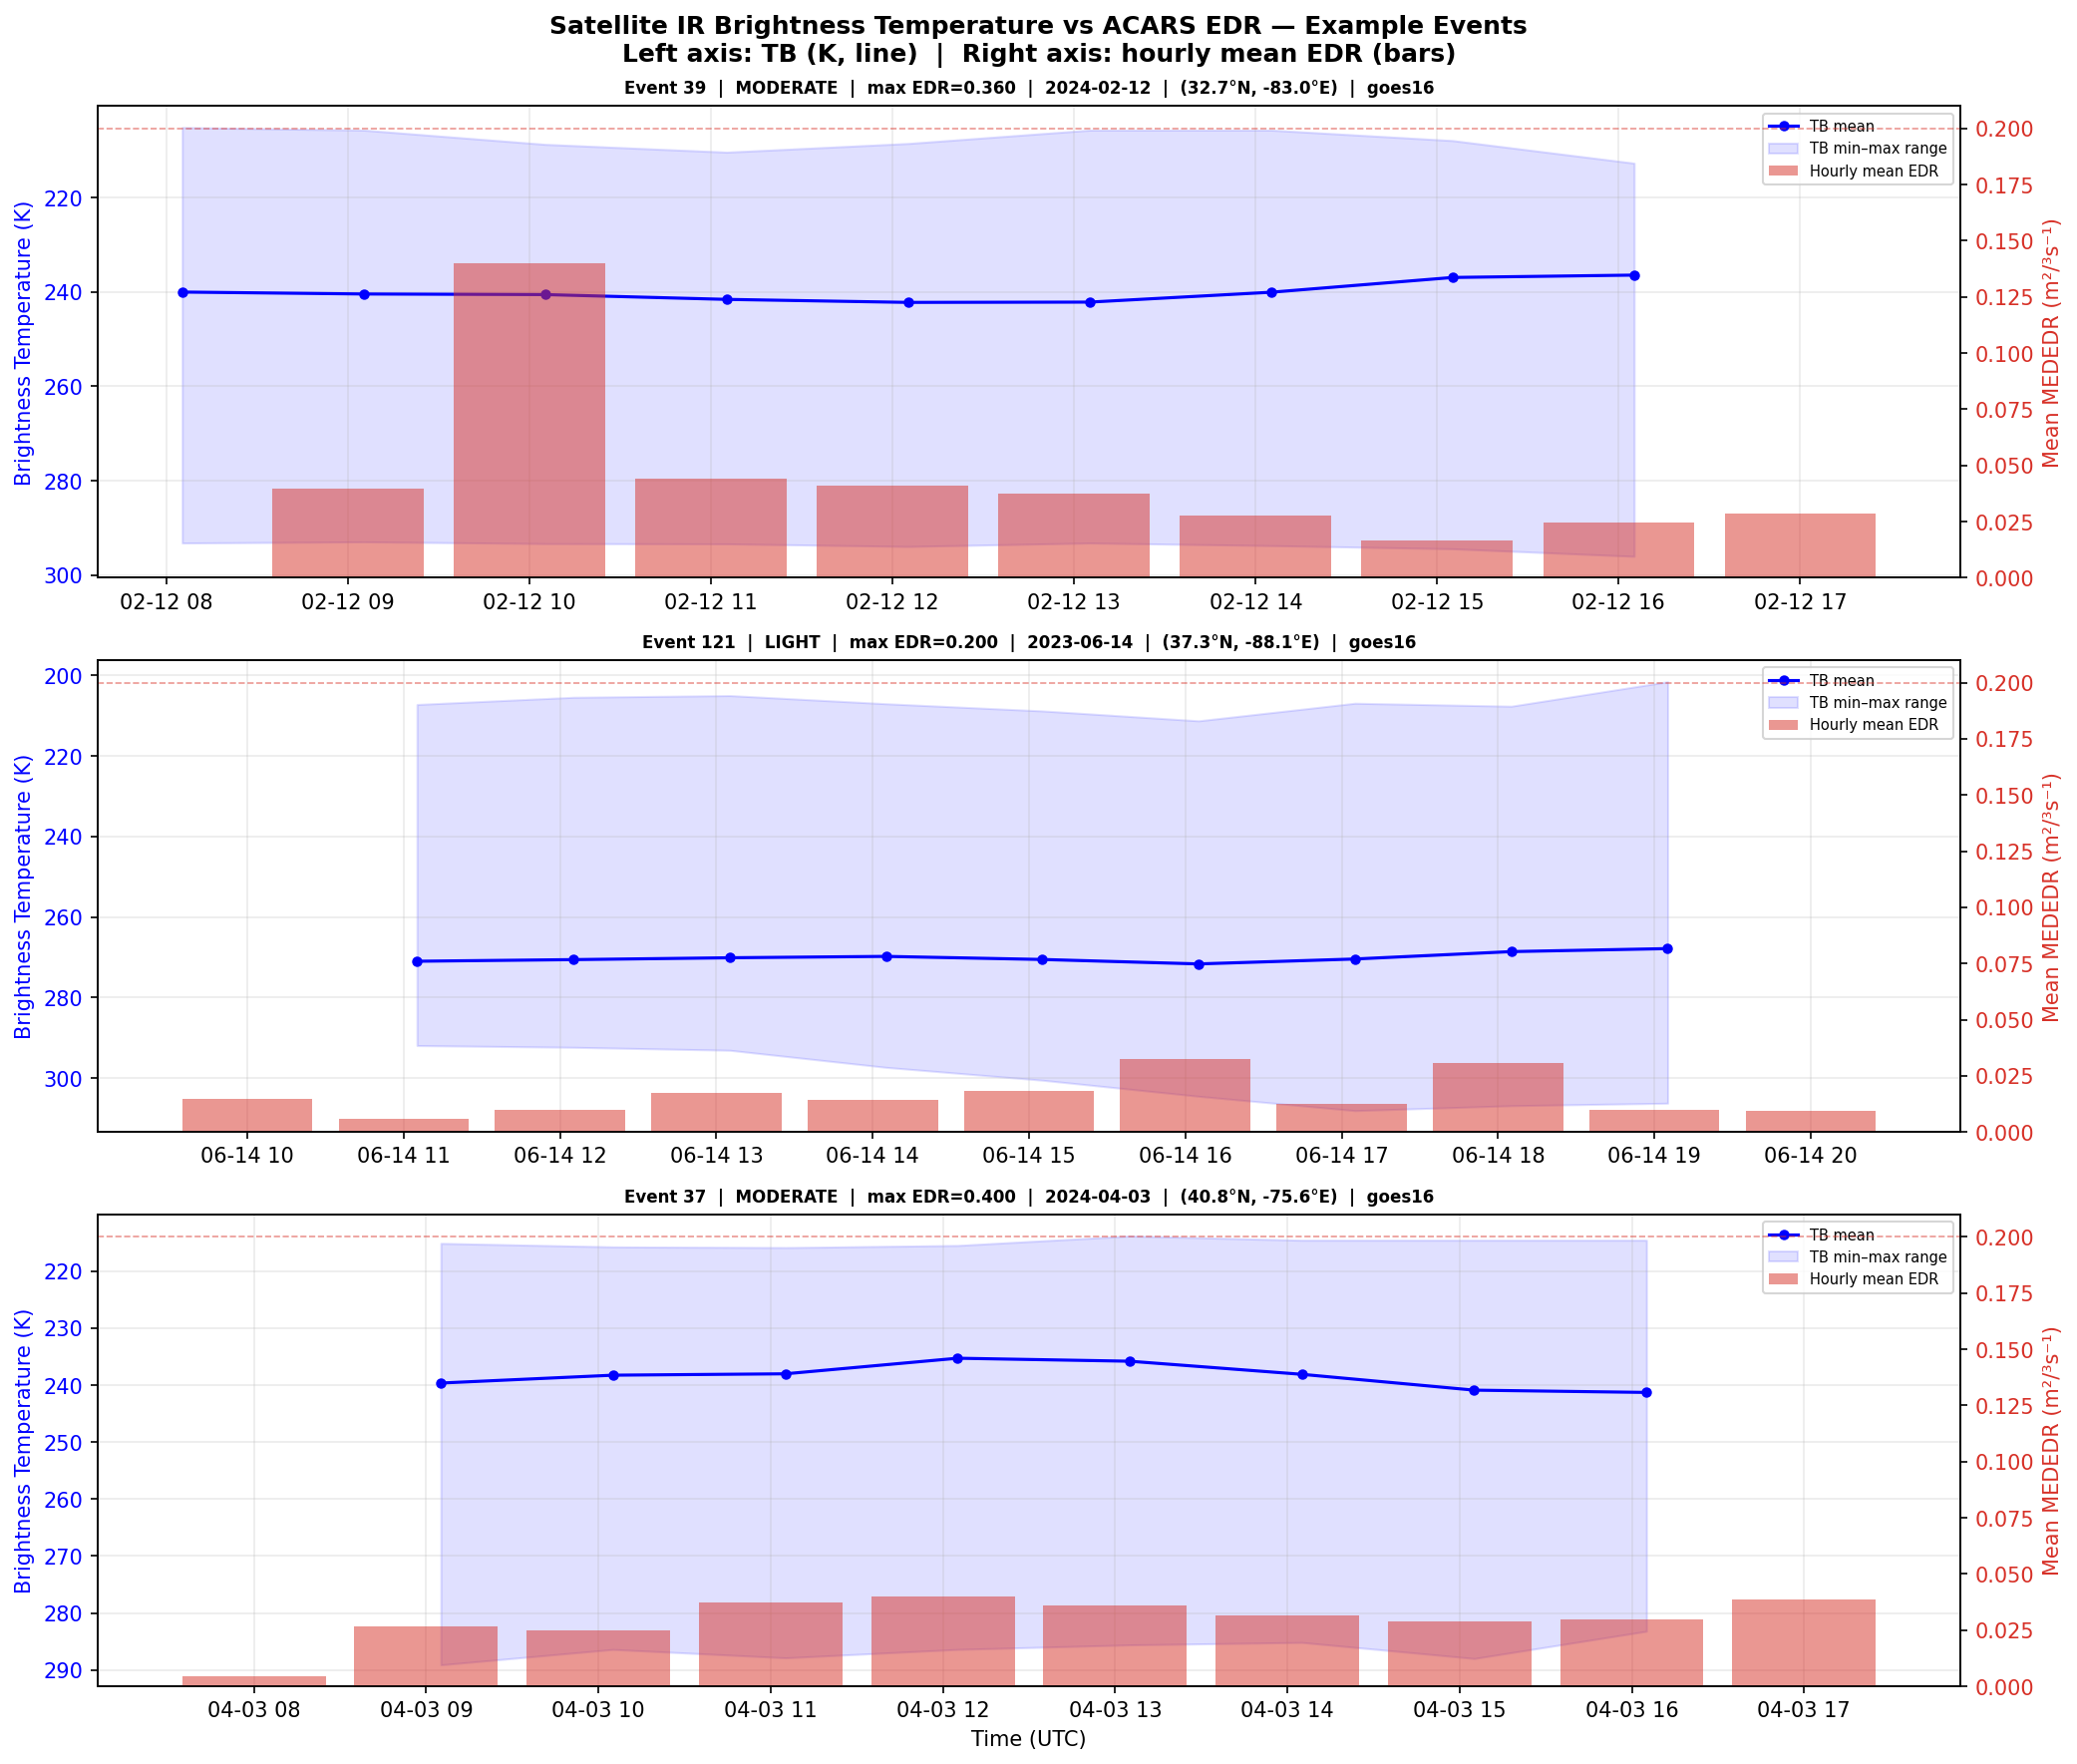
\includegraphics[width=0.88\linewidth]{opt5_timeseries_examples.png}
  \caption{Example events: satellite IR brightness temperature (line)
  vs.\ hourly mean EDR (bars). Cloud-top cooling tends to lead EDR peaks
  in convective cases.}
  \label{fig:sat-ts}
\end{figure}

\subsection{Principal component analysis}
\label{sec:eda-pca}
PCA of 16 ACARS event features shows PC1 (32.8\% variance) is an
EDR-intensity axis and PC2 (23.2\%) contrasts vertical extent with
geographic spread; severe events separate cleanly along $+$PC1, and the
first three PCs explain $>$80\% of variance (Fig.~\ref{fig:pca-acars}).
PCA of 29 ERA5 features yields a PC1 (41.4\%) that opposes vertical
velocity ($\omega$) against per-level wind speed---a shear/stability
axis---but events coloured by maximum EDR show only \emph{weak}
separation along it (Fig.~\ref{fig:pca-era5}). Bulk, spatially-averaged
atmospheric state is thus only weakly linearly separable by severity: the
events are not cleanly told apart by their mean diagnostics alone.
Geographic projection of the scores shows mild clustering, with the
highest-PC1 (most intense) events at higher latitudes
(Fig.~\ref{fig:pca-geo}).

\begin{figure}[H]
  \centering
  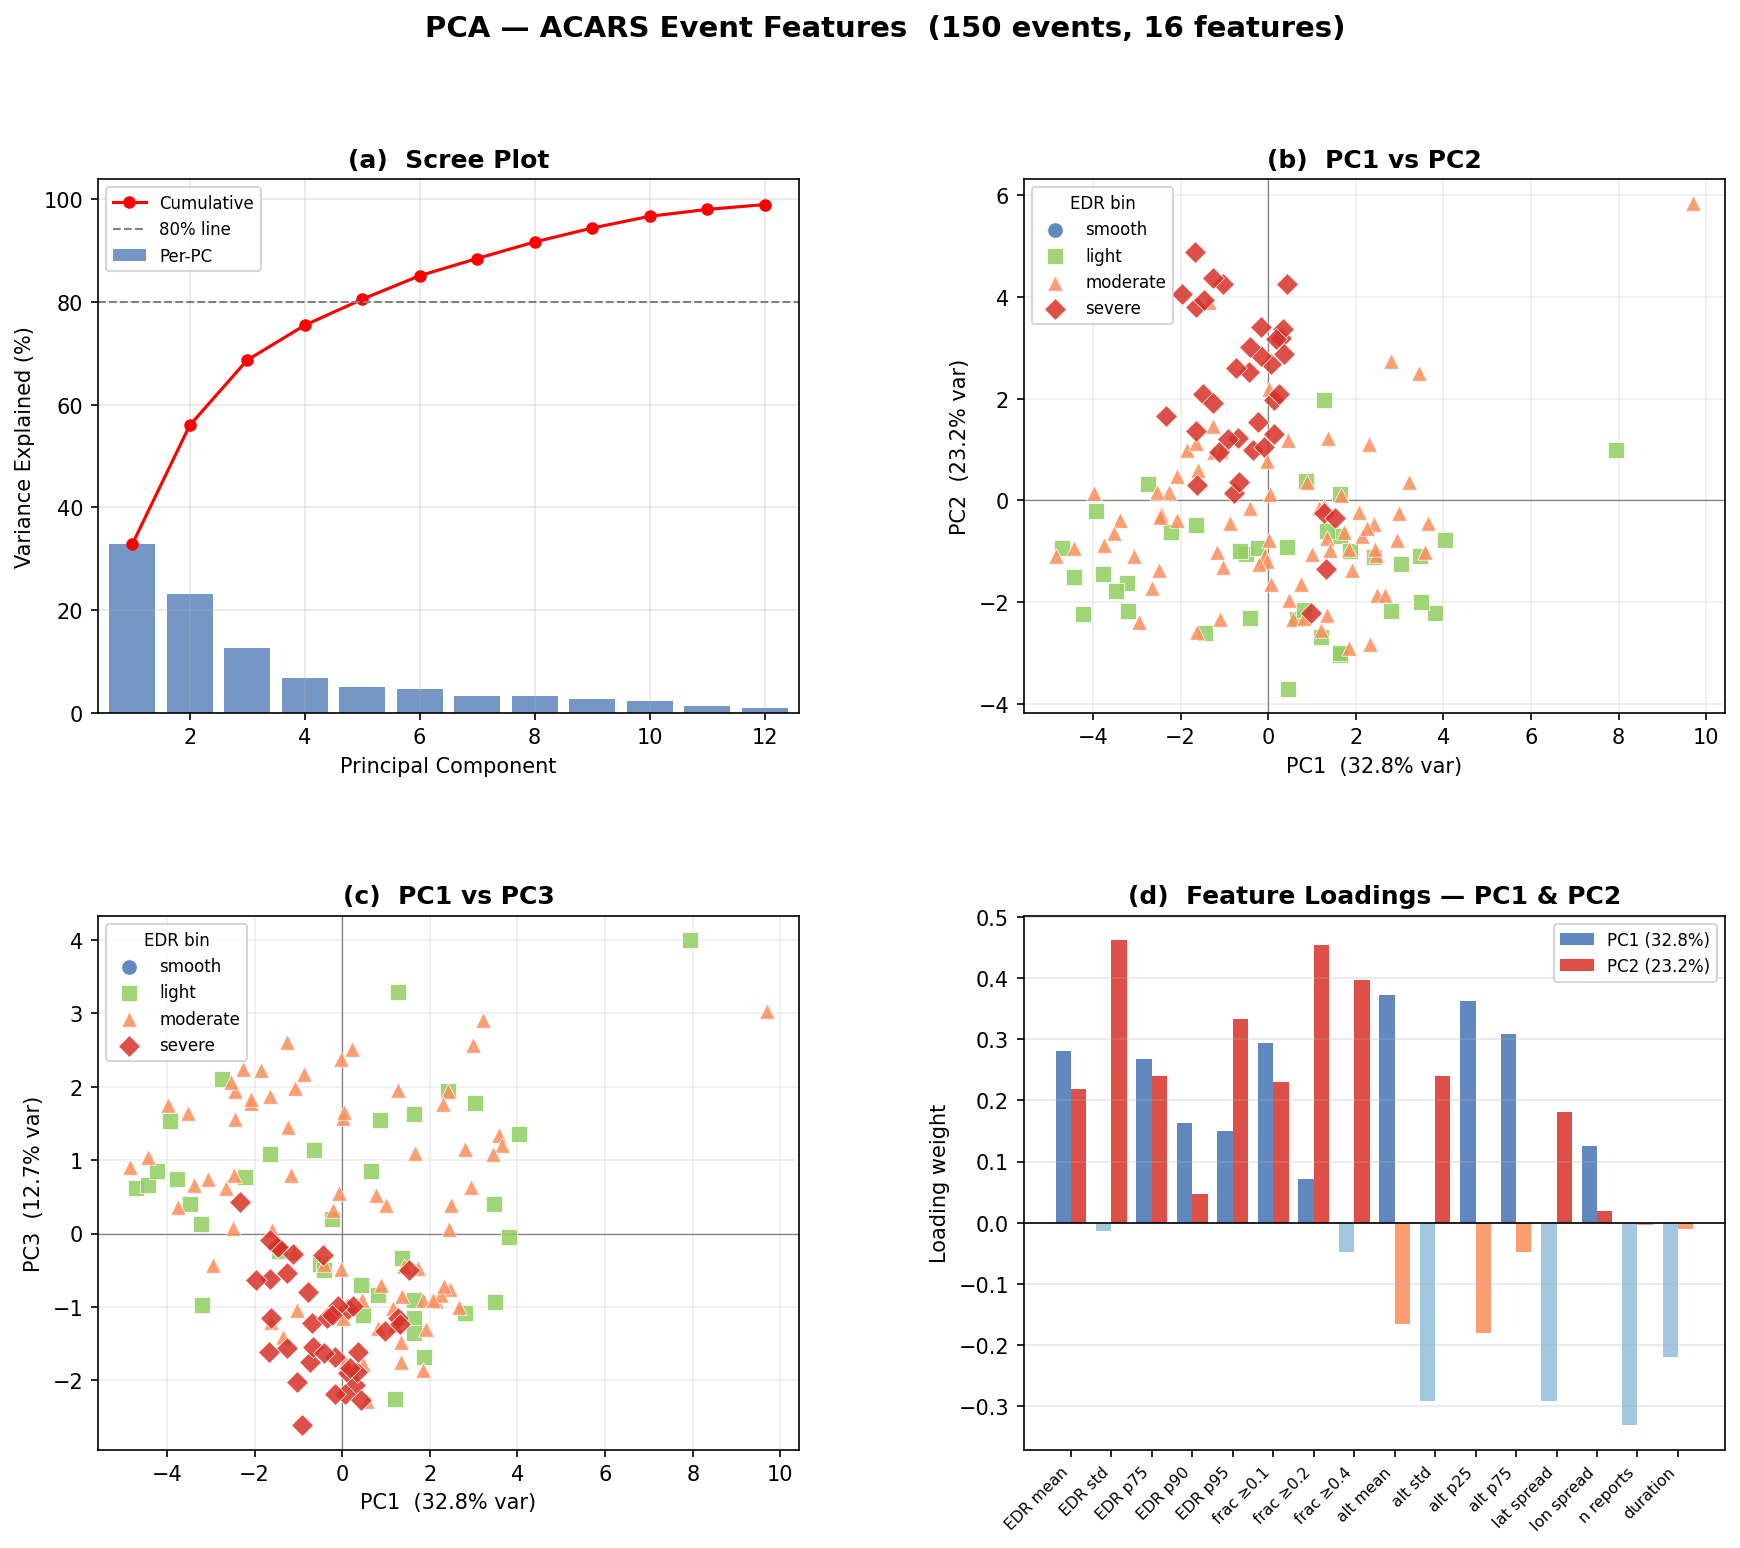
\includegraphics[width=0.88\linewidth]{pca_acars.png}
  \caption{PCA of ACARS event features (150 events, 16 features). PC1
  (32.8\%) is an EDR-intensity axis along which severe events separate;
  scree, PC1--PC2, PC1--PC3, and feature loadings shown.}
  \label{fig:pca-acars}
\end{figure}

\begin{figure}[H]
  \centering
  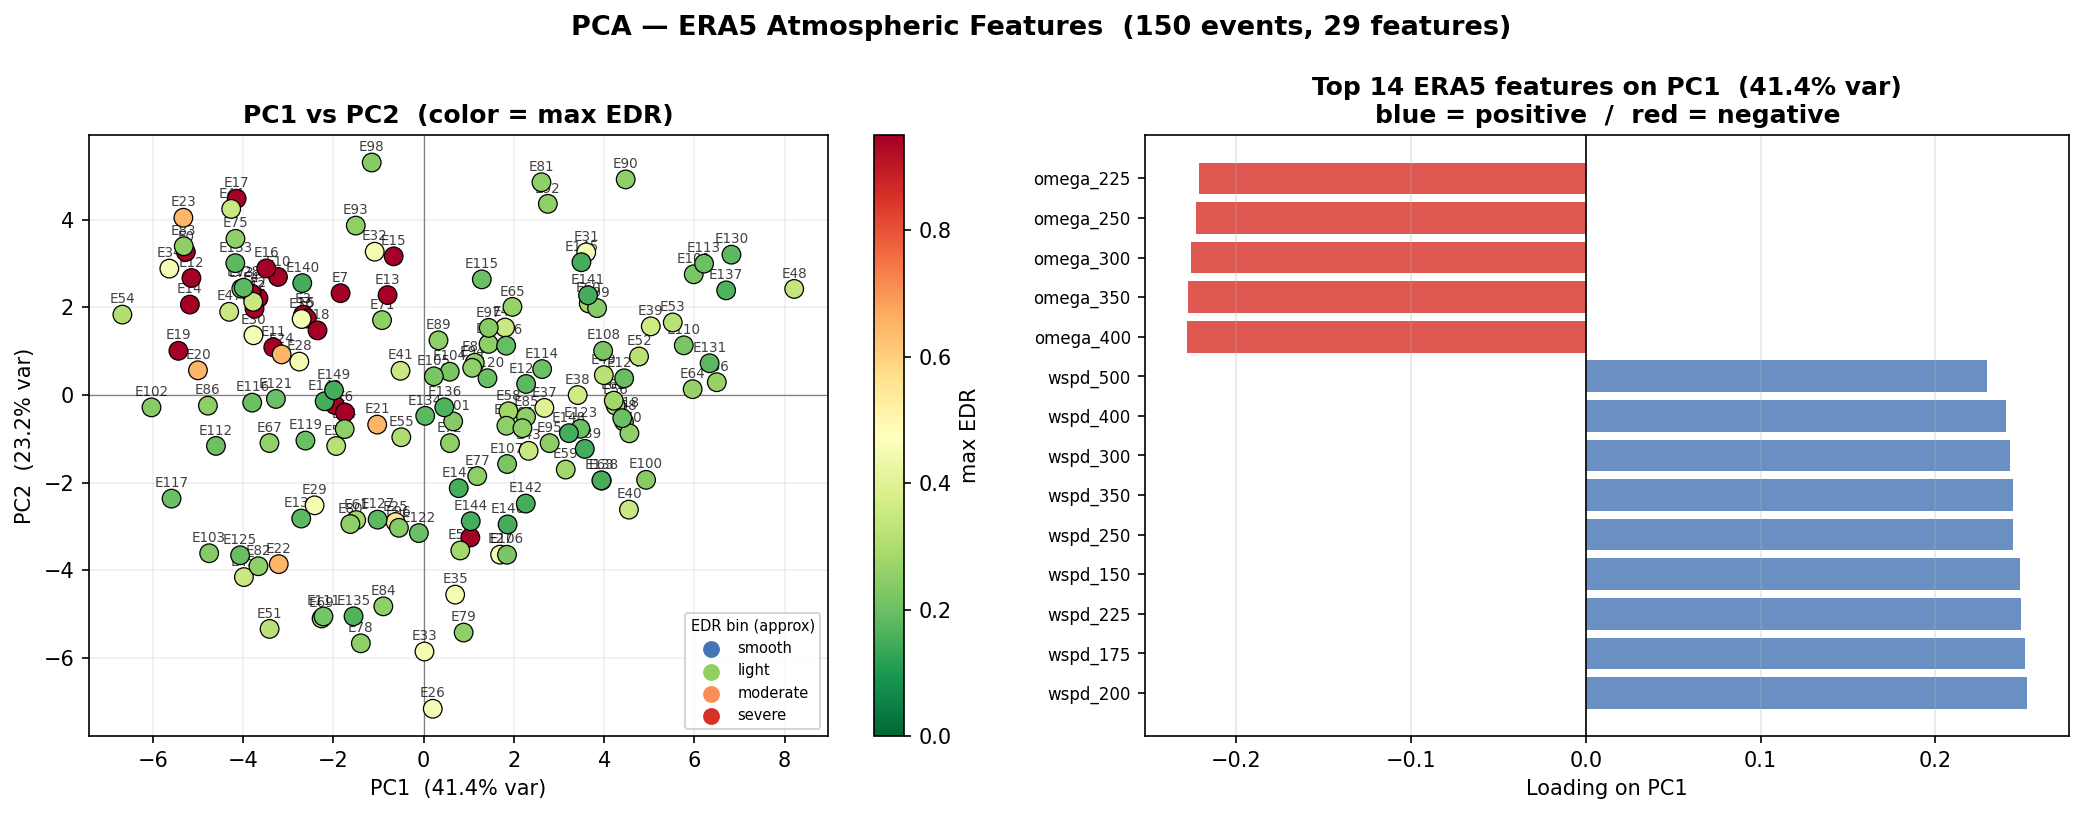
\includegraphics[width=0.88\linewidth]{pca_era5.png}
  \caption{PCA of ERA5 atmospheric features (29 features). PC1 (41.4\%)
  opposes vertical velocity against per-level wind speed (a
  shear/stability axis), but EDR severity is only weakly separated along
  it.}
  \label{fig:pca-era5}
\end{figure}

\begin{figure}[H]
  \centering
  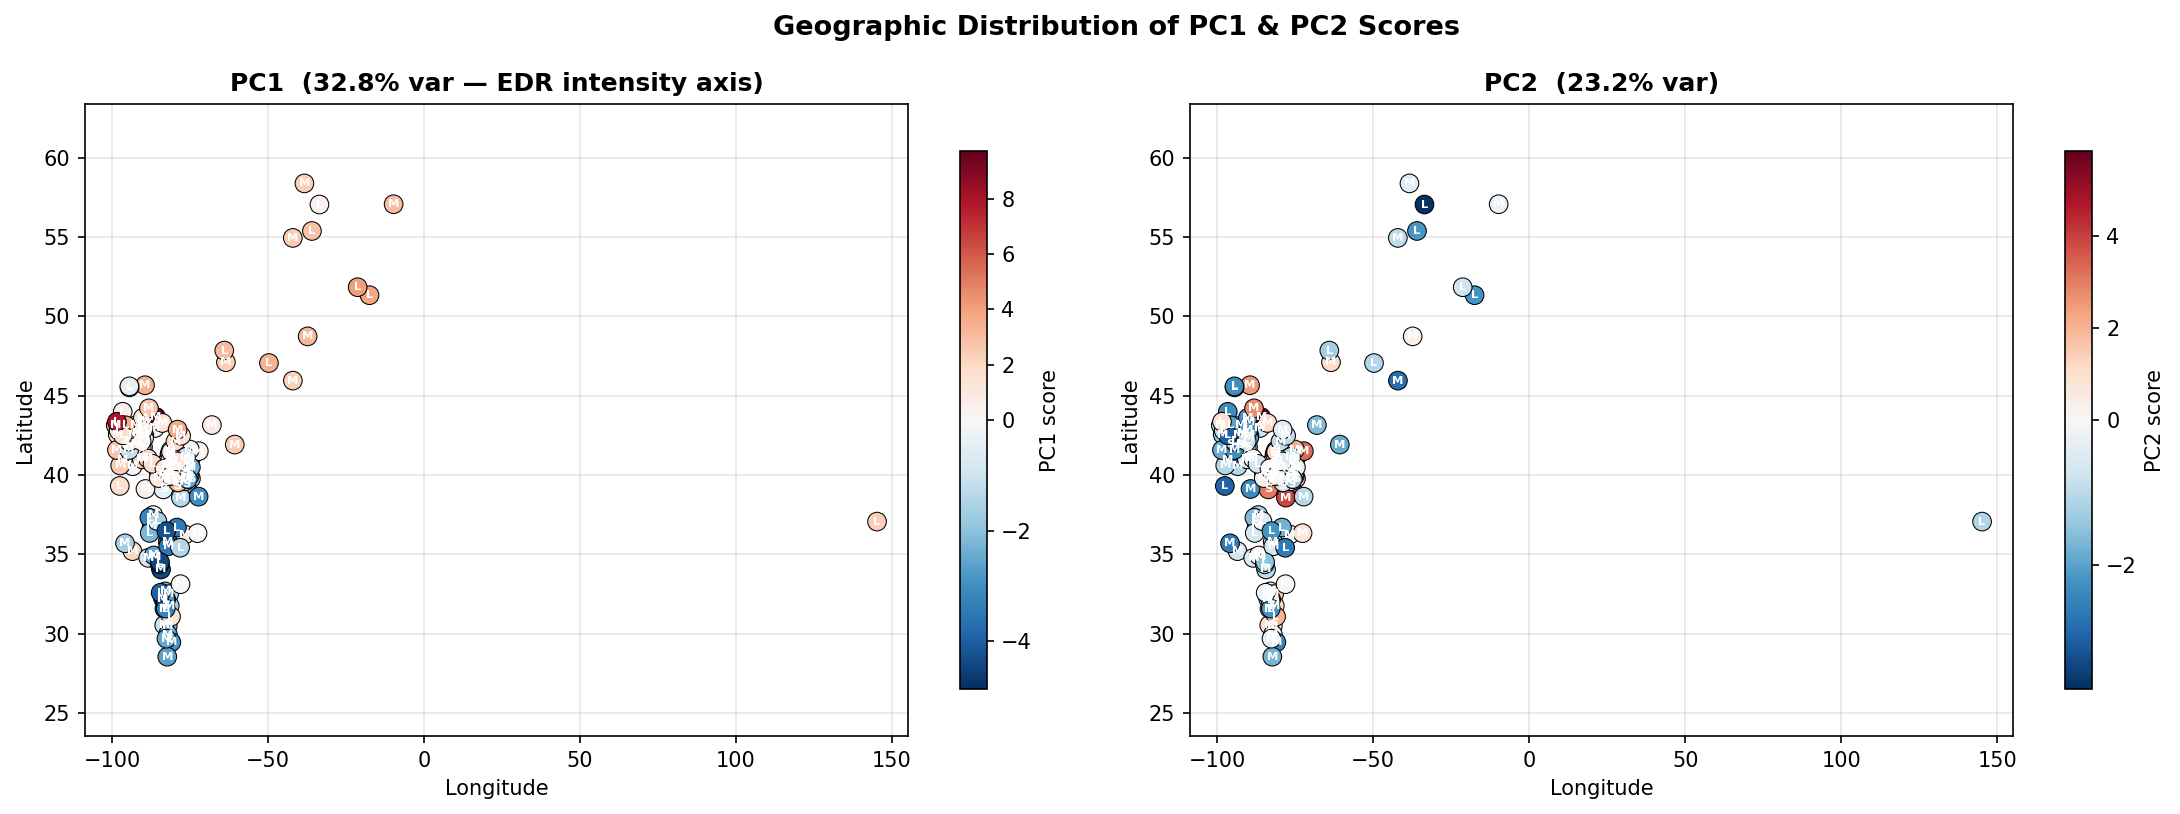
\includegraphics[width=0.88\linewidth]{pca_geo.png}
  \caption{Geographic distribution of PC1 (EDR-intensity) and PC2 scores
  by event centroid; most intense events cluster at higher latitudes.}
  \label{fig:pca-geo}
\end{figure}

% =====================================================================
\section{CNN Architecture}
\label{sec:arch}
The headline model is a physics-informed convolutional neural network
that keeps the operational GTG diagnostic ``vocabulary'' but replaces its
fixed weighted sum with a learned, spatial, non-linear mapping, trained
directly on continuous in-situ EDR. The complete architecture is shown in
Fig.~\ref{fig:model}. Its seven numbered components---\circnum{1}
physics-diagnostic inputs, \circnum{2} FiLM conditioning, \circnum{3} the
encoder, \circnum{4} the bottleneck and satellite fusion, \circnum{5} the
decoder, \circnum{6} the head and soft aggregation, and \circnum{7} the
physics-informed loss---are elaborated below, each with the reasoning
behind it. The pipeline is
ERA5\,+\,satellite\,+\,ACARS $\rightarrow$ diagnostics $\rightarrow$ CNN
$\rightarrow$ EDR field $\rightarrow$ soft-aggregated scalar EDR, with the
network holding $\sim$80k parameters.

\begin{figure}[H]
  \centering
  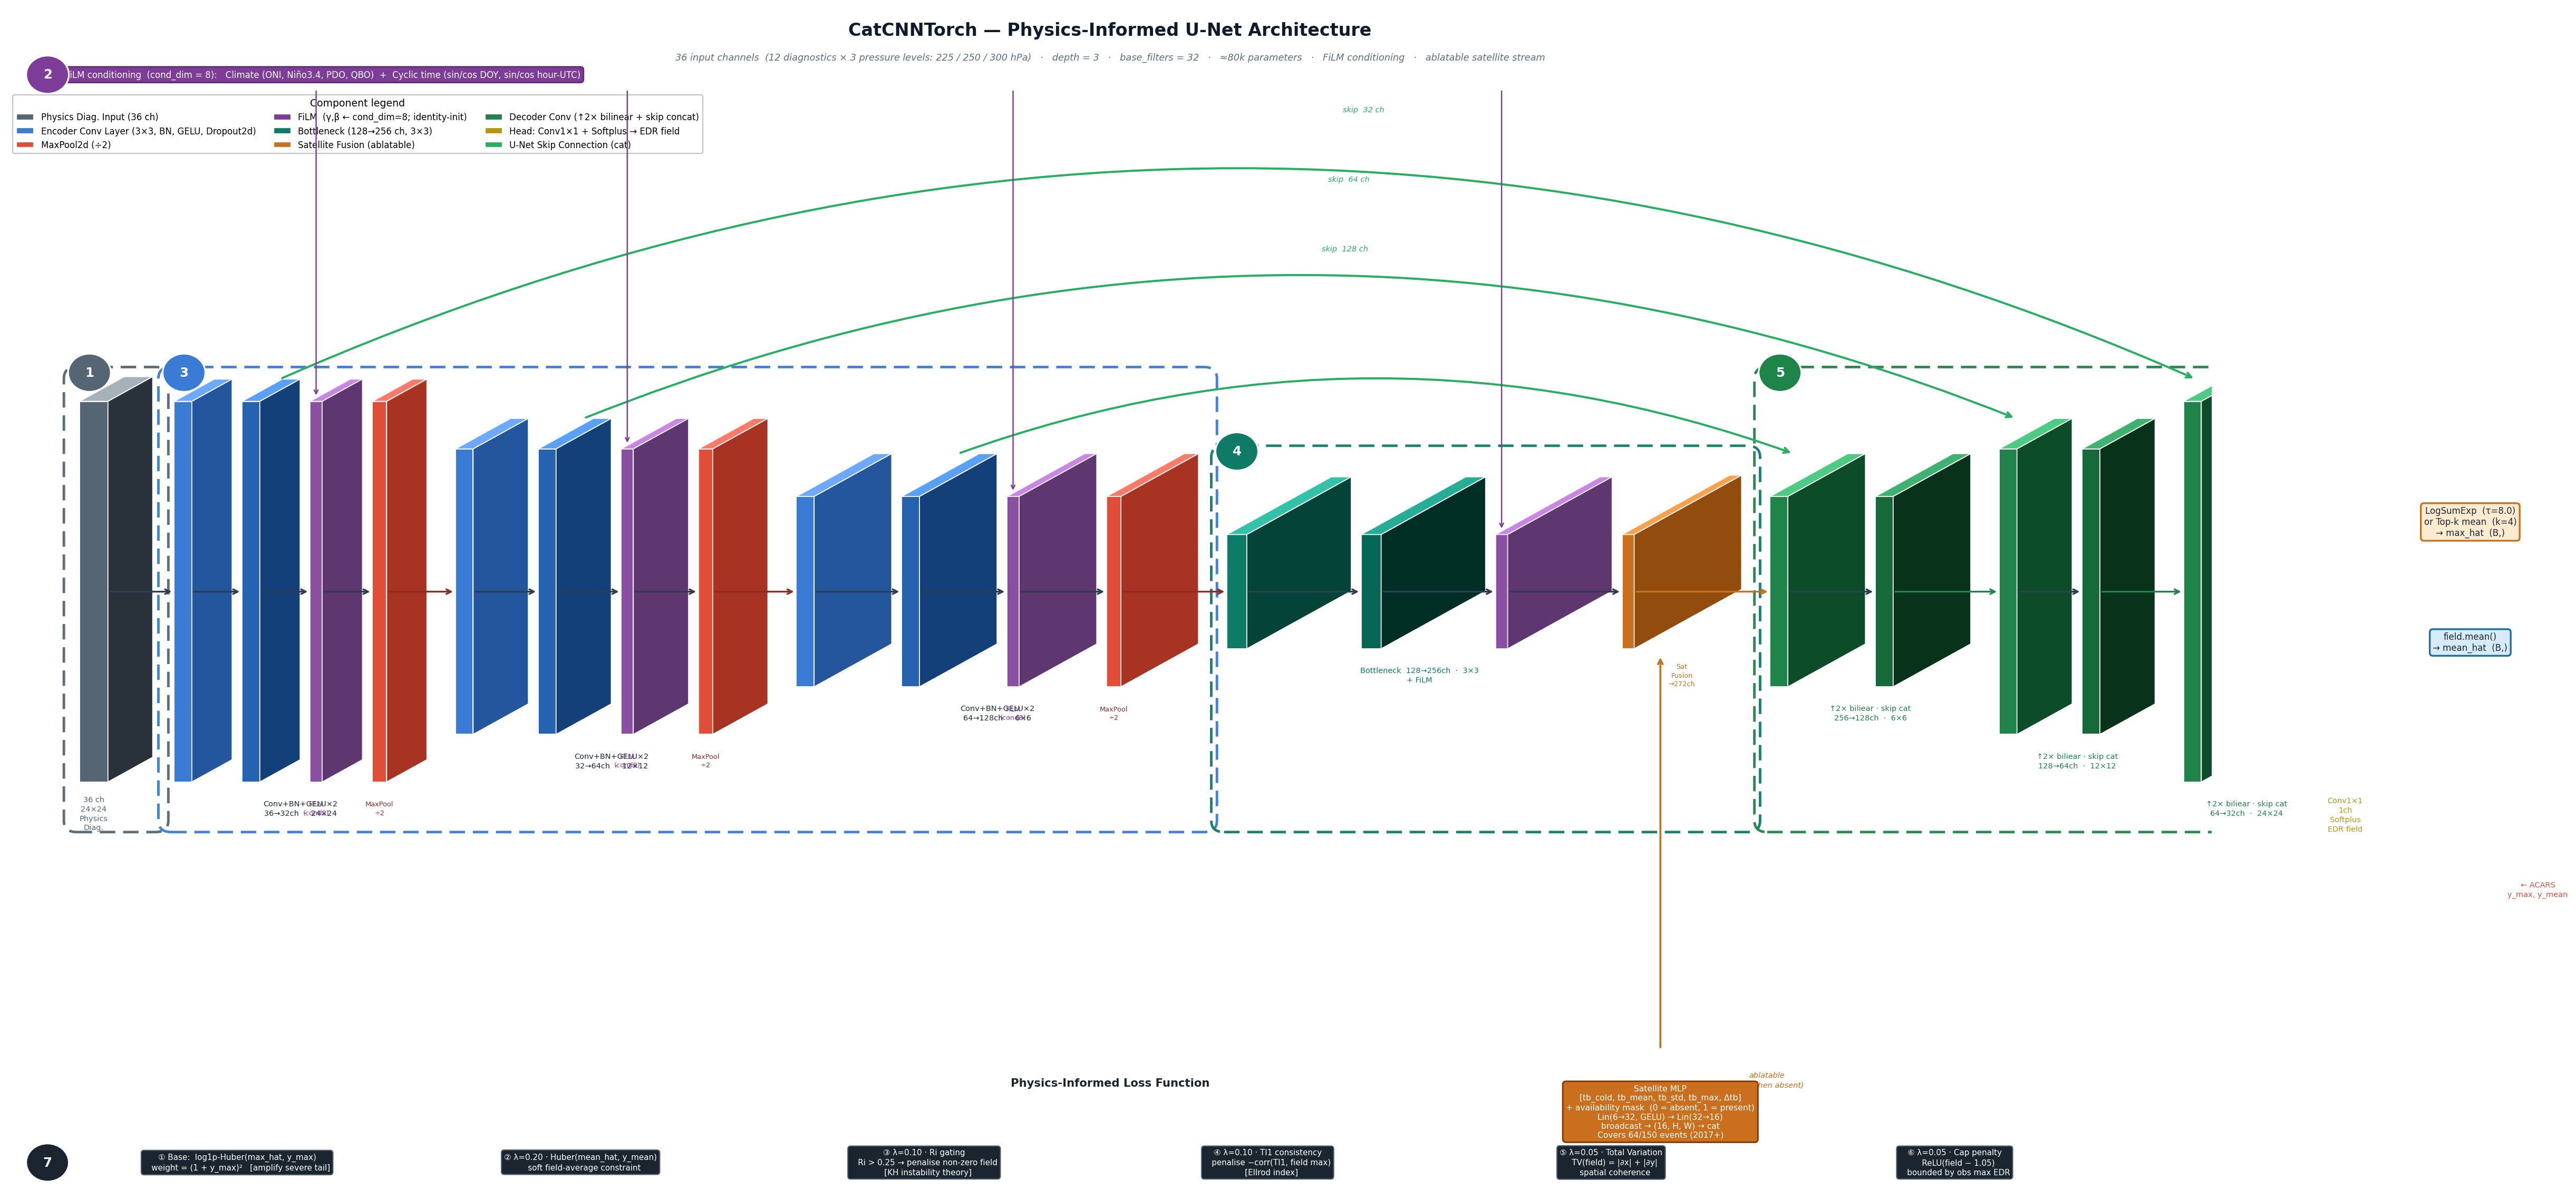
\includegraphics[width=\linewidth]{model.png}
  \caption{The physics-informed CatCNN. A two-stream encoder--decoder
  (U-Net) consumes 36 diagnostic channels (12 diagnostics $\times$ 3
  pressure levels), modulated by FiLM conditioning from climate and
  cyclic-time scalars and optionally fused with an ablatable satellite
  embedding at the bottleneck. The decoder reconstructs a dense EDR field
  through a softplus head; a differentiable soft aggregation reduces the
  field to the scalar EDR the labels provide. Numbered components
  \circnum{1}--\circnum{7} are elaborated in
  \S\ref{sec:arch-diag}--\S\ref{sec:arch-loss}.}
  \label{fig:model}
\end{figure}

\subsection{\circnum{1} Physics diagnostics as inputs}
\label{sec:arch-diag}
Rather than feeding raw $u,v,T$ fields, we hand the network 12 operational
CAT diagnostics computed per pressure level (Table~\ref{tab:diag}). The
reasoning is twofold. First, these diagnostics encode decades of CAT
physics---Kelvin--Helmholtz instability (Richardson number, vertical wind
shear), frontal dynamics (deformation, frontogenesis), and the Ellrod
turbulence indices---so the network starts from physically meaningful
quantities instead of having to rediscover them from wind components.
Second, the PCA of \S\ref{sec:eda-pca} showed that bulk atmospheric state
separates severity only weakly; presenting the non-linear diagnostic
combinations directly gives the network a far more separable input than
raw fields. Diagnostics are computed on the native ERA5 grid, bilinearly
resized to $24\times24$, log-compressed where heavy-tailed (VWS, DEF,
TI1, TI2, WSPD), and z-scored (statistics fit on the training split
only). With three jet-band levels (225/250/300\,hPa) this gives
$12\times3=\textbf{36 input channels}$. Constants: $g_0{=}9.80665$,
$R_d/c_p{=}0.286$, $P_0{=}1000$\,hPa; Ri is clipped to $[-5,50]$ to tame
the $1/\mathrm{VWS}^2$ tail.

\begin{table}[H]
\centering\small
\caption{Physics diagnostics computed per pressure level. $\theta$ is
potential temperature; $\zeta$ relative vorticity; $\mathbf{V}$
horizontal wind.}
\label{tab:diag}
\begin{tabular}{@{}lll@{}}
\toprule
Diagnostic & Formula & Role \\
\midrule
VWS & $\sqrt{(\partial_z u)^2+(\partial_z v)^2}$ & KH energy source\\
$N^2$ & $(g/\theta)\,\partial_z\theta$ & stratification \\
Ri & $N^2/\mathrm{VWS}^2$ & KH instability ($<0.25$)\\
DEF & $\sqrt{\mathrm{DST}^2+\mathrm{DSH}^2}$ & frontal tightening\\
DIV & $\partial_x u+\partial_y v$ & convergence \\
TI1 & $\mathrm{VWS}\cdot\mathrm{DEF}$ & Ellrod index 1\\
TI2 & $\mathrm{VWS}(\mathrm{DEF}-\mathrm{DIV})$ & Ellrod index 2\\
$\zeta$ & $\partial_x v-\partial_y u$ & rotation \\
FRONTO & Petterssen frontogenesis & jet/front CAT\\
WSPD & $\sqrt{u^2+v^2}$ & jet-core proxy\\
$\omega$ & (raw ERA5) & GW/convective forcing\\
VADV & $-\mathbf{V}\cdot\nabla\zeta$ & NVA predictor\\
\bottomrule
\end{tabular}
\end{table}

\subsection{\circnum{2} FiLM conditioning: climate and time/location}
\label{sec:arch-film}
Feature-wise Linear Modulation (FiLM) applies a per-channel affine
transform $\gamma\odot x+\beta$ to the feature maps, where $\gamma$ and
$\beta$ are generated by a small network from a conditioning vector. We
apply FiLM after every encoder block and at the bottleneck, and
\emph{identity-initialise} it ($\gamma{=}1,\beta{=}0$) so conditioning
begins as a no-op and the network only leans on it if it helps. FiLM is
the right mechanism precisely because the exploratory analysis showed
these signals are \emph{weak modulators, not primary drivers}: the
seasonal--trend decomposition (\S\ref{sec:eda-seasonal}) attributes
$\sim$90\% of daily variance to synoptic weather, so season and climate
should adjust, not dominate, a physics-driven prediction.

\paragraph{Why include climate indices (ONI, Ni\~no3.4, PDO, QBO).} The
EEMD of \S\ref{sec:eda-eemd} found genuine multi-year ($\sim$4\,yr) and
decadal ($\sim$8\,yr) oscillatory energy in turbulence intensity, which
motivated testing the named climate oscillations. That test
(\S\ref{sec:eda-climate}) returned \emph{no} statistically significant
teleconnection under phase-randomised surrogates. This null result is
exactly why we neither discard the indices nor hard-code a weight for
them: we supply ONI, Ni\~no3.4, PDO, and QBO as FiLM conditioning and let
the identity-initialised network learn whatever small weight the data
support---if there is no usable signal, FiLM simply stays near identity.

\paragraph{Why include cyclic time and location.} The climatology
(\S\ref{sec:eda-seasonal}) and the regional analysis
(\S\ref{sec:eda-regional}) establish that encounter rate depends strongly
on season and on geography. Figure~\ref{fig:single-region} isolates a
single region (E North America) to make the point concrete: even within
one region the month axis carries a clear winter-heavy structure. We
therefore encode date and time as cyclic features ($\sin/\cos$ of
day-of-year and hour, keeping December and January adjacent) and feed
them through FiLM; location enters through the geography of the event box
and the spatial grid itself. Because the diurnal signal is weak, the hour
term is kept deliberately minimal.

\begin{figure}[H]
  \centering
  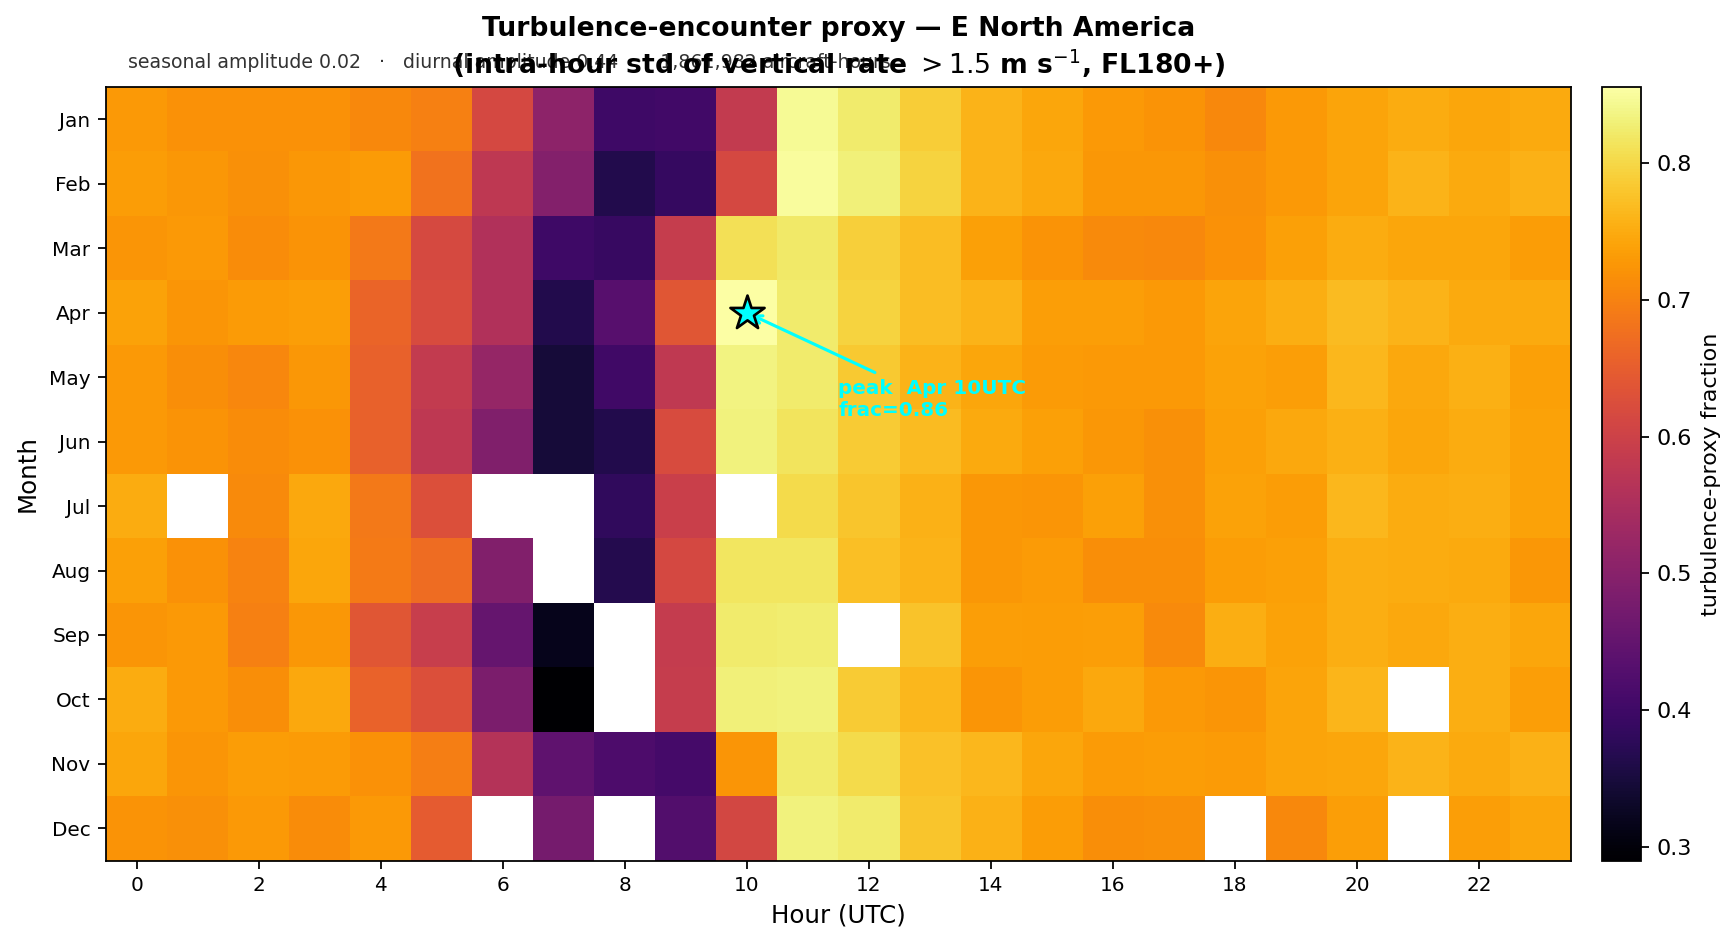
\includegraphics[width=0.82\linewidth]{single_region.png}
  \caption{Turbulence-encounter proxy for a single region (E North
  America), month $\times$ hour. Even within one region the seasonal
  (month) structure is pronounced---turbulence is far more likely in
  winter---justifying cyclic-time conditioning. Contrast the full
  15-region grid of Fig.~\ref{fig:regional}.}
  \label{fig:single-region}
\end{figure}

\subsection{\circnum{3}\,\circnum{5} Encoder--decoder and \circnum{6} head with soft aggregation}
\label{sec:arch-unet}
The backbone is a two-stream encoder--decoder (U-Net-like) with
``same'' padding throughout (default depth~3:
$24\!\to\!12\!\to\!6\!\to\!3$; base width 32 doubling per block; each
block Conv\,$\to$\,Norm\,$\to$\,Act\,$\to$\,Dropout\,$\to$\,Conv\,$\to$\,Norm\,$\to$\,Act
with a residual $1\times1$ shortcut). A U-Net suits CAT because the
phenomenon is mesoscale: the encoder captures the broad jet/frontal
context while \textbf{skip connections} carry fine spatial detail to the
decoder, so the reconstructed field can resolve the compact patches in
which turbulence actually occurs. The \circnum{6} head is a $1\times1$
convolution (a shared per-pixel MLP) followed by a \textbf{softplus},
which enforces $\mathrm{EDR}\geq 0$ without saturating the heavy upper
tail the way a sigmoid would.

Because the labels are scalar (no gridded EDR exists), a differentiable
\textbf{soft aggregation} reduces the predicted field to a scalar that can
be supervised: log-sum-exp with a searchable temperature $\tau$ (default
8.0) approximates the field maximum for sparse fields while staying
smooth and differentiable, with a top-$k$ mean as an alternative. The
spatial mean is aggregated separately to an auxiliary mean-EDR target.
This is the mechanism that lets a field-predicting network train on
scalar supervision.

\subsection{\circnum{4} Satellite stream (ablatable)}
\label{sec:arch-sat}
A small satellite MLP embeds the five brightness-temperature statistics
plus a present/absent mask and fuses the embedding at the bottleneck. It
is \textbf{ablatable}: when satellite data are absent the input is zeros
with the mask set accordingly, so the network learns to ignore the stream
rather than hallucinate from missing data. This design is forced by the
data: \S\ref{sec:eda-sat} showed satellite covers only 64 of 150 events
(all post-2017) and is blind to severe clear-sky jet CAT. The stream must
therefore be structurally optional, and toggling it on and off is exactly
the structural test for \textbf{RQ2}---whether cloud-top information adds
skill over reanalysis alone.

\subsection{\circnum{7} Physics-informed loss}
\label{sec:arch-loss}
We train on $\log\mathrm{1p}(\mathrm{EDR})$ (inverting with the inverse
transform) to stabilise the heavy tail. The base term is a
magnitude-weighted Huber ($\delta{=}0.1$) on the log-aggregated maximum
versus the log label, with weight $1+w_{\mathrm{mag}}y$ emphasising the
rare severe tail, plus an auxiliary Huber on the mean
($w_{\mathrm{aux}}{=}0.2$). Five physics-penalty terms, each with a
searched weight $\lambda_i$, shape the \emph{field} given only scalar
supervision:
\begin{enumerate}
  \item \textbf{Non-negativity} backstop, $\mathrm{relu}(-\hat{y})^2$.
  \item \textbf{Shear--stratification gating}: penalise high predicted
  EDR where the flow is dynamically stable (Ri\,$\gg$\,1) \emph{and}
  low-shear, where no turbulent energy is available---this writes
  Kelvin--Helmholtz theory directly into the loss.
  \item \textbf{Ellrod-TI consistency}: penalise negative rank-correlation
  between the predicted field and the TI1 field, so the network may refine
  but not invert the physics.
  \item \textbf{Total variation}: a small penalty enforcing the coherent
  patch structure of real CAT.
  \item \textbf{Climatological bound}: penalise predictions exceeding the
  observed maximum (0.95).
\end{enumerate}
Together these turn unconstrained field reconstruction into a
physically-plausible one even though only a single scalar per event is
ever observed.

\subsection{Design-space search}
\label{sec:arch-design}
Rather than hand-tuning the many choices above, we select them by
held-out skill with an automated design-space search
(Fig.~\ref{fig:design}). A TPE sampler proposes a configuration spanning
architecture (depth, width, kernel, norm, activation, pooling, dropout),
the FiLM and satellite toggles, the head, the aggregation type and its
$\tau/k$, the optimiser, and every loss weight $\lambda$; each candidate
is trained under 4-fold \textbf{event-grouped} cross-validation (no event
split across folds, so no leakage) on an 80-epoch budget; a median pruner
kills underperformers early; and the sampler updates its posterior over
40 trials. The search objective is
$\text{log-RMSE}+(1-\text{AUPRC}@0.20)$, which balances tail-accurate
regression against rare-event (severe) discrimination. Every architectural
decision is thus chosen by validation skill, not by hand.

\begin{figure}[H]
  \centering
  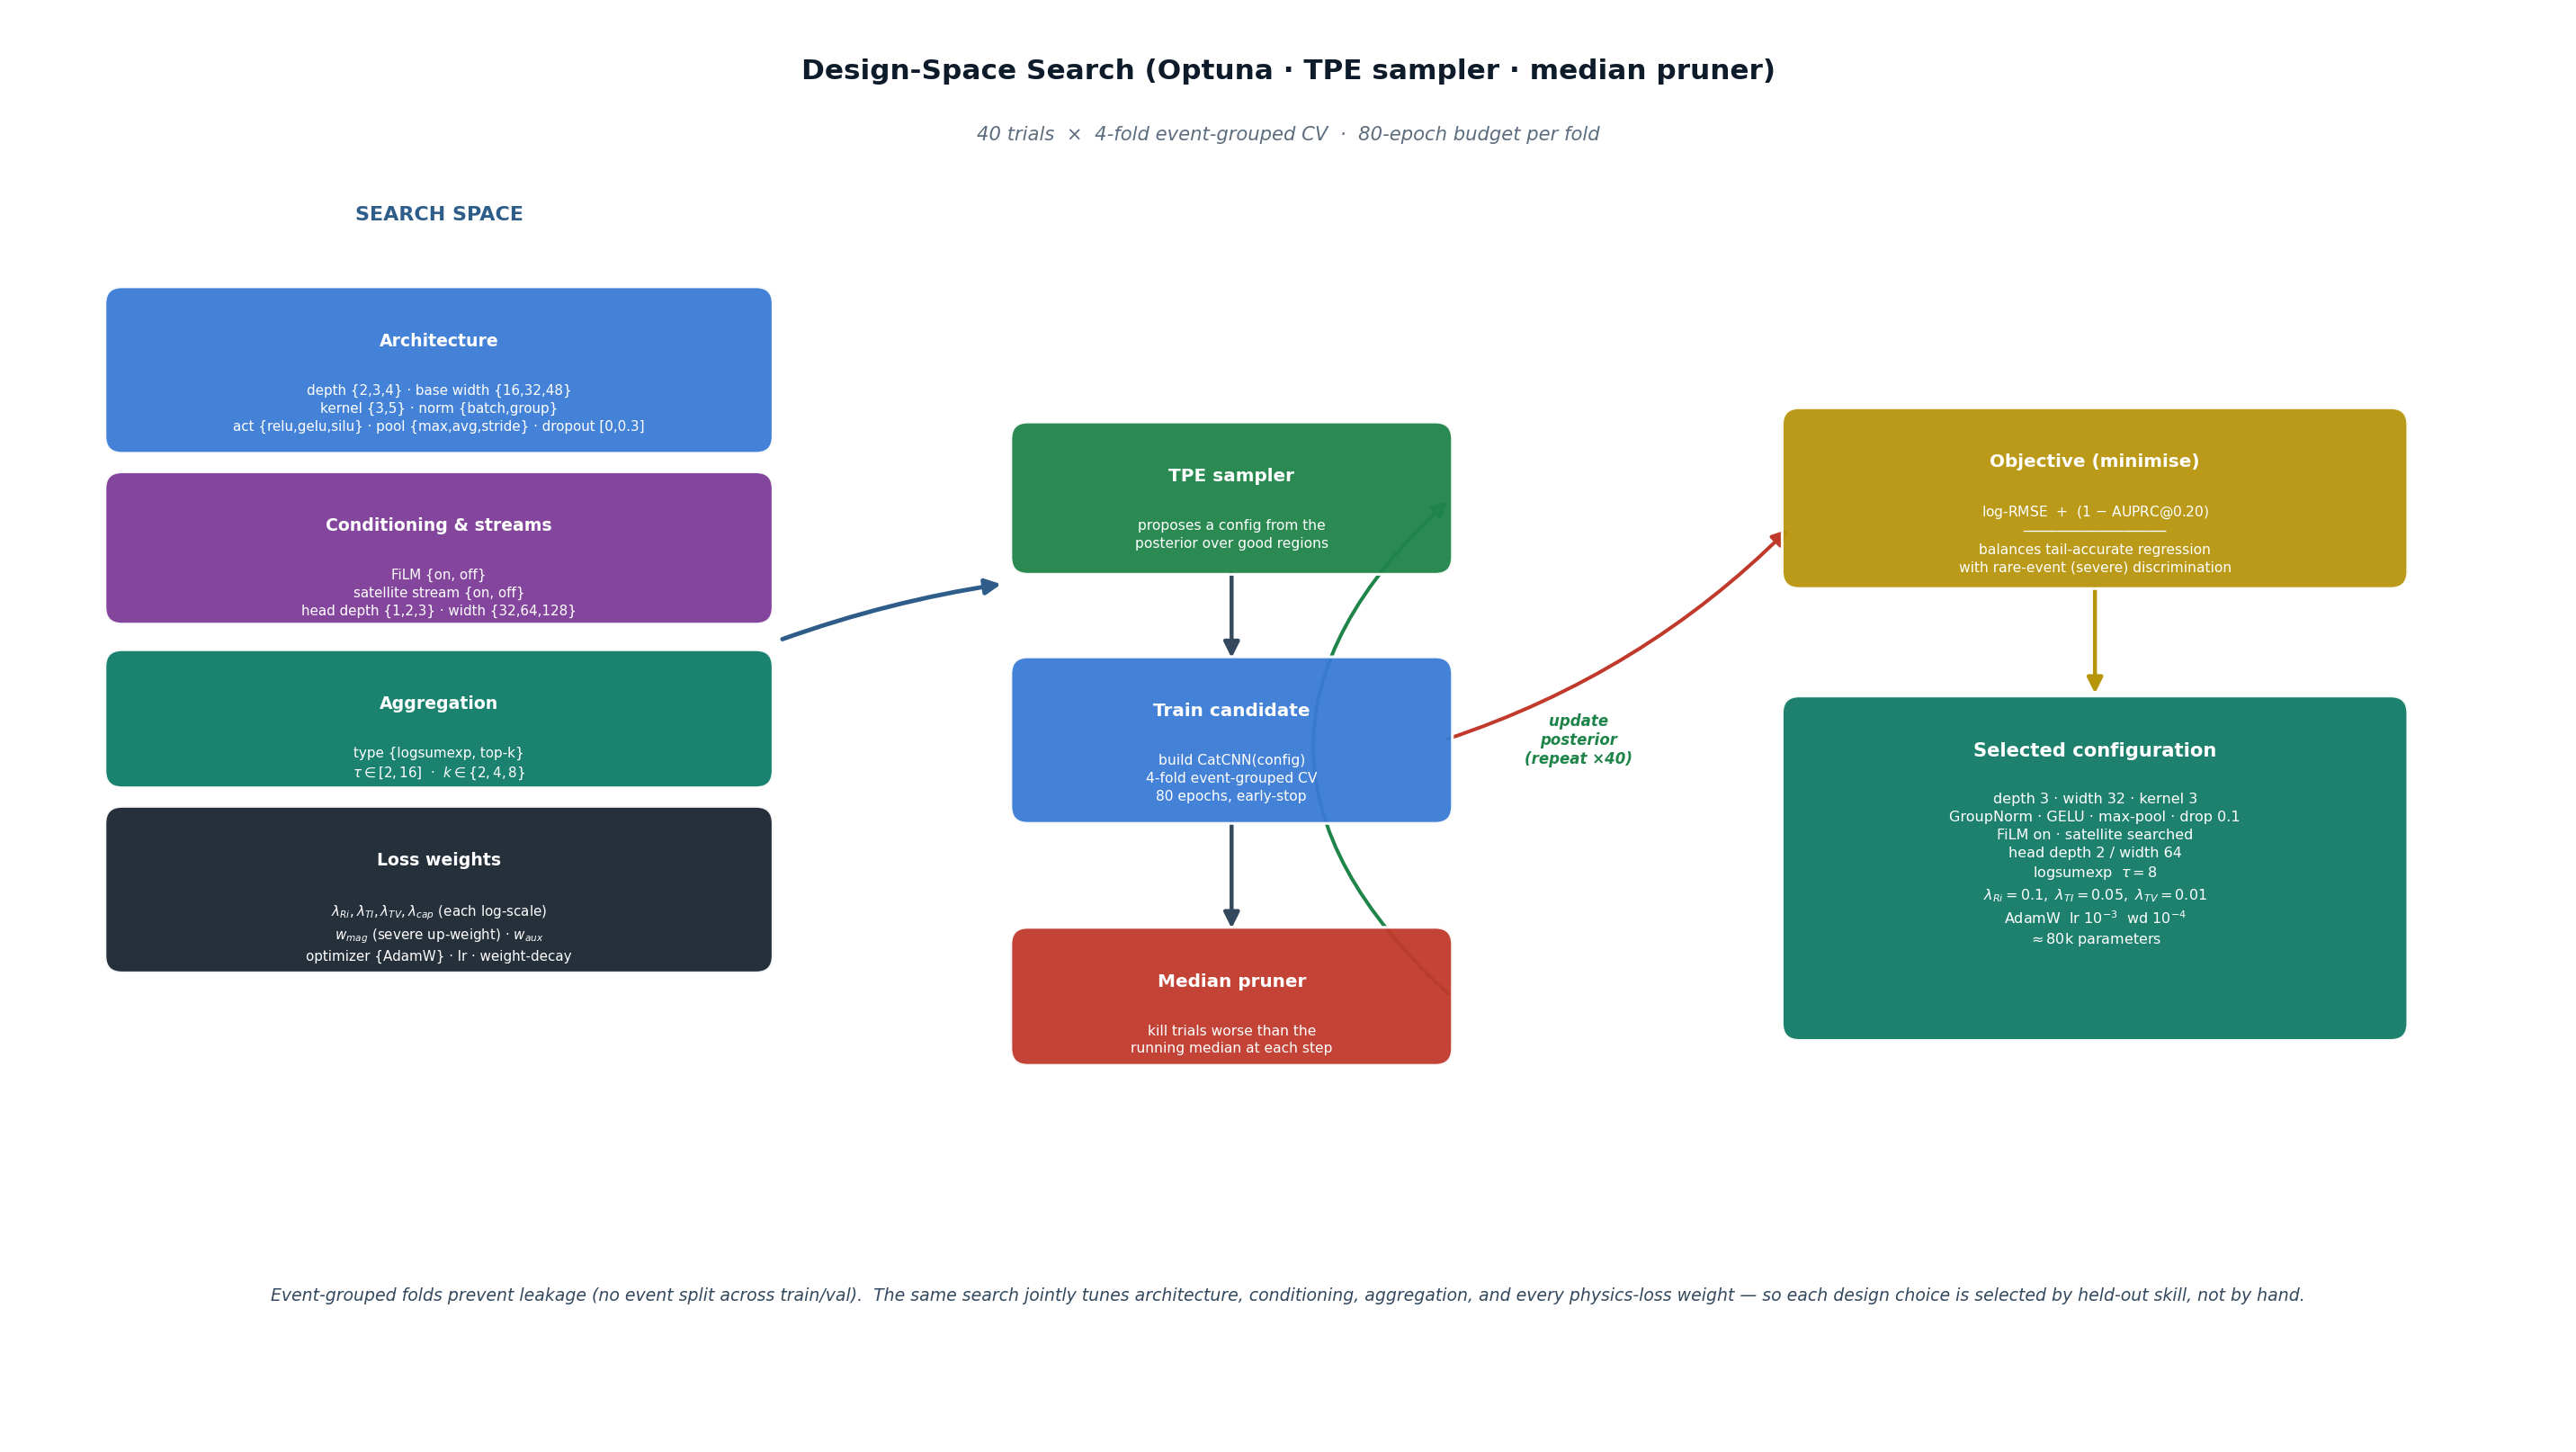
\includegraphics[width=0.95\linewidth]{design_space.png}
  \caption{The design-space search. The search space (left) is sampled by
  a TPE sampler that trains each candidate under event-grouped 4-fold CV,
  prunes weak trials, and updates its posterior; the selected
  configuration (right) is the one minimising
  log-RMSE\,$+\,(1-\text{AUPRC}@0.20)$.}
  \label{fig:design}
\end{figure}

\subsection{Training protocol}
\label{sec:arch-train}
The final model is trained with a \textbf{temporal hold-out} (most-recent
20\% of events) plus event-grouped, severity-stratified $k$-fold CV.
Optimisation uses AdamW (lr~$10^{-3}$, weight decay~$10^{-4}$, batch~16),
up to 200 epochs with patience~30 and gradient clipping at 5; augmentation
is restricted to axis flips (wind vectors are not rotation-invariant).

\subsection{Open design question: direct vs.\ residual}
\label{sec:residual}
The architecture supports both direct prediction (built) and a
\emph{physics-residual} formulation
$\mathrm{EDR}=\text{surrogate}(\text{Ellrod/GTG})+\text{ML(residual)}$. We
retain this as an explicit planned A/B rather than baking it in: residual
learning can ease training on small data and gives a clean ``does ML beat
physics'' narrative, while direct prediction avoids surrogate bias.

% =====================================================================
\section{Results}
\label{sec:results}
This section reports the physics-informed CatCNN only; the head-to-head
comparison against baselines follows in \S\ref{sec:eval}. All figures here
use the leakage-safe protocol of \S\ref{sec:arch-train}: the model is
evaluated by 5-fold \textbf{event-grouped out-of-fold (OOF)}
cross-validation, so every prediction is made on an event the model never
trained on.

\subsection{Out-of-fold accuracy}
\label{sec:res-acc}
Pooled across the five held-out folds (127 events), the CatCNN attains
\textbf{Pearson $r=0.878$} and \textbf{RMSE $0.153$~\edrunit}
(MAE~$0.119$), with strong moderate-exceedance discrimination
(\textbf{AUROC~$0.872$, AUPRC~$0.867$} at the $0.20$ threshold;
Table~\ref{tab:catcnn}, Fig.~\ref{fig:predobs}a). Because every point is a
genuine held-out prediction, this is a far more honest figure than an
in-sample fit: an OOF correlation near $0.88$ confirms that the
reanalysis-derived diagnostics carry strong, generalisable EDR signal.
Per-fold scores (Table~\ref{tab:catcnn}) range from $r=0.59$ to $0.88$;
the spread reflects how few and how heterogeneous 150 events are, and the
pooled OOF value is the headline.

\paragraph{A note on the temporal hold-out.} In addition to the OOF folds
we set aside the 23 most-recent events as a final hold-out. These happen
to be \emph{all light} (maximum EDR $0.15$--$0.18$, standard deviation
$0.014$), so a correlation coefficient on them is meaningless---there is
essentially no target variance to correlate against---even though the RMSE
($0.18$) is in line with the OOF value. We therefore report the OOF
cross-validation as the evaluation of record and note the hold-out only
for completeness.

\begin{table}[H]
\centering\small
\caption{CatCNN out-of-fold cross-validation. Top: per-fold scores;
bottom: pooled OOF over all 127 held-out events (the headline).}
\label{tab:catcnn}
\begin{tabular}{@{}lrrrrr@{}}
\toprule
Fold & RMSE & log-RMSE & Pearson & AUPRC & AUROC \\
\midrule
0 & 0.180 & 0.119 & 0.764 & 0.818 & 0.822 \\
1 & 0.168 & 0.110 & 0.857 & 0.894 & 0.867 \\
2 & 0.175 & 0.114 & 0.877 & 0.802 & 0.800 \\
3 & 0.208 & 0.132 & 0.603 & 0.845 & 0.826 \\
4 & 0.202 & 0.134 & 0.592 & 0.732 & 0.748 \\
\midrule
\textbf{Pooled OOF} & \textbf{0.153} & --- & \textbf{0.878} & \textbf{0.867} & \textbf{0.872} \\
\bottomrule
\end{tabular}
\end{table}

\begin{figure}[H]
  \centering
  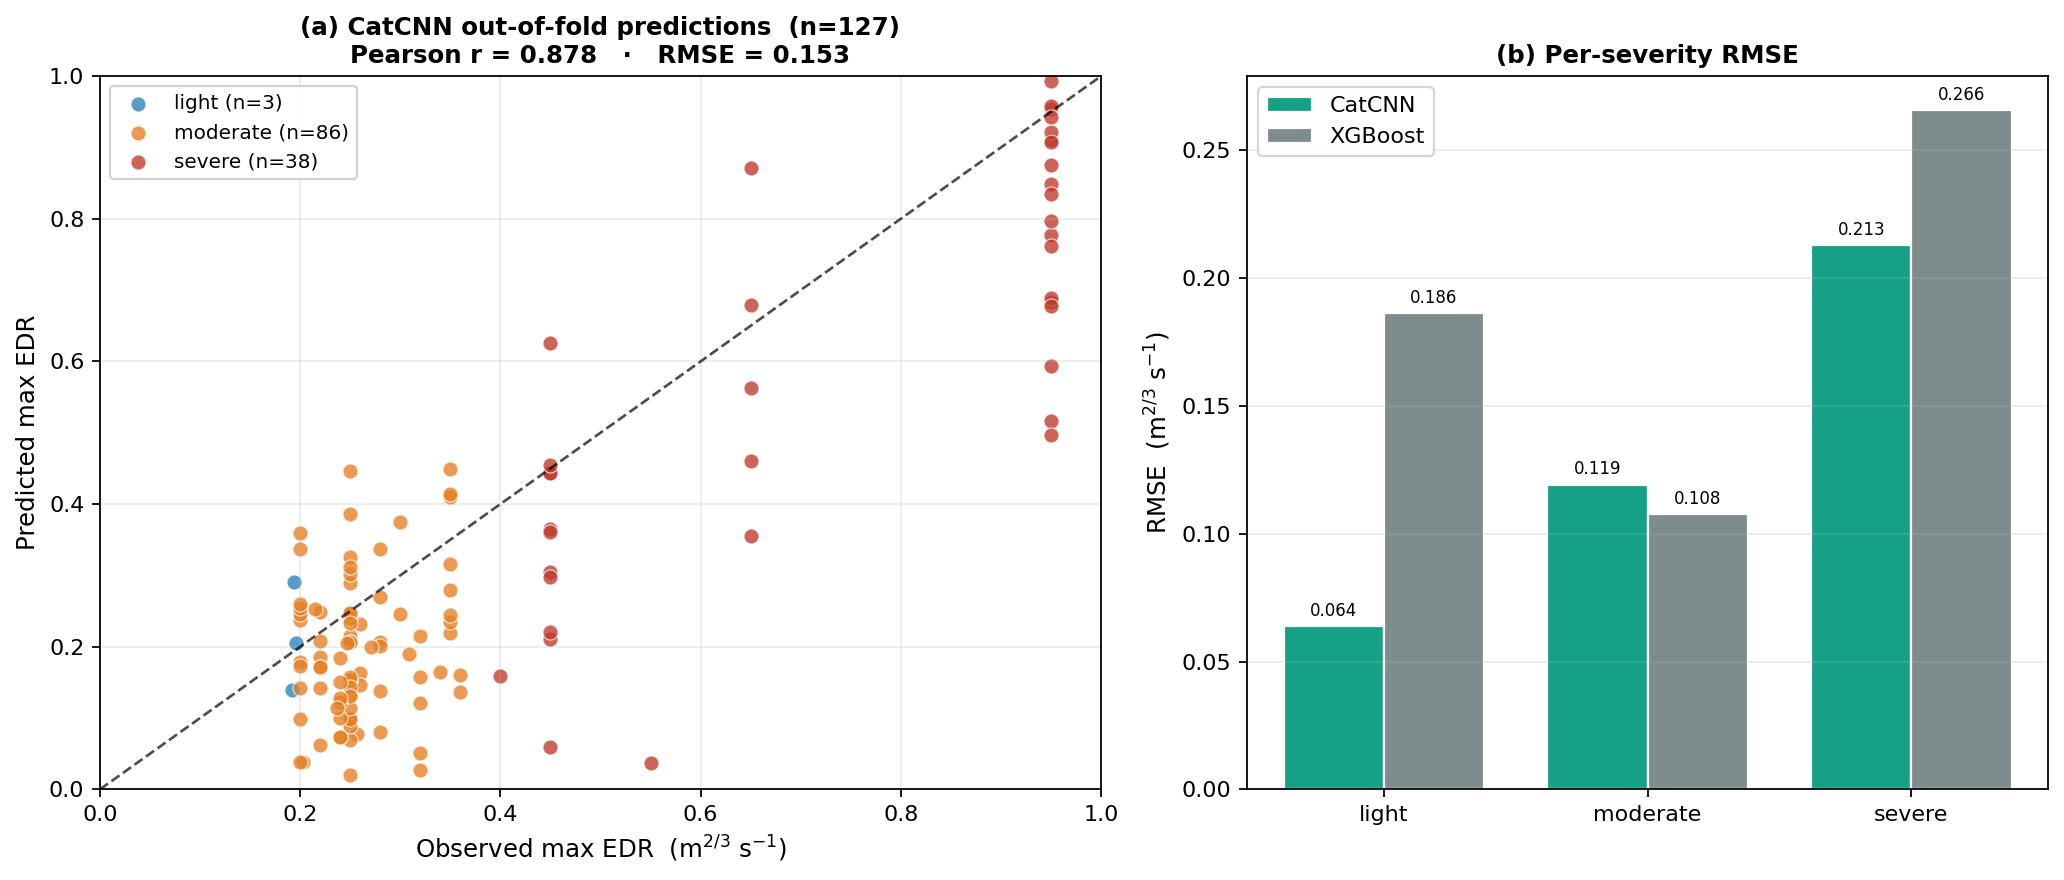
\includegraphics[width=0.95\linewidth]{cnn_pred_vs_obs.png}
  \caption{CatCNN out-of-fold predictions. (a)~Predicted vs.\ observed
  maximum EDR over the 127 held-out events, coloured by severity bin (1:1
  dashed); pooled $r=0.878$, RMSE $0.153$. (b)~RMSE by severity bin for
  CatCNN vs.\ XGBoost---the CNN is more accurate in every bin, most
  decisively in the safety-critical severe tail.}
  \label{fig:predobs}
\end{figure}

\subsection{Behaviour across the severity range}
\label{sec:res-bins}
The error remains tail-concentrated: severe-bin OOF RMSE ($0.213$) is
roughly double the moderate-bin value ($0.119$), and the light bin shows
near-zero correlation, the classic heavy-tail pattern in which the model
is sharpest in the middle of the distribution. Crucially, the
$\log\mathrm{1p}$ target and magnitude-weighted loss of
\S\ref{sec:arch-loss} keep the severe-tail Pearson high ($r=0.80$ within
the severe bin), so the model still ranks the most dangerous events
correctly even where absolute error is largest---and it beats XGBoost in
every bin (Fig.~\ref{fig:predobs}b).

% =====================================================================
\section{Model Evaluation}
\label{sec:eval}
To judge whether the CatCNN's skill is meaningful we compare it against
three references chosen to span the methodological spectrum---a plain
neural network, a pure machine-learning regressor, and the operational
physics system. Each isolates a different question.

\subsection{Reference CNN (does the physics machinery help?)}
\label{sec:eval-cnn}
A from-scratch convolutional network provides a dependency-free, vanilla
reference. It takes 18 \emph{raw} ERA5 channels (6 variables $\times$ 3
levels) on a $24\times24$ grid through
Conv($18\!\to\!16$)\,$\to$\,ReLU\,$\to$\,MaxPool\,$\to$\,Conv($16\!\to\!32$)\,$\to$\,ReLU\,$\to$\,MaxPool\,$\to$\,GlobalAvgPool\,$\to$\,FC\,$\to$\,sigmoid
($\sim$8.3k parameters), regressing normalised maximum EDR under MSE. The
gap between this reference and the CatCNN measures what the physics
machinery---diagnostic inputs, FiLM conditioning, soft aggregation, and
the physics-penalty loss---actually buys over a plain CNN on raw fields.
Evaluated under a simpler 80/20 split (not the grouped OOF protocol), it
reaches $r=0.885$ overall but only $r=0.736$ on its held-out validation
events---so on genuinely unseen data the plain CNN already falls below the
CatCNN's $0.878$ out-of-fold correlation.

\subsection{XGBoost (does spatial structure help?)}
\label{sec:eval-xgb}
The gradient-boosted baseline regresses the log maximum EDR on
\textbf{spatially pooled} features: the per-channel mean, max, and
standard deviation of all 36 diagnostics, concatenated with the climate,
cyclic-time, and satellite scalars ($\sim$121 features), with deliberately
modest hyperparameters (400 trees, depth~4, lr~0.03, subsample/colsample
0.8) evaluated out-of-fold. XGBoost collapses each event's fields to
summary statistics, so it captures \emph{how strong} the diagnostics are
but discards \emph{where} and \emph{in what arrangement}. \textbf{The
CatCNN-vs-XGBoost gap therefore isolates the value of spatial structure
itself}: if the CNN cannot beat pooled features, the convolutional
machinery is not earning its keep. The PCA of \S\ref{sec:eda-pca}, where
bulk state separates severity only weakly, predicts that pooled features
should plateau and that spatial context should help---XGBoost makes that
hypothesis testable, and supplies an interpretable feature-importance
ranking to cross-check the network against the physics. It is also the
substrate for the residual-hybrid question of \S\ref{sec:residual}.

\subsection{NOAA GTG surrogate (does learning beat the operational sum?)}
\label{sec:eval-gtg}
The physics surrogate emulates operational GTG/GTCC: each diagnostic is
log-normal-calibrated to an EDR estimate and combined through a weight
vector, here optimised for ROC-AUC at the moderate threshold via
differential evolution, with the fitted weights compared to GTG
climatological weights as a sanity check. This is the system the CatCNN
must beat: it shares GTG's diagnostic vocabulary, so the comparison
asks directly whether a learned, spatial, non-linear combination
outperforms the fixed weighted sum operational forecasting relies on.
\emph{(Specified; not yet run---its row in Table~\ref{tab:compare}
remains open.)}

\subsection{Metrics and head-to-head comparison}
\label{sec:eval-metrics}
We report RMSE, MAE, and Pearson correlation on EDR, and AUROC and AUPRC
for moderate exceedance ($\mathrm{EDR}\geq 0.20$). CatCNN and XGBoost are
compared on the \emph{same} event-grouped out-of-fold basis
(Table~\ref{tab:compare}, Fig.~\ref{fig:compare}). \textbf{The
physics-informed CatCNN wins on every metric}: it cuts RMSE by 14\%
($0.153$ vs.\ $0.179$) and, more tellingly, lifts the Pearson correlation
from $0.705$ to $0.878$ and the AUPRC from $0.752$ to $0.867$. Since
XGBoost sees the \emph{same} diagnostics as pooled mean/max/std statistics
and differs only in discarding spatial layout, this gap is direct evidence
that \textbf{spatial structure carries real, learnable skill}---exactly
what the weak severity separation in the ERA5 PCA (\S\ref{sec:eda-pca})
predicted. The plain reference CNN, evaluated on its held-out validation
split, sits between the two ($r=0.736$): adding the physics machinery to a
CNN, and giving it diagnostics rather than raw fields, moves held-out
correlation from $0.736$ to $0.878$.

\begin{table}[H]
\centering\small
\caption{Model comparison. CatCNN and XGBoost are evaluated on the
identical event-grouped out-of-fold split; the reference CNN is shown on
its 80/20 validation split (context only); the GTG surrogate and an
Ri-only floor are not yet run.}
\label{tab:compare}
\begin{tabular}{@{}lccccc@{}}
\toprule
Model & RMSE & MAE & Pearson & AUPRC@0.20 & AUROC \\
\midrule
Ri-only baseline            & --- & --- & --- & --- & --- \\
NOAA GTG surrogate          & --- & --- & --- & --- & --- \\
XGBoost (pooled, OOF)       & 0.179 & 0.121 & 0.705 & 0.752 & 0.828 \\
Reference CNN (raw, 80/20 val) & --- & --- & (0.736) & --- & --- \\
\textbf{CatCNN (physics, OOF)} & \textbf{0.153} & \textbf{0.119} & \textbf{0.878} & \textbf{0.867} & \textbf{0.872} \\
\bottomrule
\end{tabular}
\end{table}

\begin{figure}[H]
  \centering
  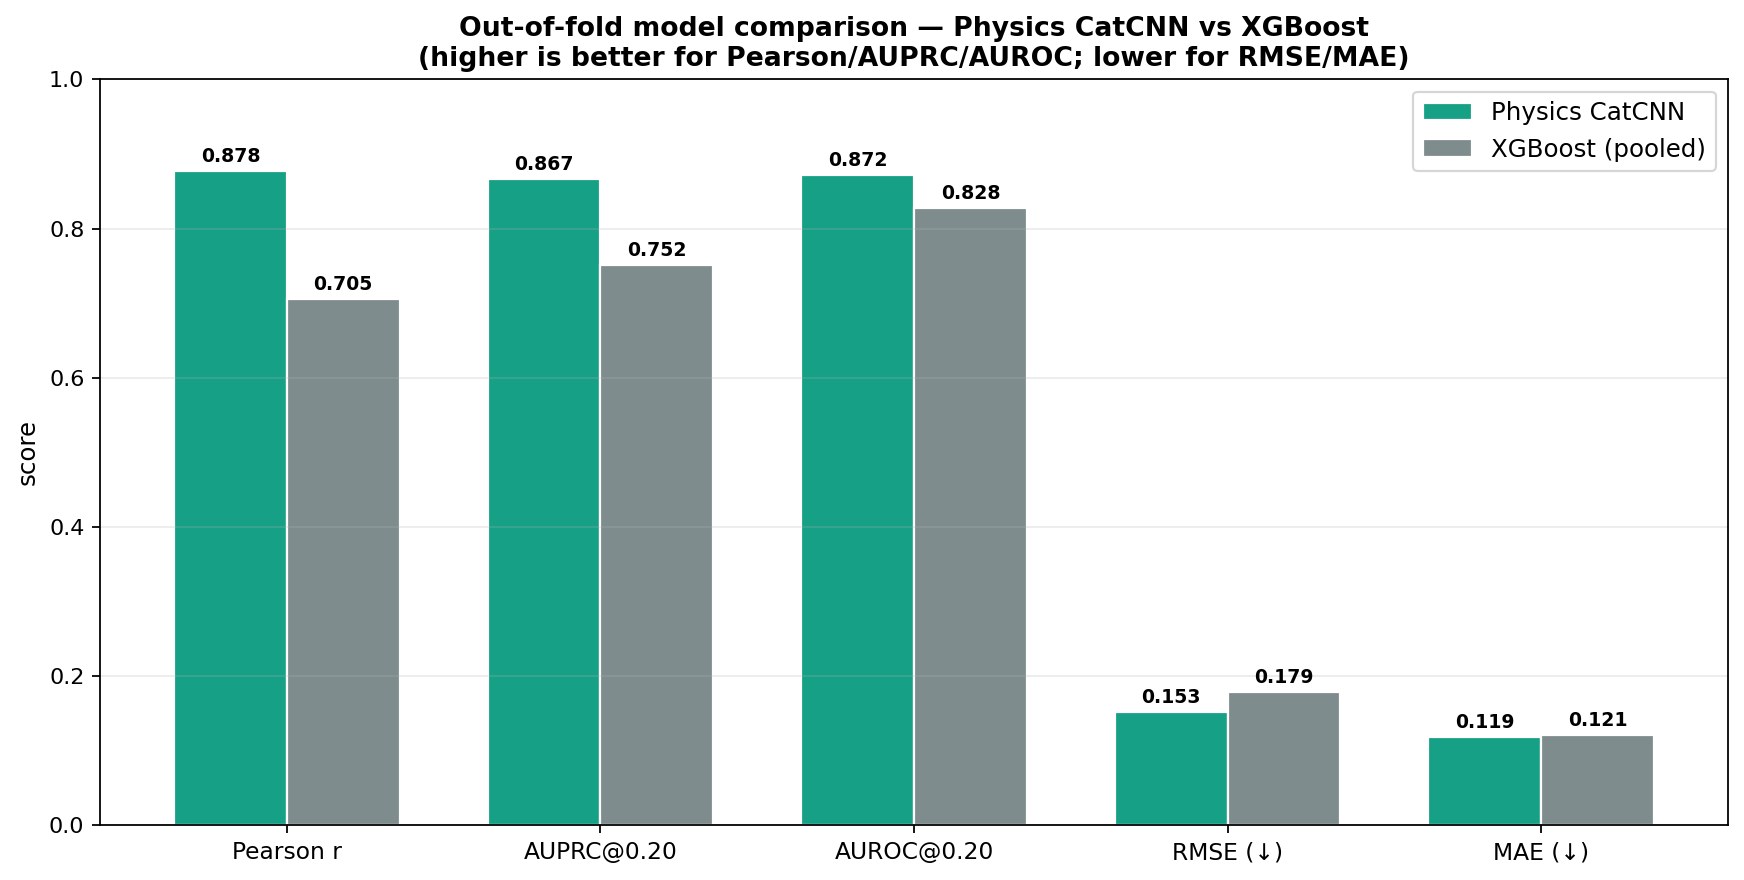
\includegraphics[width=0.92\linewidth]{model_comparison.png}
  \caption{Out-of-fold comparison of the physics-informed CatCNN against
  the XGBoost baseline. The CatCNN is better on every metric: higher
  Pearson, AUPRC, and AUROC, and lower RMSE and MAE---the value of
  treating each event as a spatial field rather than a bag of pooled
  statistics.}
  \label{fig:compare}
\end{figure}

\subsection{What XGBoost reveals about the physics}
\label{sec:eval-importance}
Because XGBoost exposes an interpretable importance ranking, it doubles as
a cross-check that the models key on physically sensible quantities
(Fig.~\ref{fig:xgbimp}). The dominant features are vorticity advection and
frontogenesis at the jet core (VADV and FRONTO at 250\,hPa), deformation
and vorticity just below it (DEF, VORT at 225\,hPa), and the Richardson
number---precisely the frontal and shear diagnostics CAT theory predicts.
The climate indices (ONI, Ni\~no3.4) and cyclic-time features enter only
weakly, quantitatively confirming the exploratory finding
(\S\ref{sec:eda-climate}) that climate is at most a minor modulator and
justifying its placement as identity-initialised FiLM conditioning rather
than a primary input.

\begin{figure}[H]
  \centering
  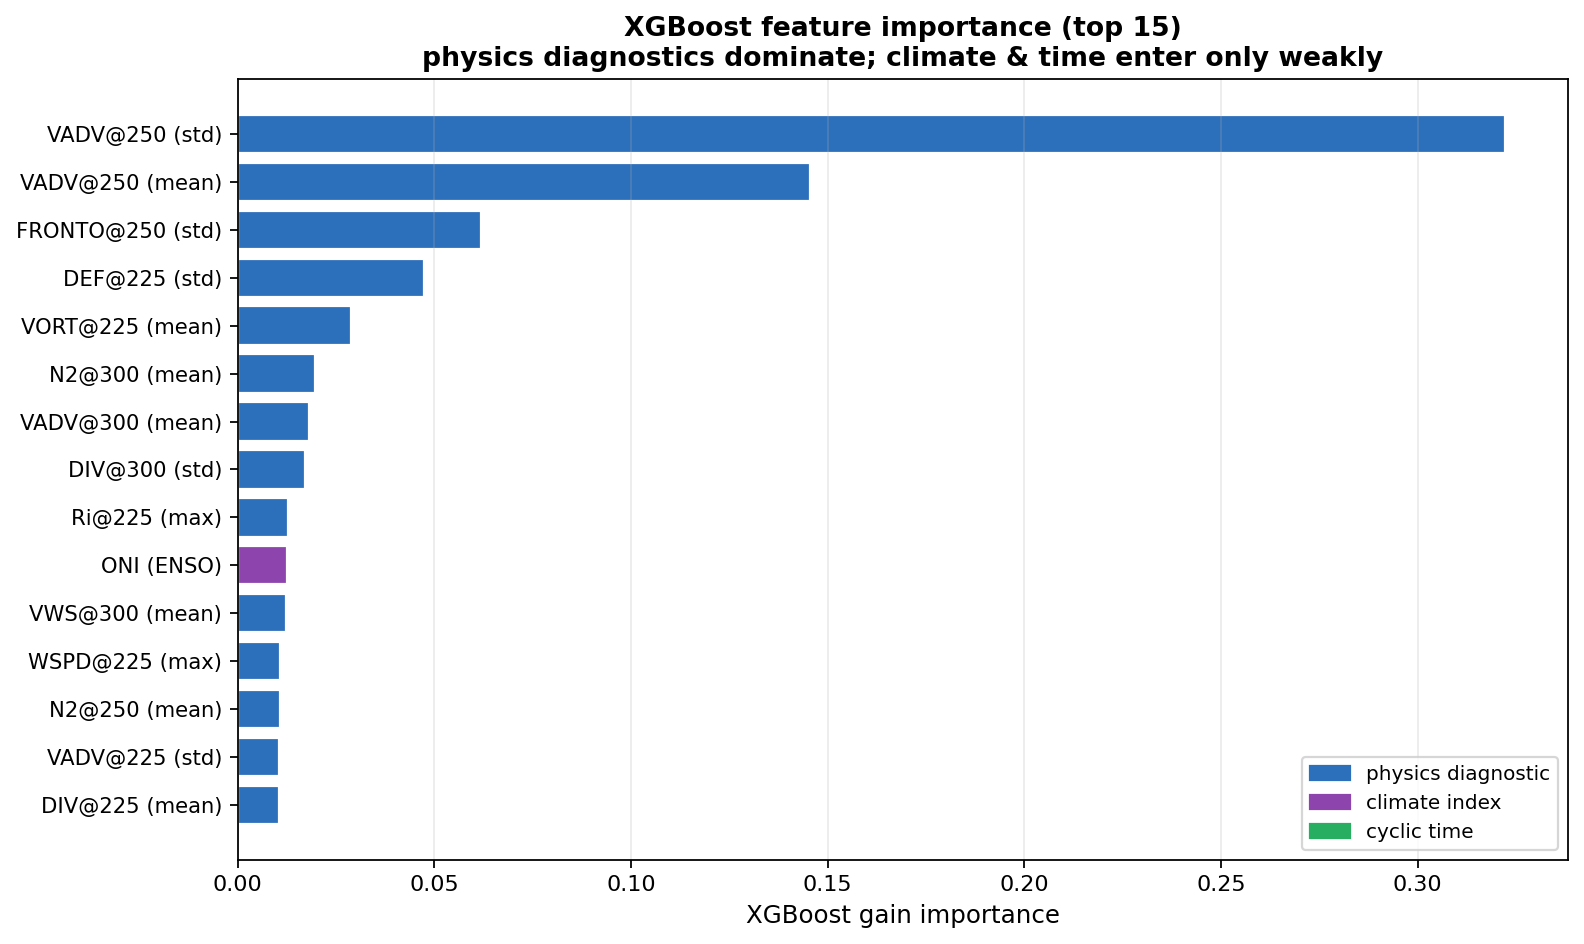
\includegraphics[width=0.82\linewidth]{xgb_importance.png}
  \caption{XGBoost feature importance (top 15). Physics diagnostics---jet-core
  vorticity advection and frontogenesis, sub-jet deformation and
  vorticity, and the Richardson number---dominate; climate indices and
  cyclic time contribute only marginally.}
  \label{fig:xgbimp}
\end{figure}

\subsection{Ablations and remaining figures}
\label{sec:eval-ablation}
Three comparisons remain to complete the evaluation: the satellite-skill
ablation (ERA5-only vs.\ ERA5+satellite on the post-2017 subset, toggling
the stream of \S\ref{sec:arch-sat}) answering \textbf{RQ2}; the GTG
surrogate and Ri-only floor that fill the open rows of
Table~\ref{tab:compare}; and the direct-vs-residual A/B of
\S\ref{sec:residual} with a physics-penalty on/off test. \todo{validation}

% =====================================================================
\section{Discussion}
\label{sec:discussion}
The out-of-fold results tell a coherent story: the dynamical fields carry
strong, generalisable EDR signal (OOF $r=0.878$), and the physics-informed
CNN converts it into skill that clearly exceeds a pooled-feature
gradient-boosting baseline ($r=0.705$) on identical inputs. With only 150
events the binding constraint is \emph{generalisation}, not raw
capacity---and the design meets it by injecting physics as inductive bias
(diagnostic inputs, KH gating, diagnostic-consistency and coherence
penalties) rather than free parameters, which is why a $\sim$80k-parameter
network holds an OOF correlation near $0.88$ where a plain CNN drops to
$0.74$ on held-out data. The remaining quantitative questions---skill
relative to a GTG surrogate and operational benchmarks (ECMWF IFS-CAT),
and the satellite ablation against the coverage caveat of
\S\ref{sec:eda-sat}---await their runs. \todo{validation}

\paragraph{Honest limitations.}
(i)~ERA5's $0.25^\circ$ resolution is coarse relative to the $<$20-mile
CAT patch scale. (ii)~Labels are \emph{scalar only}: the predicted field's
shape is physics-constrained, not label-supervised, until gridded EDR
exists. (iii)~Ground truth is sparse (150 events; satellite on only 64),
and the preliminary overfitting shows how tight that is.
(iv)~Convective-vs-true-CAT ambiguity persists in the post-2017 satellite
subset. (v)~The pre-2017 satellite gap coincides with the most severe
events. (vi)~The decreasing-trend result may carry instrumental
(fleet-drift) signal. (vii)~EMD/EEMD per-IMF variance partitions are
method- and signal-sensitive and are read qualitatively.

% =====================================================================
\section{Conclusion and Future Work}
\label{sec:conclusion}
We have assembled an open, 150-event, multi-source CAT dataset and built a
physics-informed CNN that predicts EDR while respecting CAT physics
through both its inputs (operational diagnostics) and its loss (KH gating,
diagnostic consistency, spatial coherence, climatological bounds), with a
reference CNN, XGBoost, and a GTG-style surrogate as baselines and an
ablatable satellite stream to answer whether imagery adds skill. Under
leakage-safe out-of-fold cross-validation the model reaches Pearson
$r=0.878$ and beats the XGBoost baseline on every metric, settling the
pure-ML half of \textbf{RQ1}: a physics-informed spatial CNN extracts
skill that pooled diagnostic statistics cannot. Closing out RQ1 against a
GTG-style surrogate, and answering \textbf{RQ2} via the satellite
ablation, are the immediate next steps. Future work includes the direct-vs-residual A/B;
promoting the heatmap to dense supervision via sparse-to-dense
ACARS-track labels (changing only the loss); Himawari coverage for global
regions; COSMIC-2 vertical structure; a winter-stratified NAO/AO
teleconnection test; and a real-life test that simulates a weather
phenomenon and predicts CAT hotspots.

% =====================================================================
\bibliographystyle{plainnat}
\bibliography{references}

\appendix
\section{Diagnostic equations (GTG cross-reference)}
The diagnostics of Table~\ref{tab:diag} map to standard GTG equation
labels: Ri (A1), structure-function EDR (A7) and SIGW (A8), frontogenesis
(A9/A10), TI1 (A15), horizontal temperature gradient (A23), wind speed
(A24), $|\mathbf{V}|\cdot$DEF (A28), unbalanced-flow diagnostic (A30),
ABSIA (A34), NCSU1 (A36), Colson--Panofsky (A4), and DTF3 (A6).
\todo{full derivations}

\section{Hyperparameters and search space}
The fixed configuration and search space are: grid~24, levels
225/250/300, depth~3, base width~32, GroupNorm, GELU, max-pool,
dropout~0.1, FiLM hidden~32, satellite MLP~16, head depth~2/width~64,
log-sum-exp $\tau{=}8$; loss $\delta{=}0.1$, $w_{\mathrm{mag}}{=}1$,
$w_{\mathrm{aux}}{=}0.2$, $\lambda_{\mathrm{Ri}}{=}0.1$,
$\lambda_{\mathrm{TI}}{=}0.05$, $\lambda_{\mathrm{TV}}{=}0.01$.
\todo{full table dump}

\end{document}
